\documentclass{article}
\usepackage[utf8]{inputenc}
\usepackage[english]{babel}
\usepackage{graphicx}
\usepackage{amsmath}
\usepackage{amsthm}
\usepackage{xfrac}
\usepackage{float}
\usepackage{amssymb}
\usepackage[font={small}]{caption}
\usepackage{csquotes}
\usepackage{subfig}
\usepackage{booktabs}
\usepackage{tabularx}
\usepackage{titling}
\newcommand{\subtitle}[1]{%
	\posttitle{%
		\par\end{center}
	\begin{center}\large#1\end{center}
	\vskip0.5em}%
}
\usepackage{hyperref}
\captionsetup[figure]{labelfont=bf,textfont={it}}
\captionsetup[table]{position=above,labelfont=bf,textfont={it}}
\graphicspath{{figures/}}



\begin{document}
	
	\maketitle
	
	\section*{Abstract}
	Because of the centrality of data analysis in many human endeavors from science to industry, methods of dealing with faults and errors in data are an important area of study. One such error is the problem of missing data. This thesis provides the reader with a comprehensive introduction to the field of missing data. It describes the concept of missingness mechanisms and how they might impact inference. Imputation is evaluated and found to be a statistically valid technique for addressing missing data in the context of these missingness mechanisms. Various common and intuitive imputation methods such as Complete Case Analysis and Mean Imputation are analysed. Evidence from theory and literature is presented and lead to the conclusion that Multiple Imputation (MI) is the superior method. However, this is contradicted by experimental results, suggesting further study is required to uncover the source of this disagreement. 
	
	\section{Introduction}
	Wherever there is data there tends to be missing data, and missing data can distort or invalidate the conclusions drawn from data. In science and academia data analysis is fundamental to progress, but gathering data in the real world can prove tricky. Take clinical trials of a drug, where dropout can be a serious obstacle to figuring out whether a drug is worth producing or not. Similarly, from tech to traditional heavy industry, data analysis allows for efficiency gains and innovation. However, things from faulty sensors to privacy laws introduce missing data. In this thesis, we shall give an overview of the mathematical theory concerning missing data, as well as some techniques for dealing with the problem. We will first describe common and intuitive solutions, so called \enquote{ad-hoc} solutions, before proceeding to a statistically principled and effective solution: Multiple Imputation (MI). We will approach the problem of missing data from the Bayesian perspective. Other methods motivated from the frequentist perspective, such as likelihood based methods, are available for dealing with missing data, but shall not be explored here. For the sake of brevity and cohesiveness, some topics like congeniality have only been covered in light detail. We refer the reader to Meng [1994], Molenberghs et. al. [2015], and Little and Rubin [2019] for a more in-depth explanation of missing data and non-imputation based techniques.

	
	\section{Terminology and basic missingness theory}
	This section will mostly adhere to the notation of Rubin in \cite{Little2019}, as it is both well established and quite general.
	
	\subsection{What is missingness?}
	When we say an observation is missing, we mean that we have not observed it. The missing observation still has a value, but this value is hidden from us for some reason. The mechanism behind this missingness will be described in detail later in this section. By treating missingness as a probabilistic phenomenon, statistically rigorous tools for dealing with it become available. 
	
	Let the complete data matrix (i.e. with no missing values) $Y=(y_{ij})$ be an $n \times k$ matrix, with the $i^{\text{th}}$ row $y_{i}=(y_{i1}, ..., y_{ik})$ where $y_{ij}$ is the value of variable $Y_{j}$ for observation $i$. Let also the missingness indicator matrix $M = (m_{ij})$ be an $n \times k$ matrix such that $m_{ij} = 1$ if $y_{ij}$ is missing and $m_{ij} = 0$ if $y_{ij}$ is observed. Both $Y$ and $M$ are random variables, and we assume for simplicity that the rows $(y_{i}, m_{i})$ are independent and identically distributed over $i$. It is possible to have more than two possible values for each entry of the $M$, for example when we wish to differentiate between different kinds of non-response. However, we will not explore this in this thesis. Now, given $m_{i}$, we can partition $y_{i}$ into $y^{o}_{i}$ and $y^{m}_{i}$, corresponding to the components that are observed and missing respectively. 
	
	\subsection{The missingness mechanism}
	
	The missingness mechanism is characterized by the conditional distribution of $m_{i}$ given $y_{i}$, i.e. $f_{M|Y}(m_{i}|y_{i}, \theta)$, where $\theta$ denotes unknown parameters. Stated differently, the missingness mechanism characterizes the probability of data being missing given the values observed values of $Y$ and the information that the missing values of $Y$ are missing. 
	
	We distinguish between three different missingness mechanisms by considering how $M$ is related to $Y$ in order of decreasing strictness of assumptions: 
	
	\begin{enumerate}
		\item Missing Completely at Random (MCAR)
		\item Missing at Random (MAR)
		\item Missing Not at Random (MNAR)
	\end{enumerate}
	
	 Rubin [1976] introduced these missingness mechanisms, and they determine which techniques are appropriate to use on a given problem. In practice, they are rarely exactly true, but it will be shown later that assuming them is reasonable in many circumstances.
	
	\subsubsection{Missing Completely At Random}
	 MCAR missingness occurs when, for all and any distinct values $y_{i}$ and $ y^{\ast}_{i}$ in the sample space of $Y$, $$f_{M|Y}(m_{i}|y_{i}, \theta) = f_{M|Y}(m_{i}|y^{\ast}_{i}, \phi), \quad \exists \theta, \phi$$ where $\theta$ and $\phi$ denote unknown parameters. In other words, the probability of missingness is independent of both the observed and the missing data. This means that we can view the observed data as a random sample of the complete data.
	
	\subsubsection{Missing At Random}
	In this case, for all i and any distinct values $y^{m}_{i}, y^{m\ast}_{i}$ in the sample space of $Y^{m}_{i}$, we have that the following equation holds: $$f_{M|Y}(m_{i}|y^{o}_{i}, y^{m}_{i}, \theta) = f_{M|Y}(m_{i}|y^{o}_{i}, y^{m\ast}_{i}, \phi), \qquad \exists \theta, \phi$$
	This means that the probability of missingness, conditioned on the observed data, is independent of the missing data. Assuming MAR is less restrictive than MCAR, and may be considered a more plausible assumption in a real world situation. 
	
	\subsubsection{Missing Not At Random}
	If the above equation does not hold for some $i$ and some $y^{m}_{i}, y^{m\ast}_{i}$, then the missingness mechanism is called missing not at random (MNAR). In this situation, the probability of missingness is dependent on the missing data even after conditioning on the observed data. Put differently, this means that the underlying values of the missing data influence the probability of data being missing. Thus the the missingness mechanism cannot be characterised from the available data in the way that MAR can.
	
	\subsection{Illustrative example}
	
	The following example illustrates the three different types of missingness.
	
	Suppose you are doing a study in which you want to investigate people's sleep patterns. You send $N$ people a survey asking them for the average amount of sleep they got each night in 2018. A year later, you decide to send a follow-up survey for 2019. We consider 2018 and 2019 to be stochastic variables. Table 1 shows a simulation of such a study.
	
	\begin{table}[]
		\begin{tabular}{ccccc}
			\multicolumn{1}{l}{2018} & \multicolumn{1}{l}{2019 (Complete)} & \multicolumn{1}{l}{2019 (MCAR)} & \multicolumn{1}{l}{2019 (MAR)} & \multicolumn{1}{l}{2019 (MNAR)} \\ \hline
			8.9                      & 7.4                                 & 7.4                             & 7.4                            & NA                              \\
			9.4                      & 7.3                                 & 7.3                             & 7.3                            & NA                              \\
			8.4                      & 7.9                                 & NA                              & 7.9                            & NA                              \\
			5.3                      & 6                                   & NA                              & NA                             & NA                              \\
			11.1                     & 7.4                                 & 7.4                             & 7.4                            & NA                              \\
			8.4                      & 10.7                                & NA                              & 10.7                           & 10.7                            \\
			6.4                      & 8.8                                 & NA                              & NA                             & 8.8                             \\
			5.6                      & 3.5                                 & NA                              & NA                             & NA                              \\
			5.6                      & 7.1                                 & 7.1                             & NA                             & NA                              \\
			8.2                      & 6.9                                 & 6.9                             & 6.9                            & NA                              \\
			6.6                      & 5.4                                 & NA                              & NA                             & NA                              \\
			6.6                      & 6.7                                 & NA                              & NA                             & NA                              \\
			8.6                      & 9.2                                 & NA                              & 9.2                            & 9.2                             \\
			7.7                      & 6.1                                 & 6.1                             & NA                             & NA                              \\
			11.2                     & 8                                   & NA                              & 8                              & 8                              
		\end{tabular}
	\caption{\label{tab:tab1}Simulated data for $N = 15$ individuals drawn from a bivariate normal distribution with $\mu_{2018} = \mu_{2019} = 7.5$, $\sigma_{2018} = \sigma_{2019} = 2$, and a correlation $\rho = 0.3$. The first two columns show the complete data for 2018 and 2019, while the other three columns show the values for 2019 after imposing missingness by the three methods discussed earlier.}
	\end{table}

	In the MCAR scenario, we see a random spread of missing data, i.e. a random subset of those who answered the 2018 survey also answered the 2019 one. Now, suppose that the amount of sleep people got in 2018 affected how likely they were to answer the 2019 survey. Those who slept little in 2018 were less likely to answer in 2019, and conversely with those who slept more. This is MAR, since the missingness of the 2019 entries depends on the values for 2018. For the final column, suppose our earlier conjecture is instead true for 2019: those who slept little in 2019 were less likely to answer the survey in that year. This is an example of MNAR, since the missingness of the 2019 entries depends on the values for those entries. Remember, the full dataset exists, but it has been hidden from us due to some mechanism.
	
	
	\subsection{The validity of missingness mechanisms}
	
	In most real world scenarios, we only have the data at hand to inform us about the missingness mechanism. Unfortunately, we cannot infer the missingness mechanism from data \cite[P.9]{Molenberghs2015}. We can check the validity of MCAR against MAR, but only under the unverifiable assumption that the data is not MNAR \cite[P.8]{Molenberghs2015}. Neither can we use the data at hand to support or refute one specific MNAR mechanism over another \cite[P.10]{Molenberghs2015}. Finally, MAR cannot be checked empirically against MNAR. We therefore have to assume the missingness mechanism in practice. Most often it is beneficial to assume MAR, as it tends to yield good empirical results even when the assumption does not completely hold. 
	
	\section{Imputation}
	
	\subsection{What is imputation?}
	Imputation refers to the substituting, or \enquote{filling in}, of missing values with plausible estimates. Often there much information available in the data at hand, and utilising this can lead to better performance. The main strength of imputation is that it does not require us to change our desired analysis technique.  In certain situations, a researcher might have more data than they intend to include in their analysis model. This extra data can be used in the imputation process to produce a better imputation, but can introduce bias or variance in parameter estimates. The concept of congeniality, which we will define shortly, helps us overcome some of these difficulties. Another very practical benefit, and a strong argument for the use of imputation, is the performance gains to be had from using it. Examples can be seen in \cite{madley-dowd_proportion_2019}, \cite{Schafer2002}, and \cite{Sterne2009}, as well as in the experiments section.
	
	The model based approaches of this thesis use both the Bayesian and frequentist paradigms in complementary ways. The Bayesian approach is used to create the imputation procedure, while the frequentist one evaluates their results. The Bayesian paradigm allows us to effectively model the unknown given the known, and makes assumptions explicit, both highly desirable when imputing missing data. The frequentist paradigm is the one which is by far most common when doing inference, so it is natural that it is under that paradigm we evaluate performance.
	
	\subsection{What is valid inference?}
	An essential question when using imputation is if, and how, it might distort inference. However, to answer this question we need to have an idea of what valid inference is. A valid inference, according to Rubin \cite{rubin_multiple_1996}, is one in which nominal significance levels (denoted by $\alpha$ and often set at $\alpha = 0.05$) describe characteristics of a distribution for confidence interval estimation and hypothesis testing. This can be further refined into \enquote{randomization validity} and \enquote{confidence validity}. The former Rubin describes as \enquote{actual interval coverage = nominal interval coverage}, for interval estimates, and  \enquote{actual rejection rate = nominal rejection rate}, for hypothesis tests. Randomization validity is of course desirable, but not always achievable, and so Rubin introduces confidence validity as a looser criterion. It is defined as \enquote{actual interval coverage $\geq$ nominal interval coverage}, for interval estimates, and \enquote{actual rejection rate $\geq$ nominal rejection rate}, for hypothesis testing. It is this last version of inferential validity that we shall be referring to whenever we talk about valid inference. It has been shown \cite{Xie2017}, \cite{Meng1994}, \cite{rubin_multiple_1996} that Bayesian models like the Multiple Imputation (MI), which we will describe in detail in a later section, yield valid inference.
	
	\subsection{Congeniality: when the imputation and analysis models differ}
	Congeniality is an important concept in imputation and has a big impact on the statistical validity of imputation. In short, when the analysis model differs substantially from the imputation model we say that they are uncongenial. Such differences might cause the subsequent analysis to be biased, or in the worst case, invalid. There are many reasons for such difference, for example, one might wish to include as many variables as possible in the imputation model to achieve an accurate imputation, while at the same time only being interested in only a subset of the covariates and the relationship between these. We will not go into detail about what specifically constitutes a \enquote{substantial difference}, and refer to \cite{Meng1994} for a detailed description and explanation. However, an important finding by Meng is that even with an uncongenial imputation model, MI still outperforms methods that ignore missing data. This will be borne out in the experiments section.
	
	
	\section{Techniques of interest}
	To properly evaluate the performance of MI, we should compare it to other similar and commonly used techniques, i.e. techniques that manipulate the dataset by either imputing or removing values. When choosing to apply a method it is important to keep two questions in mind. First, does the method under consideration give us consistent estimators for our model? Second, does the method give us appropriate measures of precision? How the following methods answer these questions will determine which methods are preferable. For a more in-depth description and examples of these methods we refer the reader to \cite{Molenberghs2015}.
	
	There is another competing set of methods which we should touch on briefly before continuing: likelihood-based methods. These methods focus on maximising the likelihood function directly. Under MAR, the missing data can be ignored in calculations, leading to a much more tractable problem. However, given congeniality, more advanced imputation methods like multiple imputation tend to outperform likelihood-based methods for small sample sizes, while delivering similar performance for large sample sizes \cite{schafer_multiple_2016}.
	
	\subsection{Ad hoc methods}
	This section is mostly adapted from Chapter 2 of \cite{Molenberghs2015} Although ad hoc is pejorative in certain circumstances, it is used here to indicate that the methods below are motivated by convenience rather than any methodological concern.
	
	\subsubsection{Case deletion, also called Complete Case Analysis}
	Probably the most common technique in use for dealing with missing data, Complete Case Analysis (CCA) involves restricting analysis to entries with complete data. For those familiar with programming, a typical example would be to remove all rows from a dataframe with NaN entries. The first and most obvious problem with this approach is that it drastically reduces the amount of useable data. CCA holds an intuitive appeal, as it is both exceedingly simple to implement, and with the only seeming downside being a loss in accuracy. However, depending on the missingness mechanism, CCA can actually introduce bias into an analysis. For example, suppose you want to find the mean and standard deviation in the height of a population. If for some reason you lack all entries for people above 200cm, then disregarding these missing entries in a CCA will lead to biased estimates for both the mean and variance. An implicit assumption, therefore, of CCA is that the observed data is a random sample of the underlying distribution. This means that CCA implicitly assumes MCAR, and we see in \cite{Schafer2002} that we get unbiased inference in this scenario, though with lower accuracy depending on the amount of missing data. However, as with the height example, deviation from MCAR can introduce bias. See \cite{Schafer2002} for examples of how inference is affected.
	
	\subsubsection{Mean imputation}
	Another common practice involves substituting the missing values with the mean of the observed values for that variable. As stated in Schafer and Graham \cite{Schafer2002}, this has the effect of preserving the mean of the distribution one wishes to draw inference about, but distorts other parameters such as variance and covariance. Covariance especially is distorted due to mean imputation taking only the variable under consideration as input. In addition to this, the technique breaks down when confronted with categorical variables for which a mean has a less obvious meaning, and it is clear how a majority vote imputation might skew the data.
	
	
	\subsubsection{Last Observation Carried Forward}
	Last Observation Carried Forward (LOCF) is mostly used in longitudinal studies where individuals drop out, withdraw, or are lost over the course of the studies. LOCF involves imputing the missing values for an individual with the last observed value for that individual. By replicating already existing values, LOCF has a dampening impact on the variance estimate. Additionally, LOCF produces biased estimators in all except very specific MNAR circumstances \cite{KenwardM.G.andMolenberghs2009}. With LOCF, we are effectively assuming that for each individual that drops out, their responses do not change at all for the remainder of the study, a highly unrealistic assumption. It can be concluded, therefore, that LOCF is the worst imputation method of those mentioned here, and all the other methods are preferable. We round off by quoting \cite[P. 40]{Molenberghs2015} that\enquote{LOCV is neither valid under general assumptions nor based on statistical principles, it is not a sensible method, and should not be used}.
	
	\subsubsection{Regression}
	Regression imputation functions by regressing the variable(s) with missing entries on the fully observed variables, or subsets that are fully observed. To illustrate this, let us consider the simplest case, with one fully observed variable $X$ linearly related to a variable $y
	Y$ with missing data. Fitting a regression of $X$ on $Y$, we have$$Y_{i} = \beta_{0} + \beta_{1}x_{i} + \epsilon, \qquad \epsilon \sim N(0,1) \qquad i\in(0,...,n)$$ Obtaining estimates of the regression parameters $\hat{\beta_{0}}$ and $\hat{\beta_{1}}$ allows us to impute $E(y_{i}) = \hat{\beta_{0}} + \hat{\beta_{1}}x_{i}$. A variation on this method is to use the regression to specify the parameters of a normal distribution $Y ~ N(X\beta, \sigma_{y})$ from which to draw our imputation values.  This is the best of the ad hoc methods, as it gives us much more plausible imputations that vary more like the true data \cite[P. 37]{Molenberghs2015}. However, even in this simple case it yields imputations that tend to be less variable than the observed data. Therefore, using these imputations in inference will most often lead to underestimating standard errors and p-values. If there are non-linear relationships in the data, this method's performance breaks down.
	
	\section{Statistically principled imputation}
	The methods in this section are motivated from a desire to preserves the distributional qualities in the data. For inference, this would be parameter values of a distribution and their variance and covariance. 
	
	
	\subsection{Single imputation using conditional distributions}
	Single imputation is the building block of MI, and many of its deficiencies are corrected for when expanded to MI. It can be done in a variety of ways, but the most straightforward and easy to understand is the following: create a joint posterior distribution of your missing data given your observed data, i.e. $f(Y^{m}|Y^{o}, M)$. Draw from this distribution to fill in your dataset, then perform your desired analysis. How you specify the missing data model can determine the efficacy of this method, but it is otherwise uncomplicated. We will therefore focus the majority of our analysis on the MI case.
	
	\subsection{Multiple imputation}
	One sizeable weakness of the earlier imputation methods is that they use points as estimates of distributions. Hence, subsequent measures of precision are biased downwards. Multiple imputation solves this problem by creating multiple imputed datasets drawn from $f(Y^{m}|Y^{o}, M)$, running the desired analysis procedure on each, and then combining the results. This preserves the distributional variation in the missing data, and leads to better variance estimates. It can be quite computationally expensive, especially for large data sets, but recent increases in available computation power has made this concern less of an issue. Many previous objections to MI regarding inference concerned MI using a low number of imputed datasets $M$, typically between 5 and 10 \cite{Meng1994}. With larger $M$ and careful combining of the resulting analyses, one can achieve strong results in a large number of situations, see \cite{Xie2017}), \cite{Meng1994}, \cite{rubin_multiple_1996}, and \cite{madley-dowd_proportion_2019}.
	
	Multiple imputation can be thought of as three distinct steps:
	\begin{enumerate}
		\item $M$ imputed datasets are generated through repeated random draws from the predictive distribution of the missing values, $f(Y^{m}|Y^{o}, M)$, under a particular model for missingness.
		\item The intended analysis is performed separately on all $M$ datasets
		\item The results of the analyses are combined using Rubin's or Meng's rules (which we will describe shortly) to create a single MI result.
	\end{enumerate}
	It should be noted that even though there is no strict mathematical proof that MI yields valid inference in the case of finite $M$, the empirical evidence in the literature so far referenced presents a strong case that MI is a useful tool. Comparing it to the other methods available, one finds that alternatives are on the whole less effective.
	
	\subsubsection{Specifying the imputation model}
	
	To create an accurate model for the missing data, we often want to include as many covariates as possible. Madley-Dowd et al. [2019] have shown that even mildly correlated auxiliary variables can improve subsequent inference. By auxiliary, variables we mean variables not included in the analysis model. For example, imagine we have data on 1000 people's age, height, and weight. Suppose we wish to find the relationship between age and weight, but we are missing some of the weight data. Since height is correlated with weight, i.e. it contains some information about the distribution of weight, it makes sense to include it in our imputation model, despite not using it in our analysis. This leads us to make repeated random draws from $f(Y^{m}|Y^{o}, M, A)$, where $A$ represents auxiliary variables. Whether or not to include auxialiary variables can be either a cause and a cure for uncongeniality depending on the situation. Meng [1994] cautions against the use of less general imputation models (e.g. ignoring covariates/auxiliary variables).
	
	\subsubsection{Rubin's rules}
	
	At step 2 of MI, we have $M$ sets of parameter estimates and their variances: $\hat{\theta}_{i},\hat{Var_{i}}, \quad i=0,...,M$. The next step is to combine these into a single estimate. Under congeniality, Rubin's combining rules suffice for giving us statistically valid estimates \cite{Meng1994}. The parameter estimate is simply the average $$\bar{\theta} = \frac{1}{M}\sum_{i=0}^{M}\hat{\theta}_{i}$$ and the variance associated with $\bar{\theta}$ is given by 
	 
	\begin{equation}
		T = \overline{Var}+(1+\frac{1}{M}B)\tag{*}
	\end{equation}
	
	where $$\overline{Var} = \frac{1}{M}\sum_{i=0}^{M}\hat{Var}_{i}$$ measures the within imputation variability and $$B = \frac{1}{M-1}\sum_{i=0}^{M}(\hat{\theta_{i}}-\bar{\theta})(\hat{\theta_{i}}-\bar{\theta})^{T}$$ measures the between imputation variability. The adjustment $(1+\frac{1}{M}B)$ in equation $(*)$ is due to the finite number of imputations. If we let $M\rightarrow\infty$ then we achieve asymptotic equality to the true variance estimate.
	
	Xia and Meng [2017] state that \enquote{When the imputation model class and the (embedded) analyst’s model class
		differ, the behavior of Rubin’s rules becomes very complicated, capable of producing inconsistent variance estimators, a matter that has received recurrent
		criticisms}. They argue that in the uncongenial case, which is often the rule rather than the exception, doubling Rubin's variance measure will never underestimate the true variance. This holds for any degree of uncongeniality, and provides a surprisingly simple solution to the problem of uncongeniality. For univariate data, Xia and Meng  [2017] suggest replacing $T$ with $\tilde{T}= (\sqrt{\overline{Var}}+\sqrt{B})^{2}+\frac{1}{M}B$. These methods may be viewed as highly conservative, but in the context of MI where uncongeniality between analysts and imputer is unknown and potentially large, it pays to be as insured as possible against invalid inference. However, even if these methods are not used and the models are uncongenial, we note that Meng [1994] has shown that MI is still superior to CCA.
	
	\subsubsection{Potential pitfalls and criticism}
	The following arguments apply for imputation in general, but we will consider them in the context of MI. When there is missing data in several variables of different types, for example continuous and binary, and there exists hierarchical structure in the data, specifying the imputation model can be quite difficult. A solution to the problem is using chained equations, where one has a univariate model for each variable with missing data and iteratively draws from this. Despite good empirical results, this method lacks the theoretical justification of drawing from a fully specified conditional distribution \cite{Little2019}, and so is at best a partial solution. Another danger is that improper specification of the imputation model can cause uncongeniality and so one needs to exercise care when using MI. Finally, imputation procedures based on drawing from conditional distributions tend to assume that these distributions are normal. In certain cases this requires us to transform the data.
	
	Taking all this into account, it is important to see MI in the context of the options available to someone working with data. As we have established earlier, simply ignoring missing data can lead  to serious biases, while alternative methods tend to negatively effect estimates and/or their variance. Since there is no option to \enquote{do nothing}, MI presents itself as a useful way of dealing with missing data.
	
	\section{Experiments}
	
	
	\subsection{MICE}
	We have chosen to use the MICE package for R \cite{Buuren2011} for our experiments. There are two main reasons for this. One is the performance: MICE is able to deal with the complex scenario of mixed variable types as described earlier. MICE functions by drawing from univariate conditional distributions for all the variables with missing data, i.e for a variable $Y_{i}$ we draw from the predictive distribution $p(y_{i}|y_{0}, ... y_{j}), \quad i\neq j$ for each i in an iterative process. This solves the problem of complex data mentioned earlier, and despite the lack of theoretical justification, its performance is comparable to the fully specified conditional distribution approach \cite{Lee}, \cite{Little2019}.
	
	\subsection{Synthetic example}
	
	In this section we will provide a simple experiment to explore the efficacy of MI. We will look at a simple linear regression with a single covariate defined by the model $Y_{i} = \beta_{0} + \beta_{1}x_{i} + \epsilon, \qquad \epsilon \sim N(0,1) \qquad i\in(0,...,n)$. Missingness will be simulated in both $X$ and $Y$. Data was generated by drawing from a bivariate normal distribution $$[Y X] \sim N(\begin{bmatrix}
	0 \\
	0 \\
	\end{bmatrix},\begin{bmatrix}
	1 & 0.8 \\
	0.8 & 1 \\
	\end{bmatrix})$$ The true regression coefficient is then $\beta_{1} = 0.8$. In our experiment we draw 1000 data points from this distribution. MCAR was simulated by removing the first p values in the data set. MAR was simulated using the logit function where the probability of an observation being missing was equal to $\frac{1}{1+e^{-(Y + \alpha)}}$ when simulating missingness in X, and $\frac{1}{1+e^{-(X + \alpha)}}$ when simulating missingness in $Y$. $\alpha$ was chosen such that we achieved the desired percentage of missing data. MNAR was simulated using the same logit function, but in this case the probability of $Y$ missing was dependent on $Y$. The number of imputations $M$ was set to 20. We will look at the following metrics to evaluate the performance of MI:
	
	\begin{enumerate}
		\item Size of the confidence interval of $\beta_{1}$
		\item Coverage of the confidence interval
		\item Bias
	\end{enumerate}
	
	We will compare the performance of MI to an equivalent analysis performed with CCA for reference. Our experiment was then conducted in the following manner:
	
	\begin{enumerate}
		\item Draw 1000 observations from the distributions of $[Y X]$
		\item Simulate 5, 10, 20, 40, 60, 80, and 90 percent missingness under different missingness mechanisms.
		\item Create linear models for each of these 7 datasets based on CCA and MI
		\item Repeat 1000 times
		\item Evaluate the results based on the above metrics.
	\end{enumerate}

	
	\subsubsection{MCAR}
	
	\begin{figure}[H]
		\centering
		\subfloat[$\beta_{1}$ estimate with CCA]{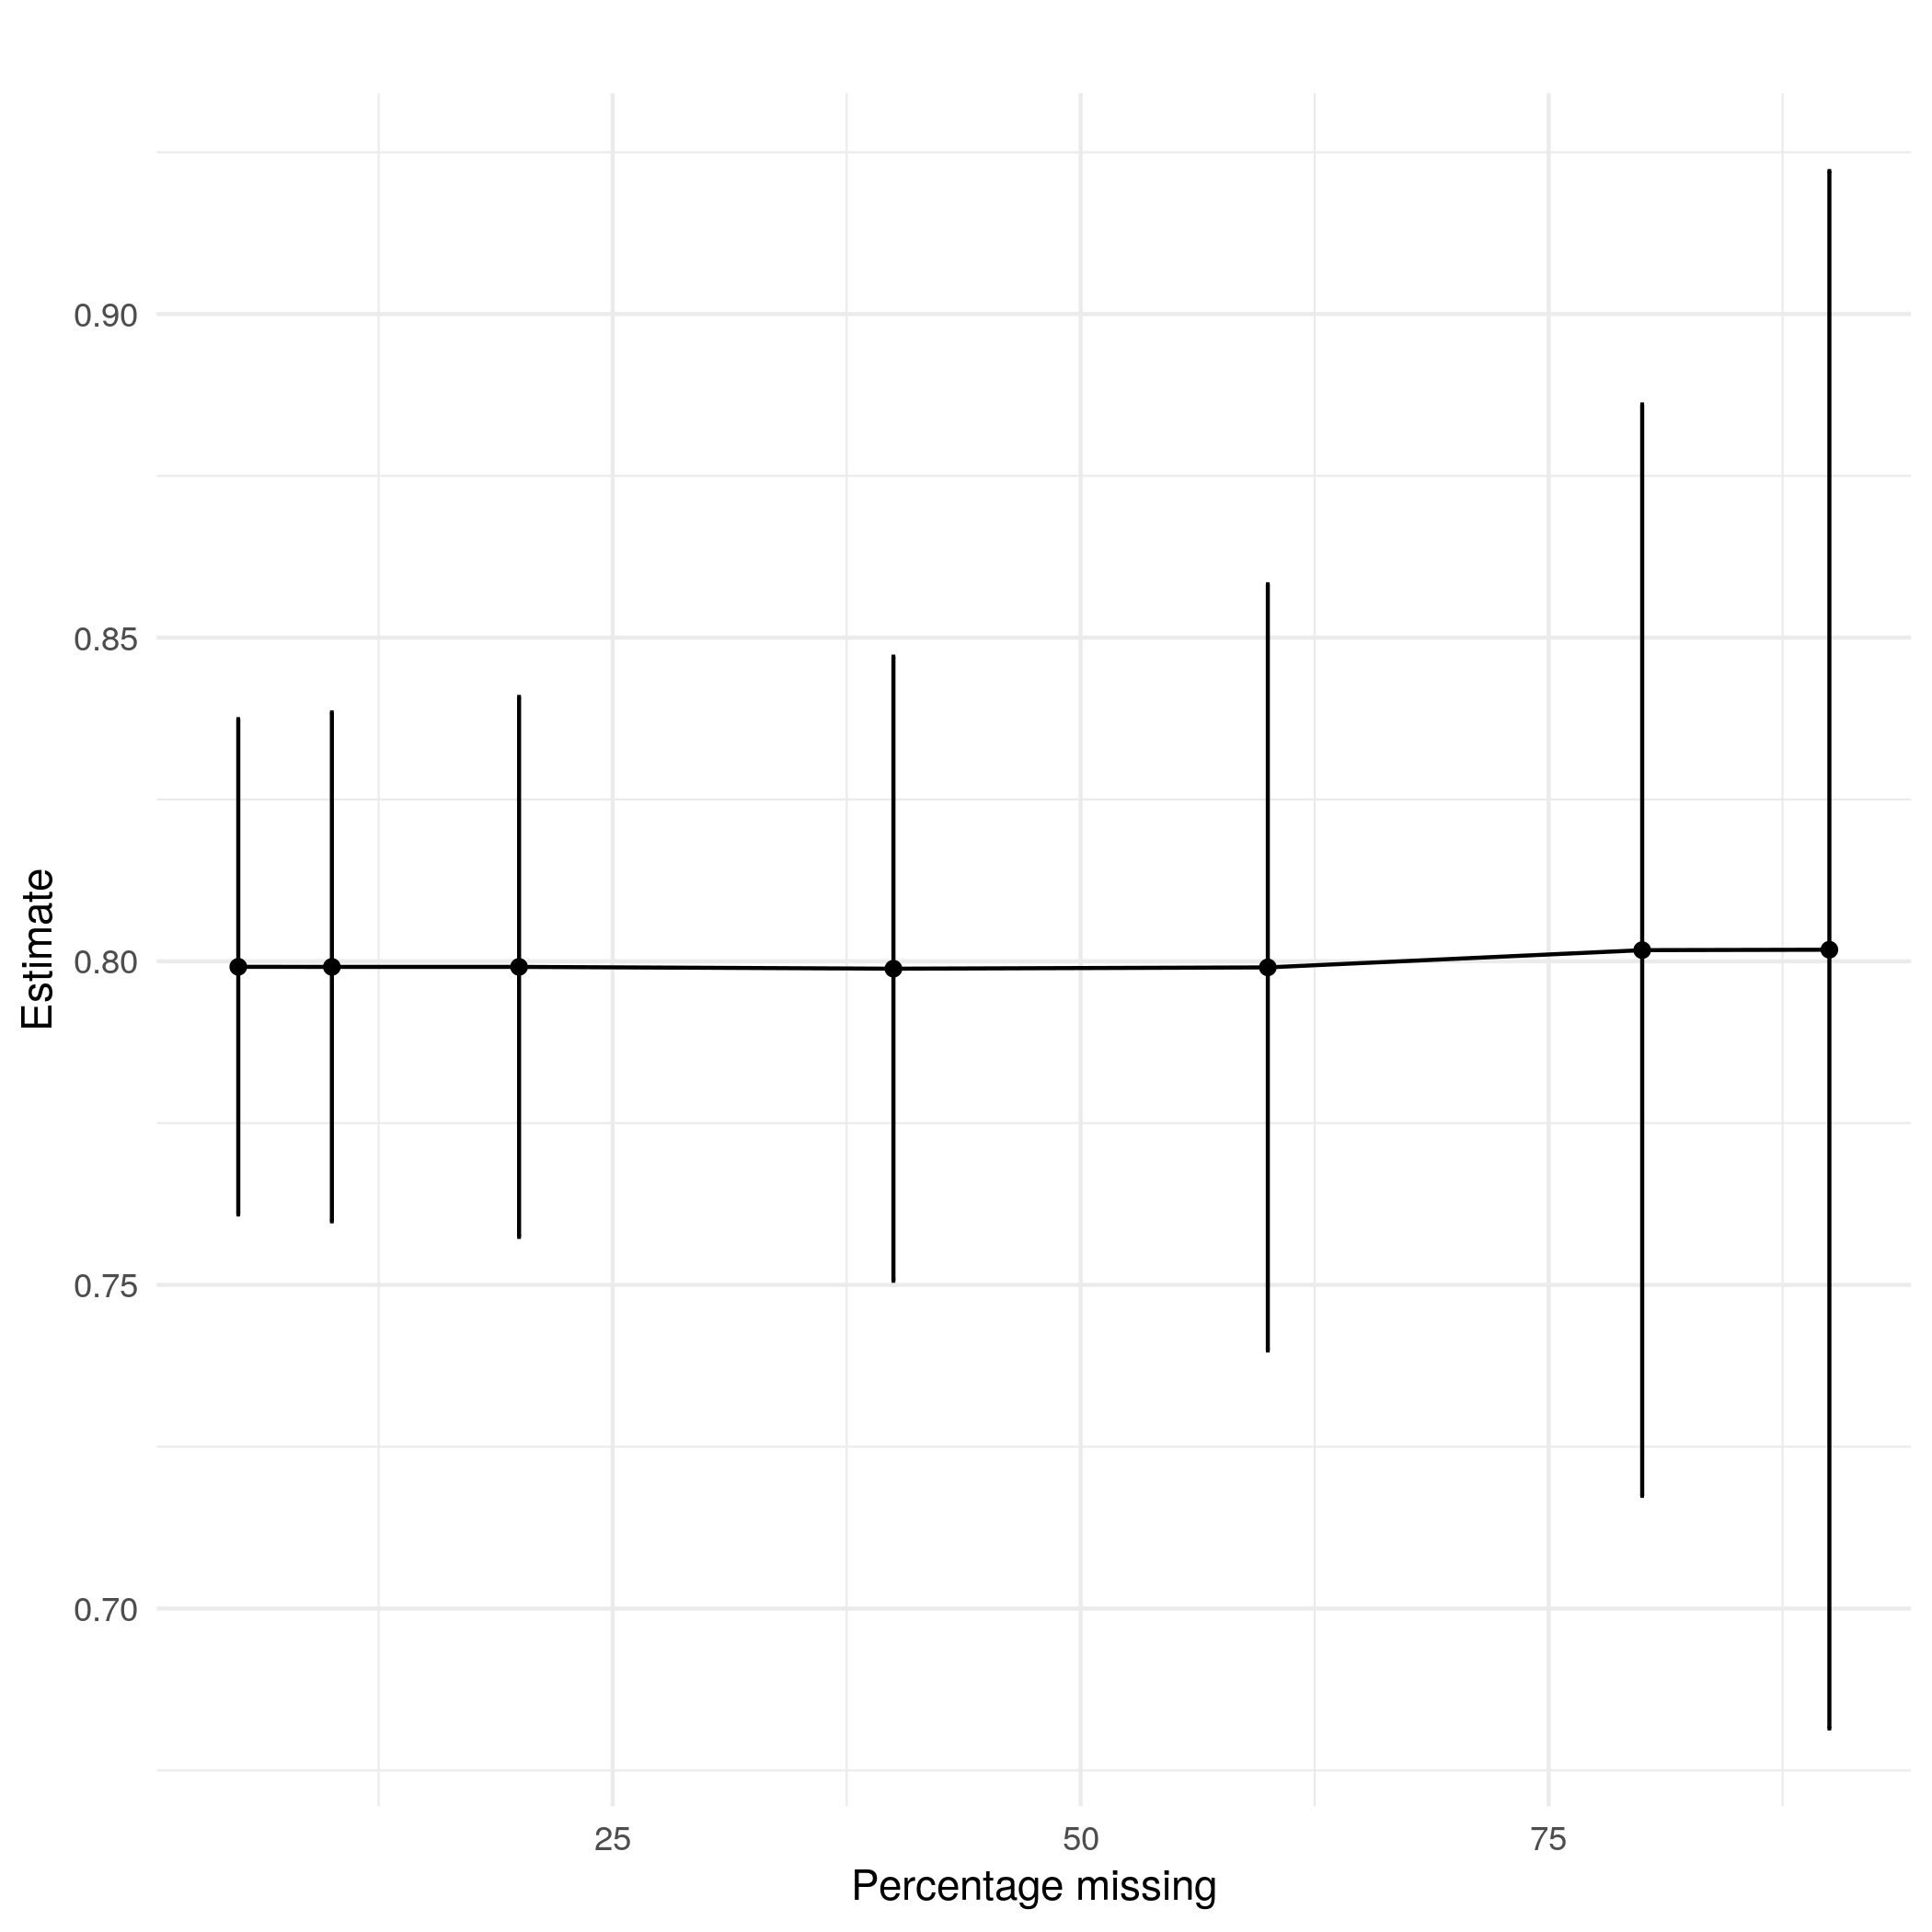
\includegraphics[width=0.4\textwidth]{mcar_estimate_cca.png}}
		\quad
		\subfloat[$\beta_{1}$ estimate with MI]{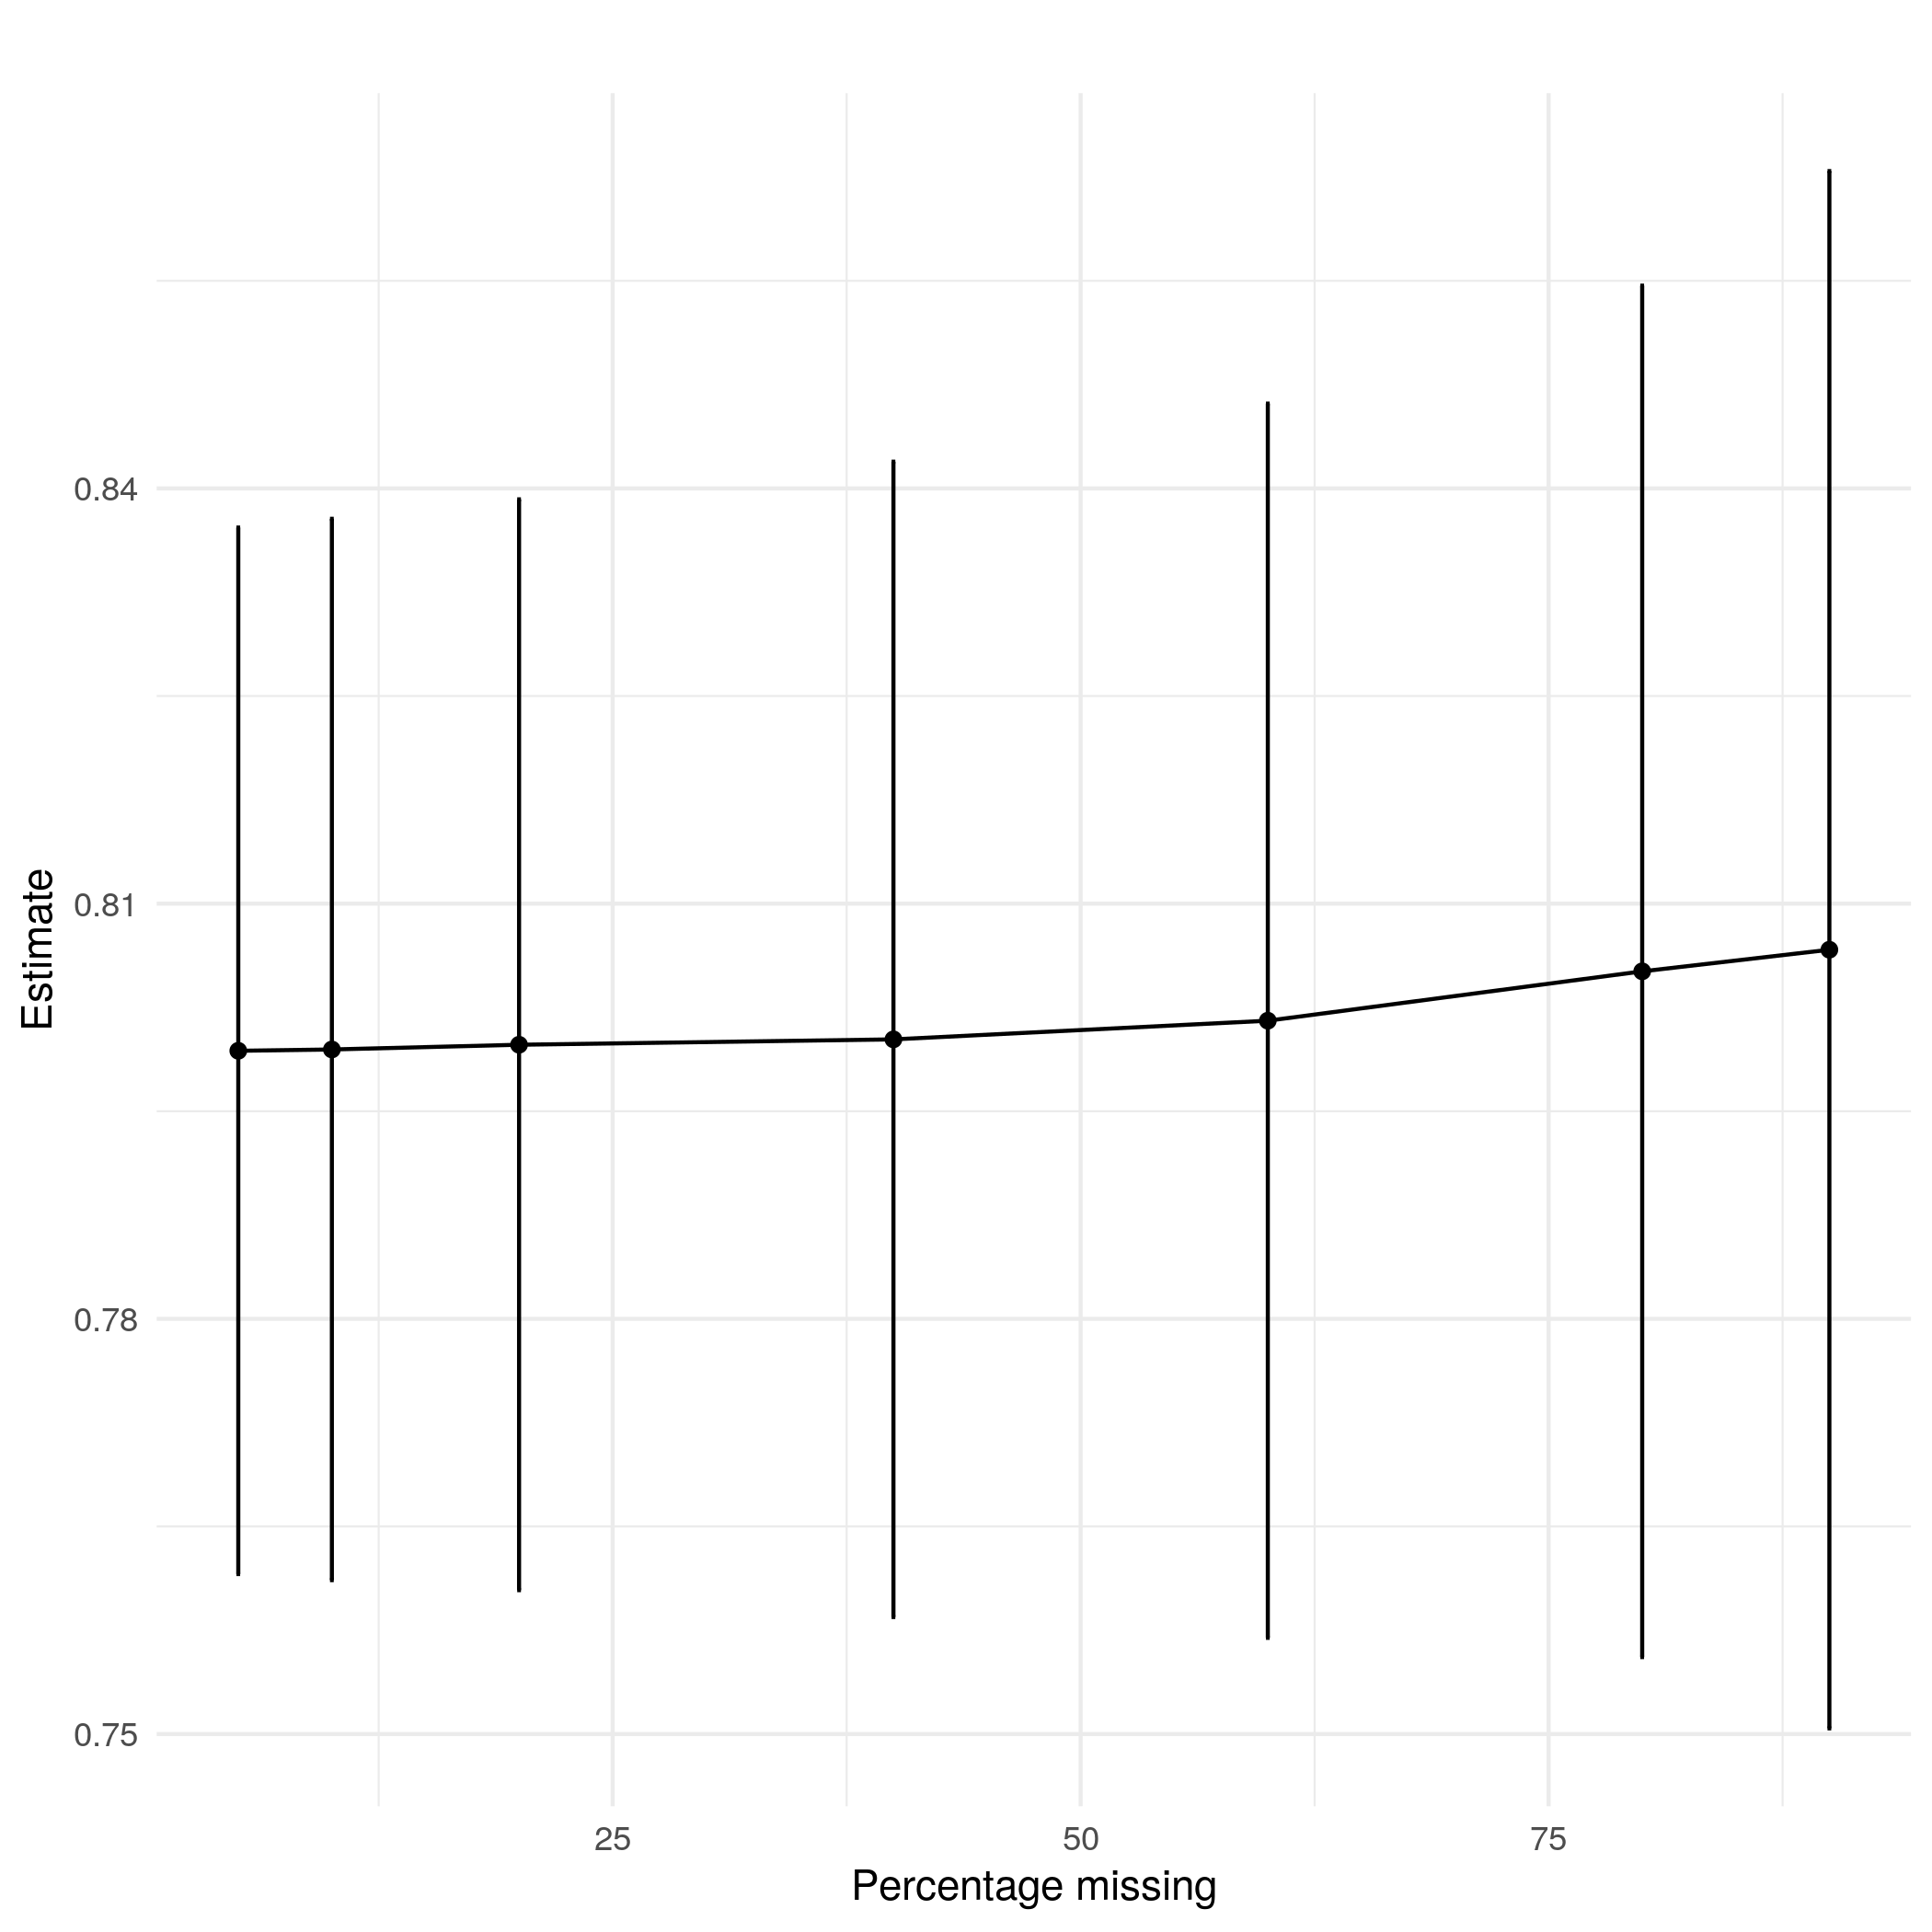
\includegraphics[width=0.4\textwidth]{mcar_estimate_mi.png}}
		\\
		\subfloat[Coverage]{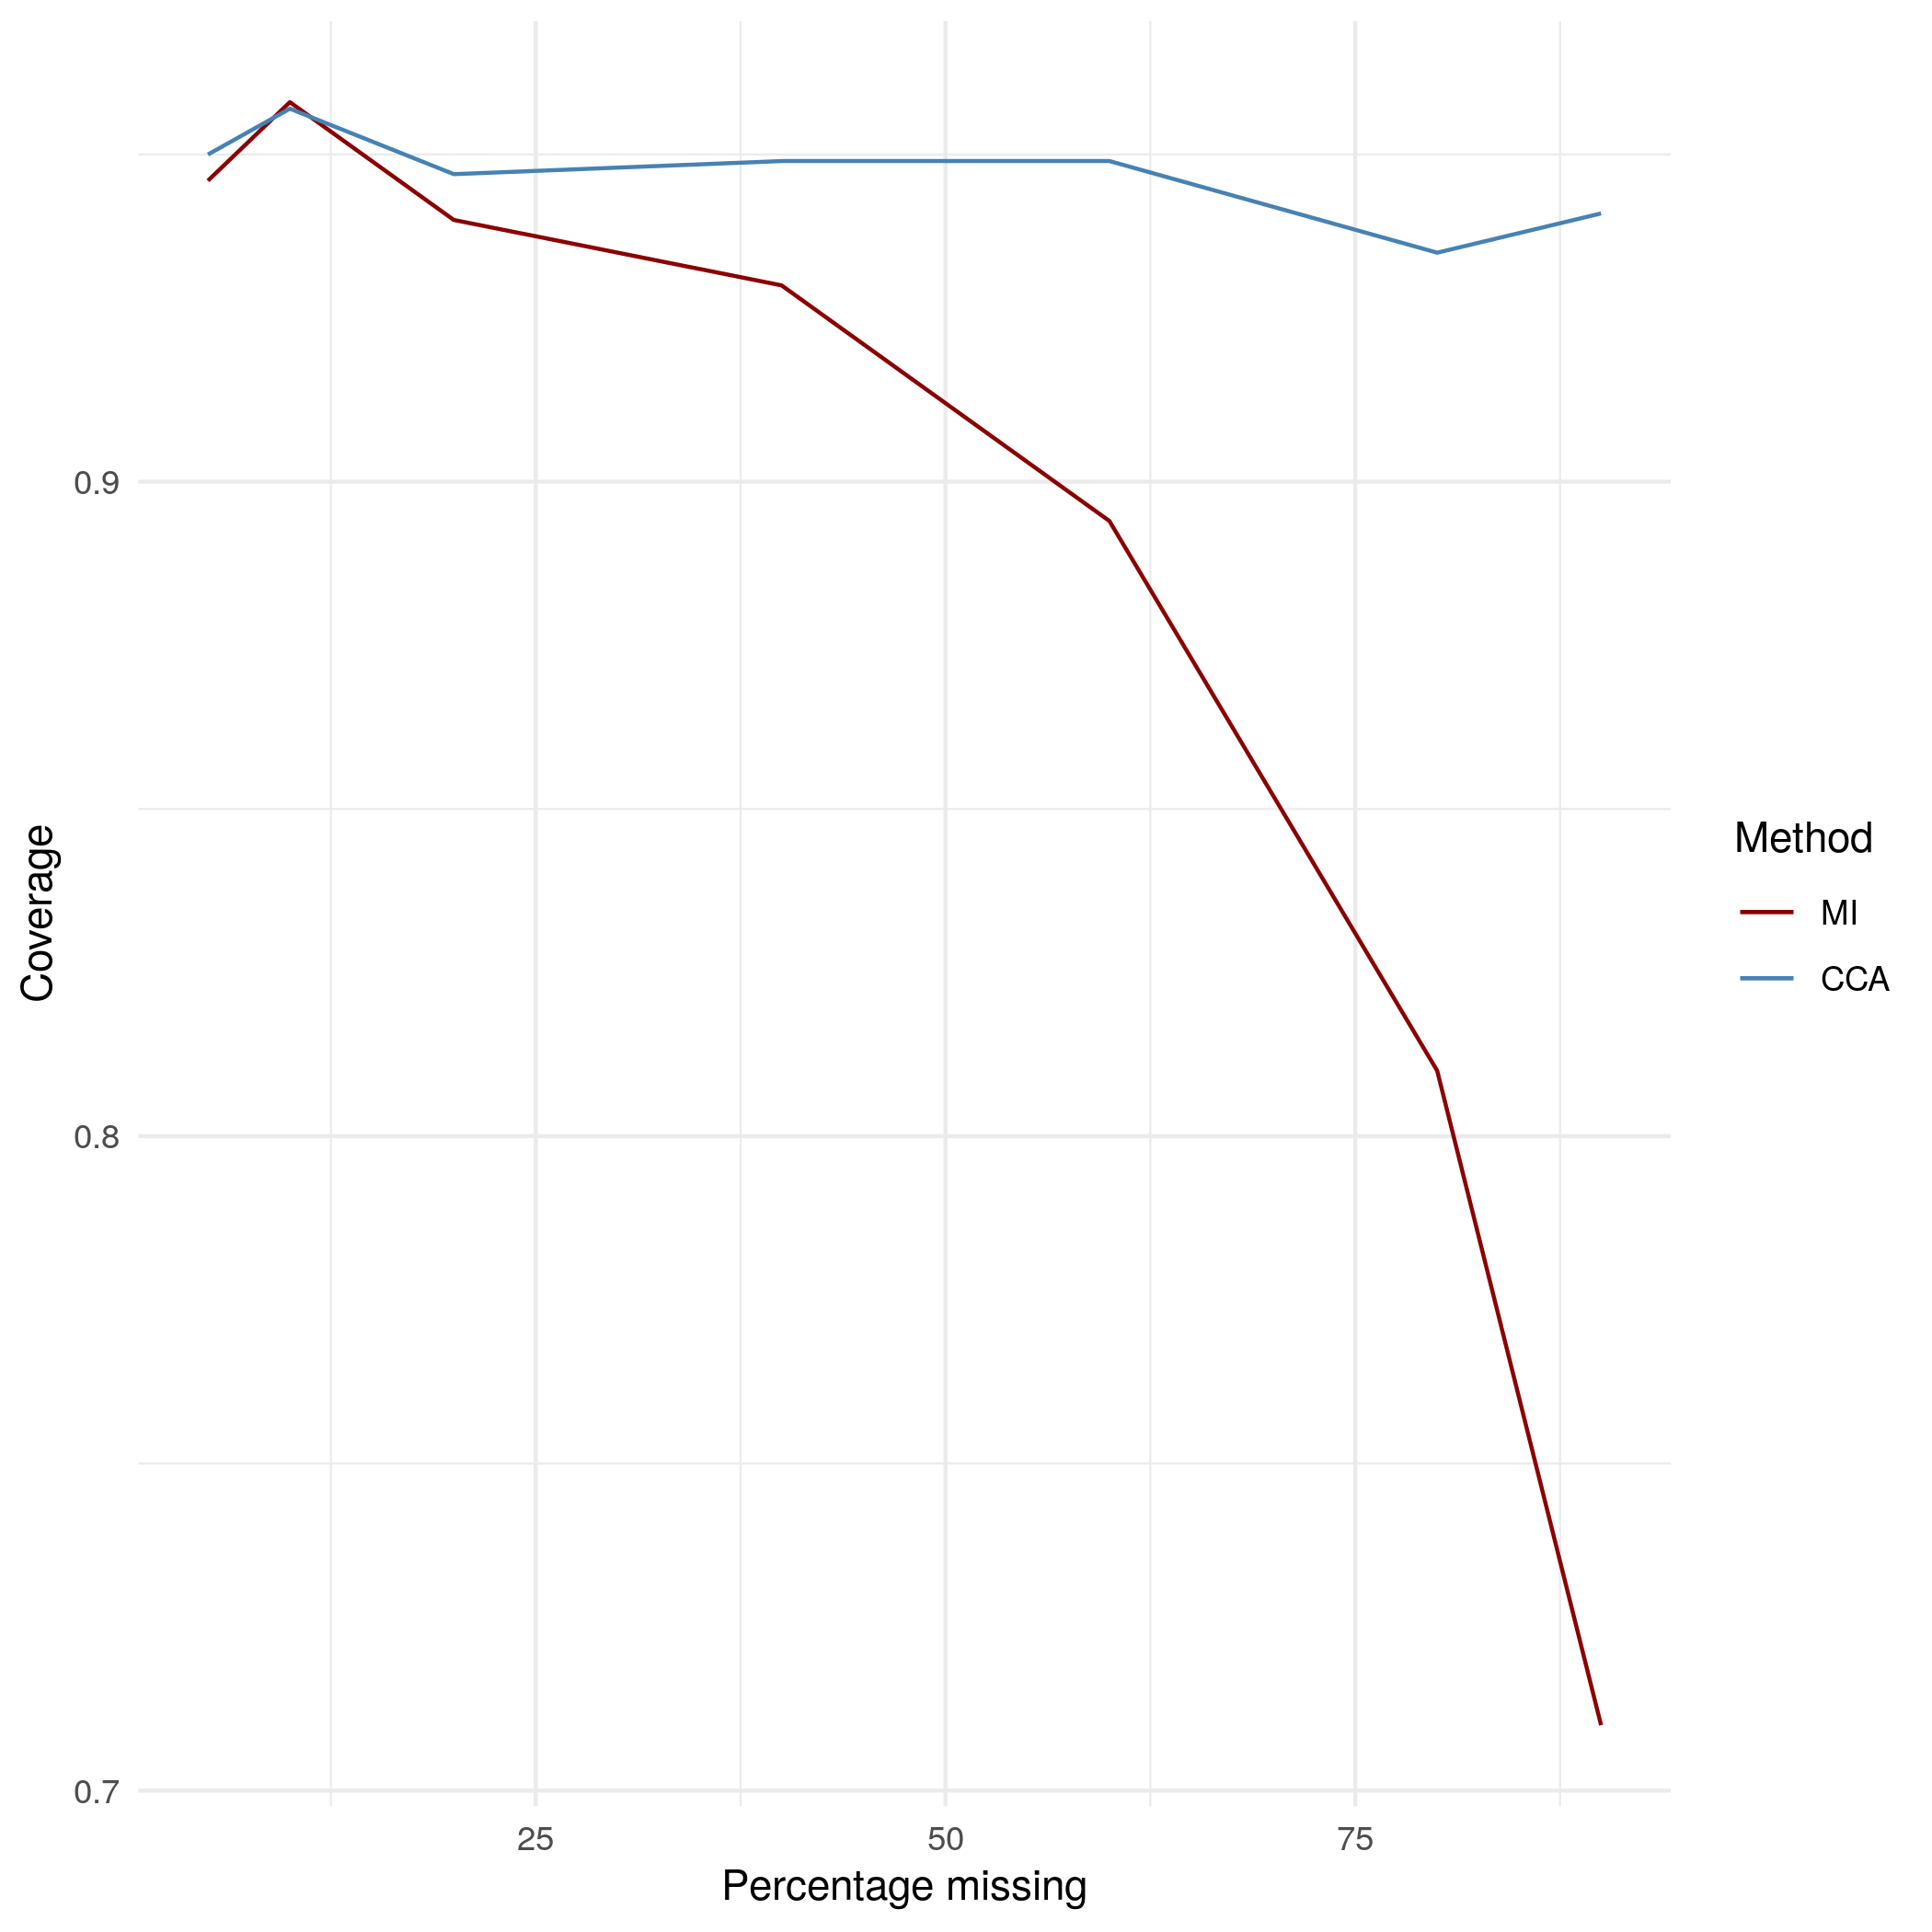
\includegraphics[width=0.3\textwidth]{mcar_coverage.png}}
		\quad
		\subfloat[Average CI size]{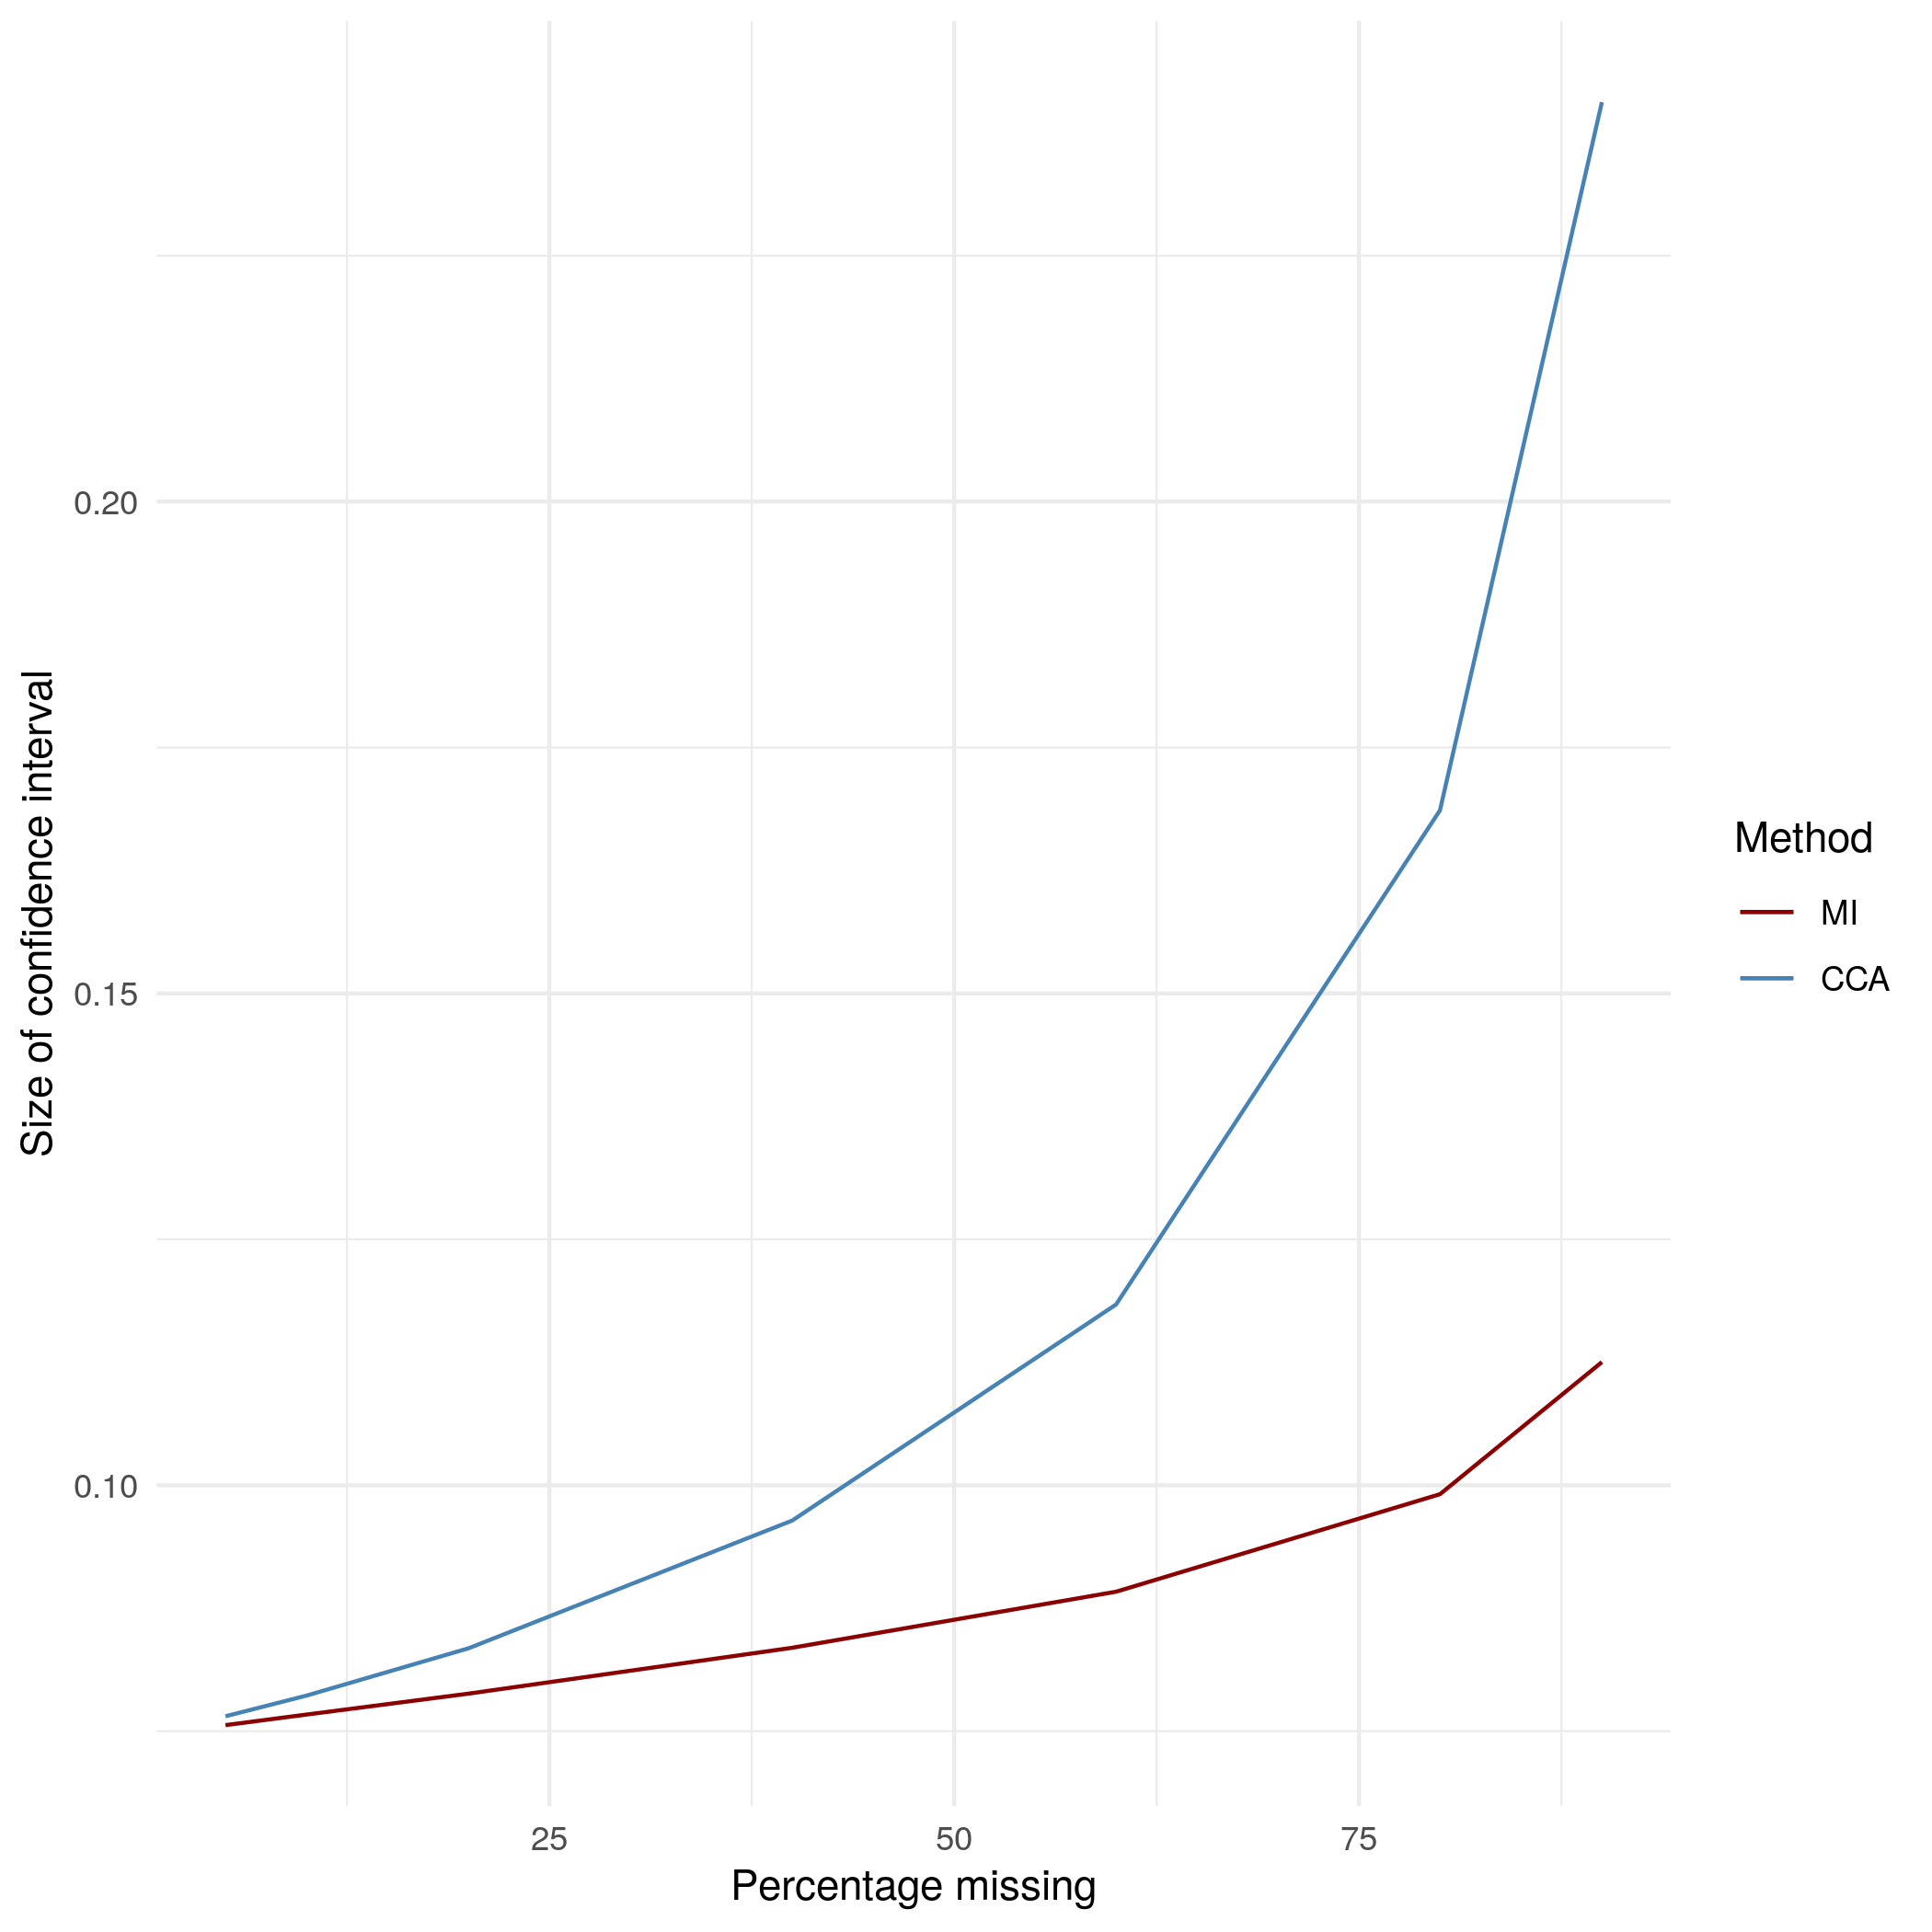
\includegraphics[width=0.3\textwidth]{mcar_ci.png}}
		\quad
		\subfloat[Average bias]{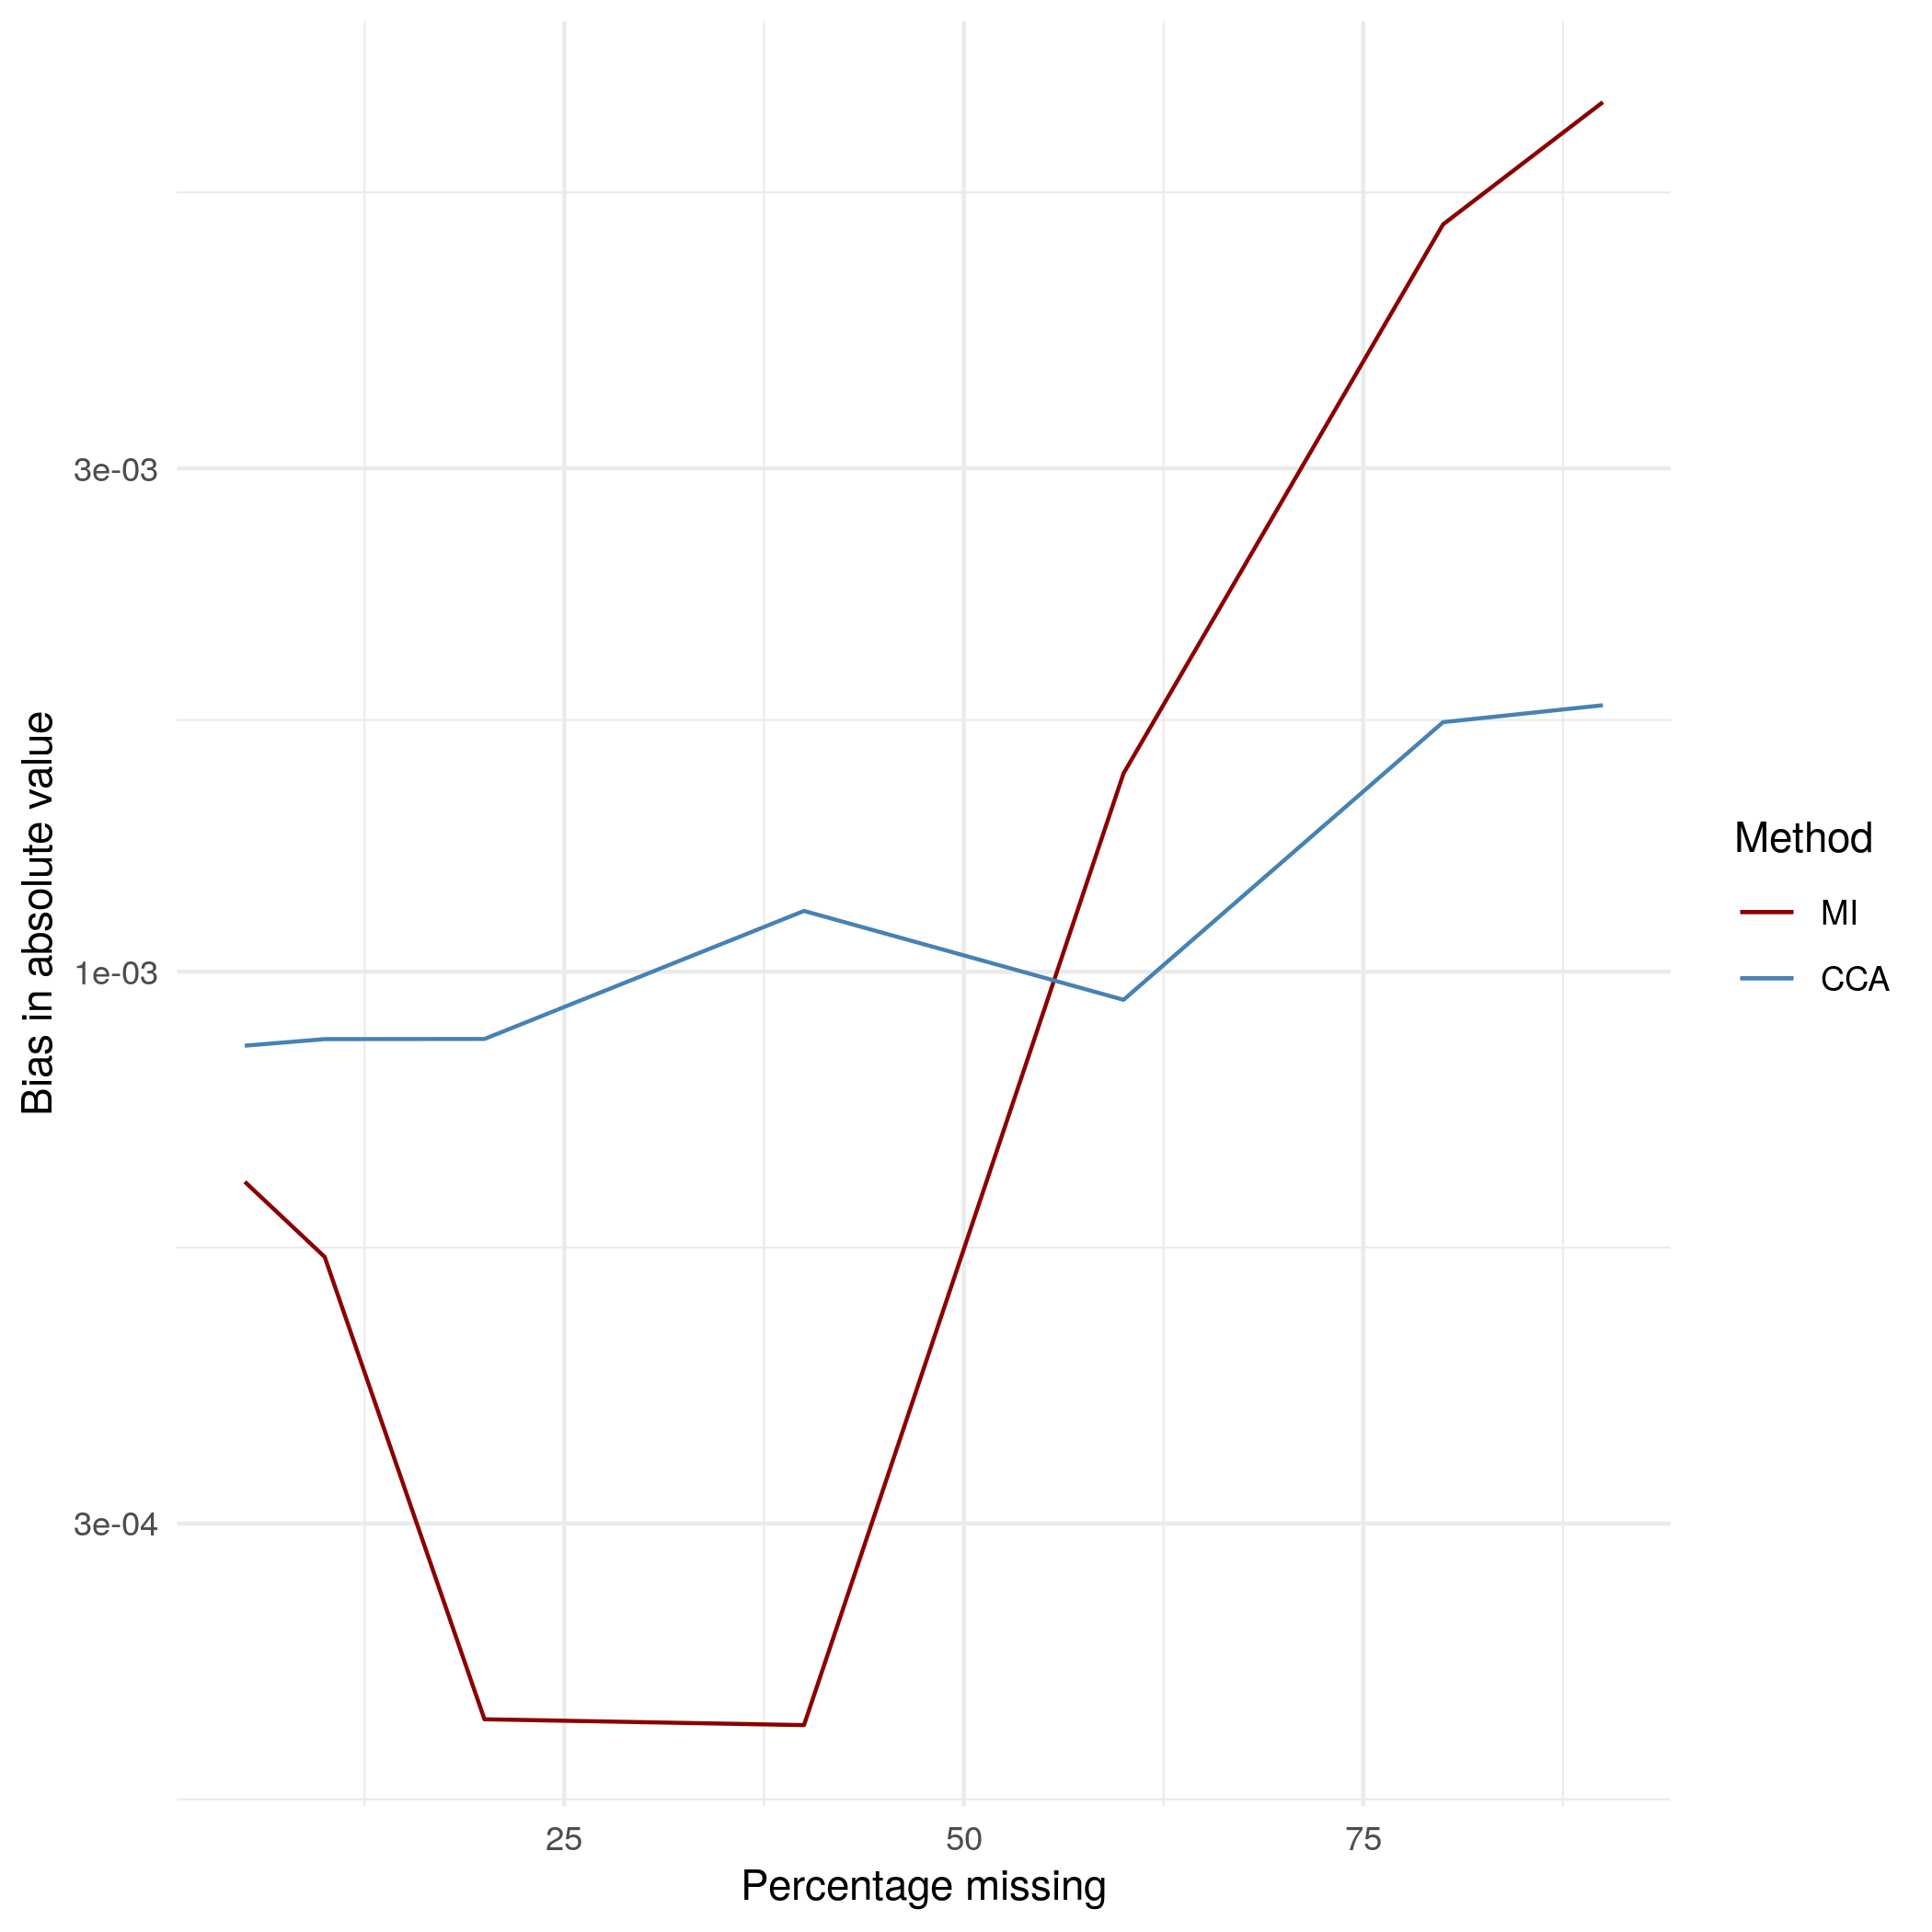
\includegraphics[width=0.3\textwidth]{mcar_bias.png}}
		\caption{Average results for MCAR missingness in $Y$ over 1000 repetitions of the analysis procedure described in 6.2.}
	\end{figure}
	
	Looking first at the $\beta_{1}$ estimates and their confidence intervals, we see that there is little difference between the methods other than the confidence interval of CCA growing at a much faster pace than that of MI as missingness increases. Next we observe that Bias is lower for MI at low missingness, while higher at high missingness. Additionally, coverage decreases substantially for MI as missingness increases.
	
	Overall it seems like MI provides some benefit over CCA in a low missingness scenario, while CCA seems superior otherwise. The poor performance of MI at higher amounts of missingness suggests an instability in the implementation, whether in MICE or the supplementary code. Another possibility is that at 90 percent missingness our estimates for the conditional distribution of $Y$ become too inaccurate.
	
	\subsubsection{MAR}

	\begin{figure}[H]
		\centering
		\subfloat[$\beta_{1}$ estimate with CCA]{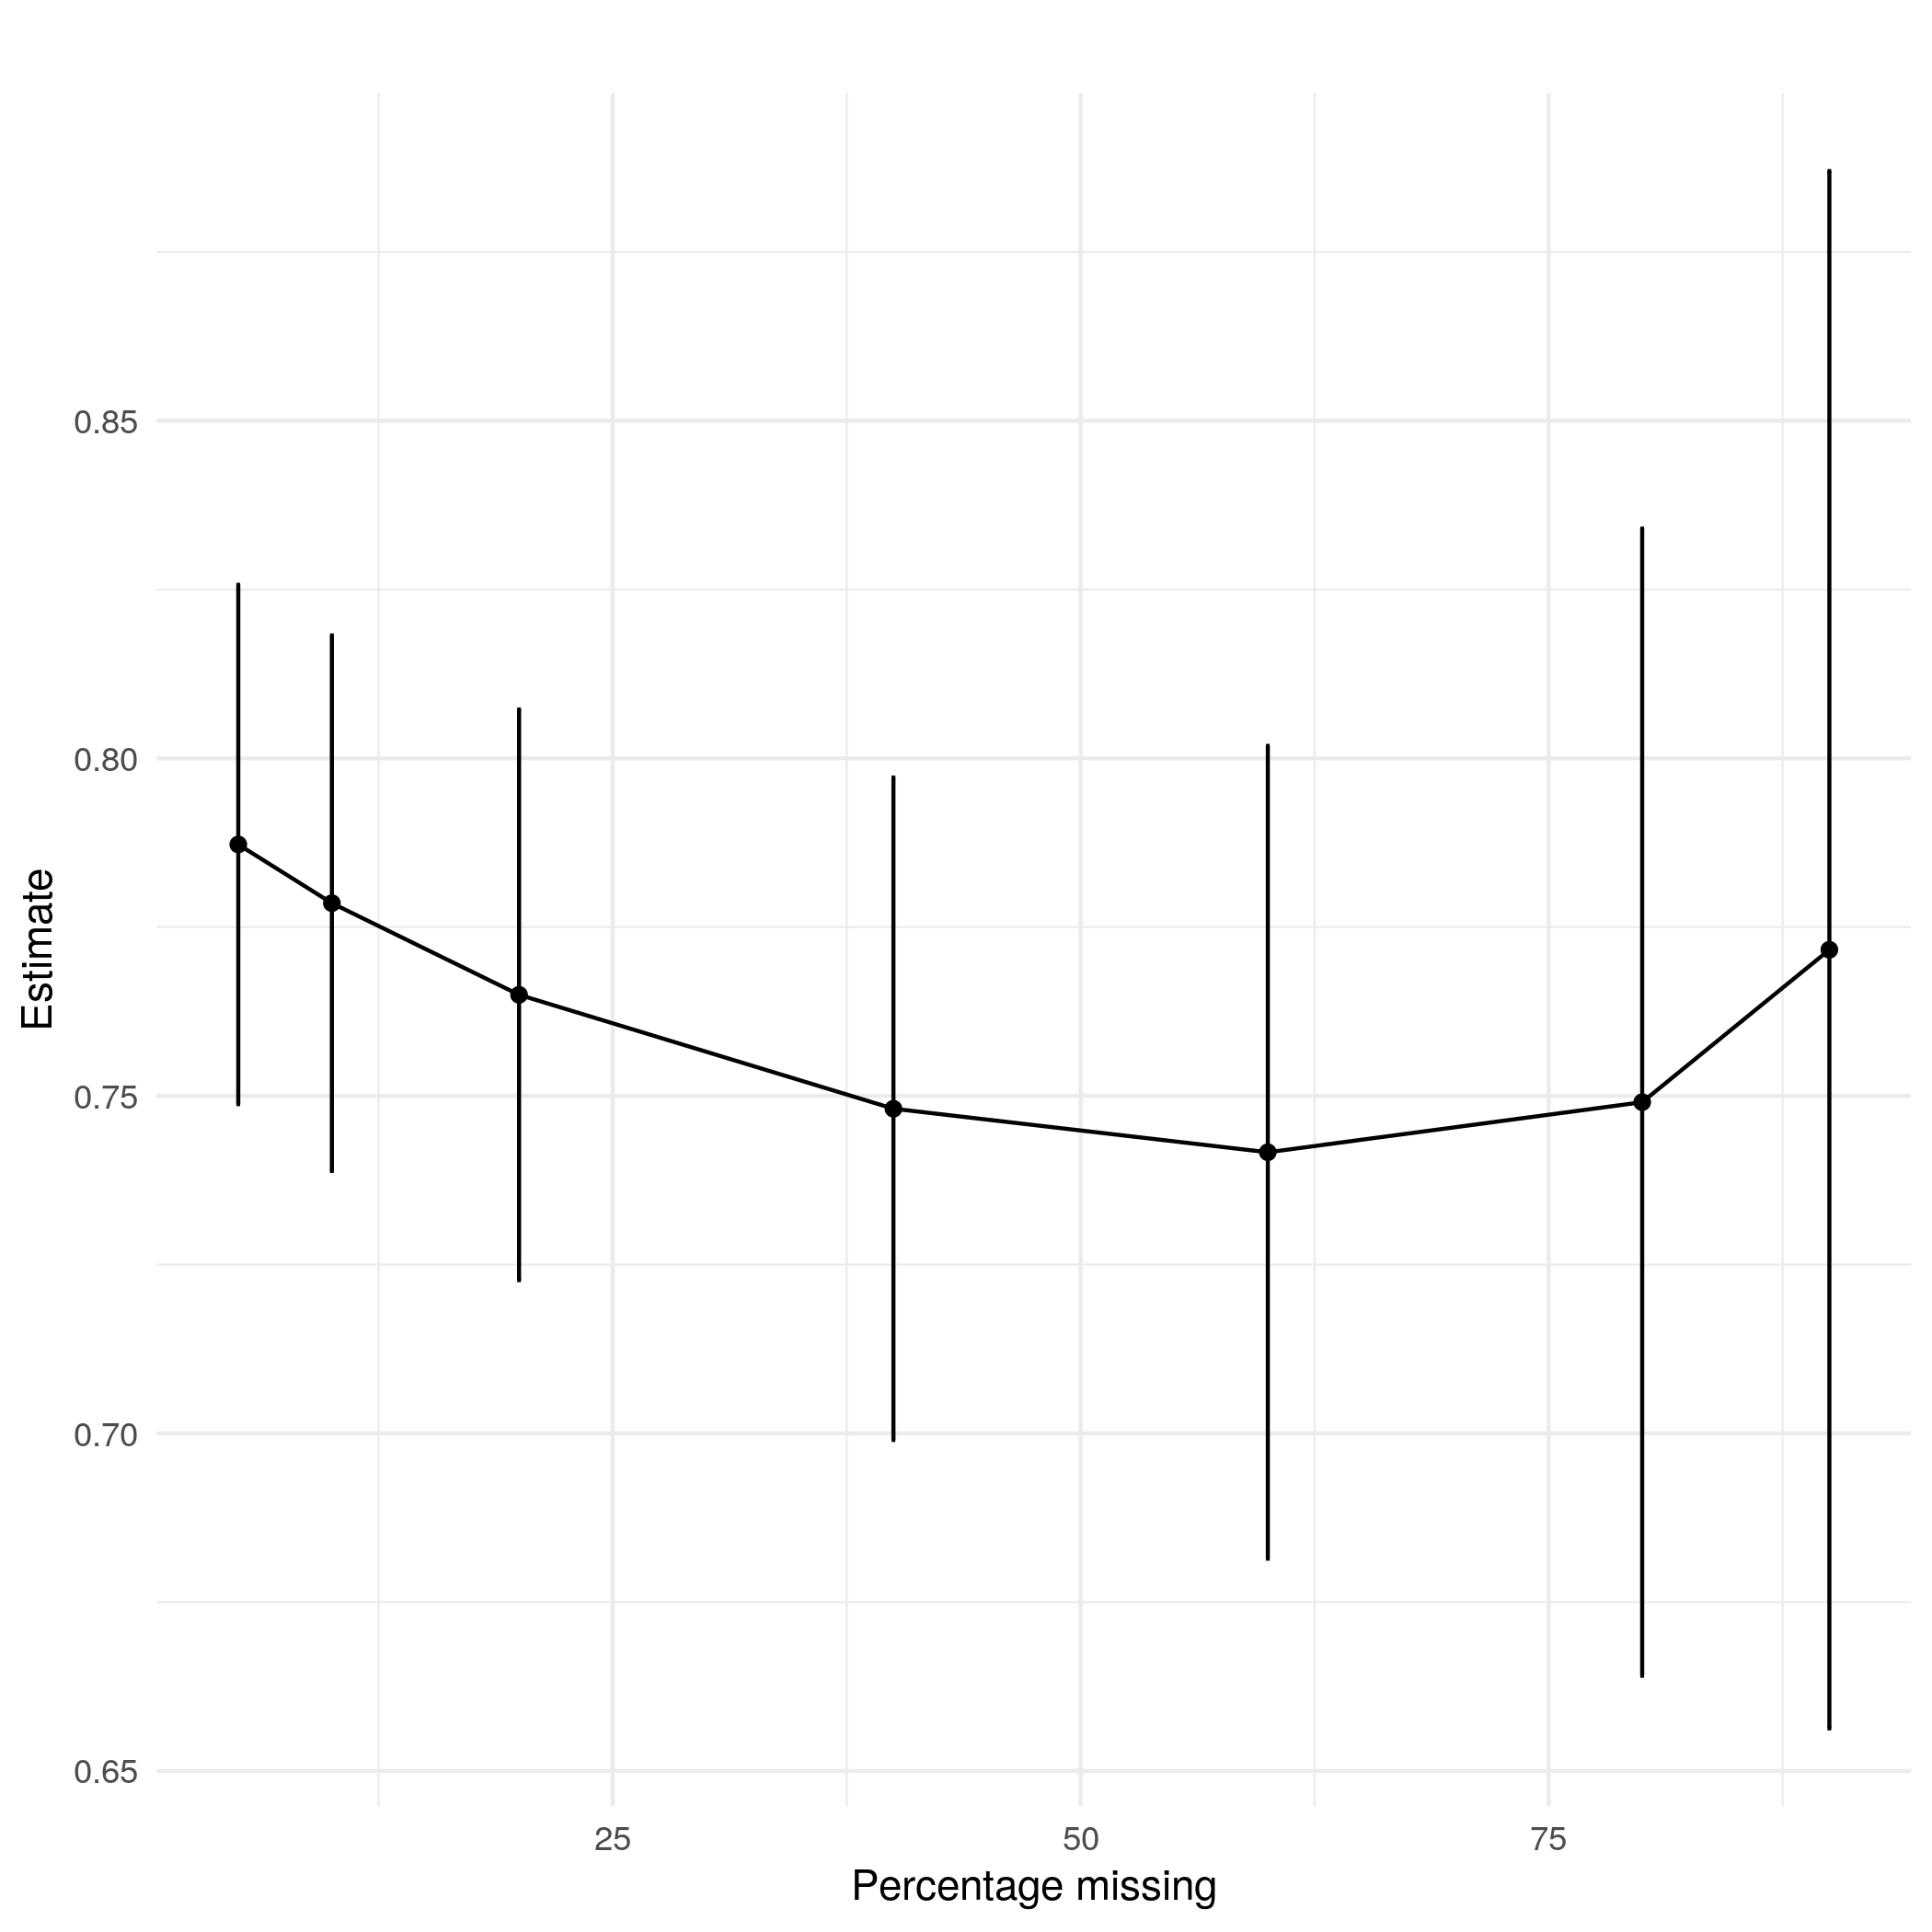
\includegraphics[width=0.4\textwidth]{mar_reg_x_estimate_cca.png}}
		\quad
		\subfloat[$\beta_{1}$ estimate with MI]{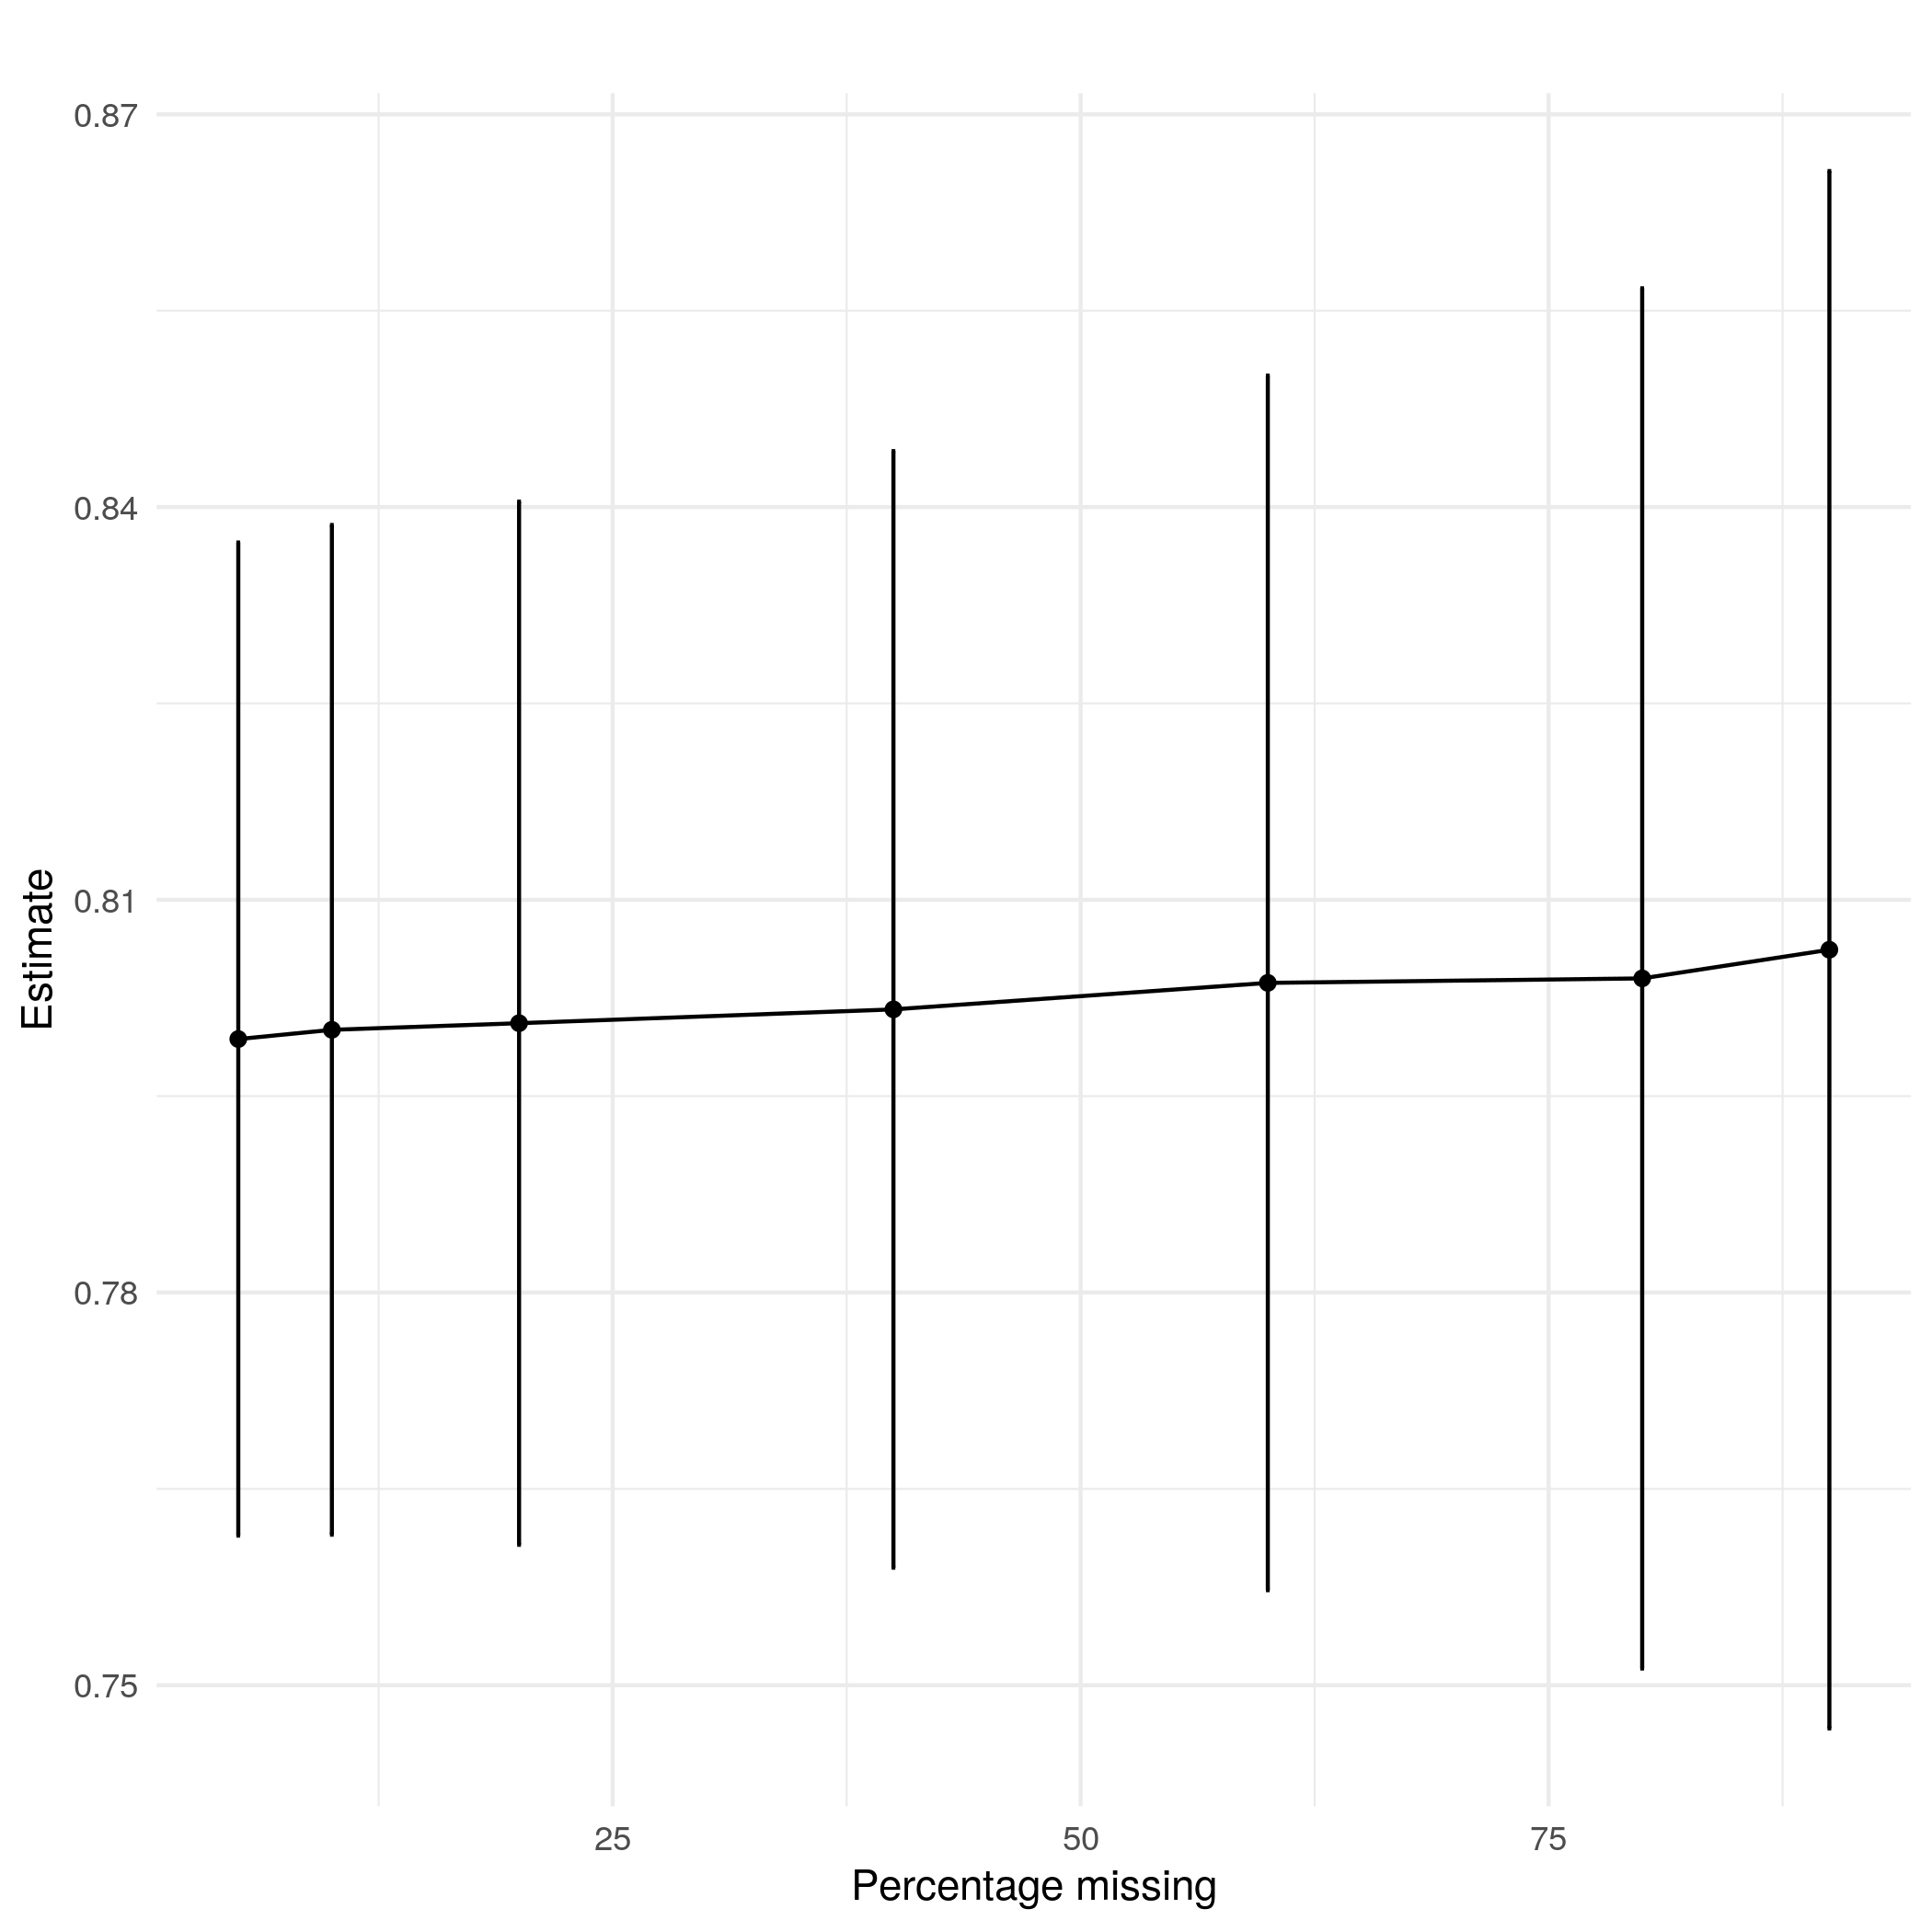
\includegraphics[width=0.4\textwidth]{mar_reg_x_estimate_mi.png}}
		\\
		\subfloat[Coverage]{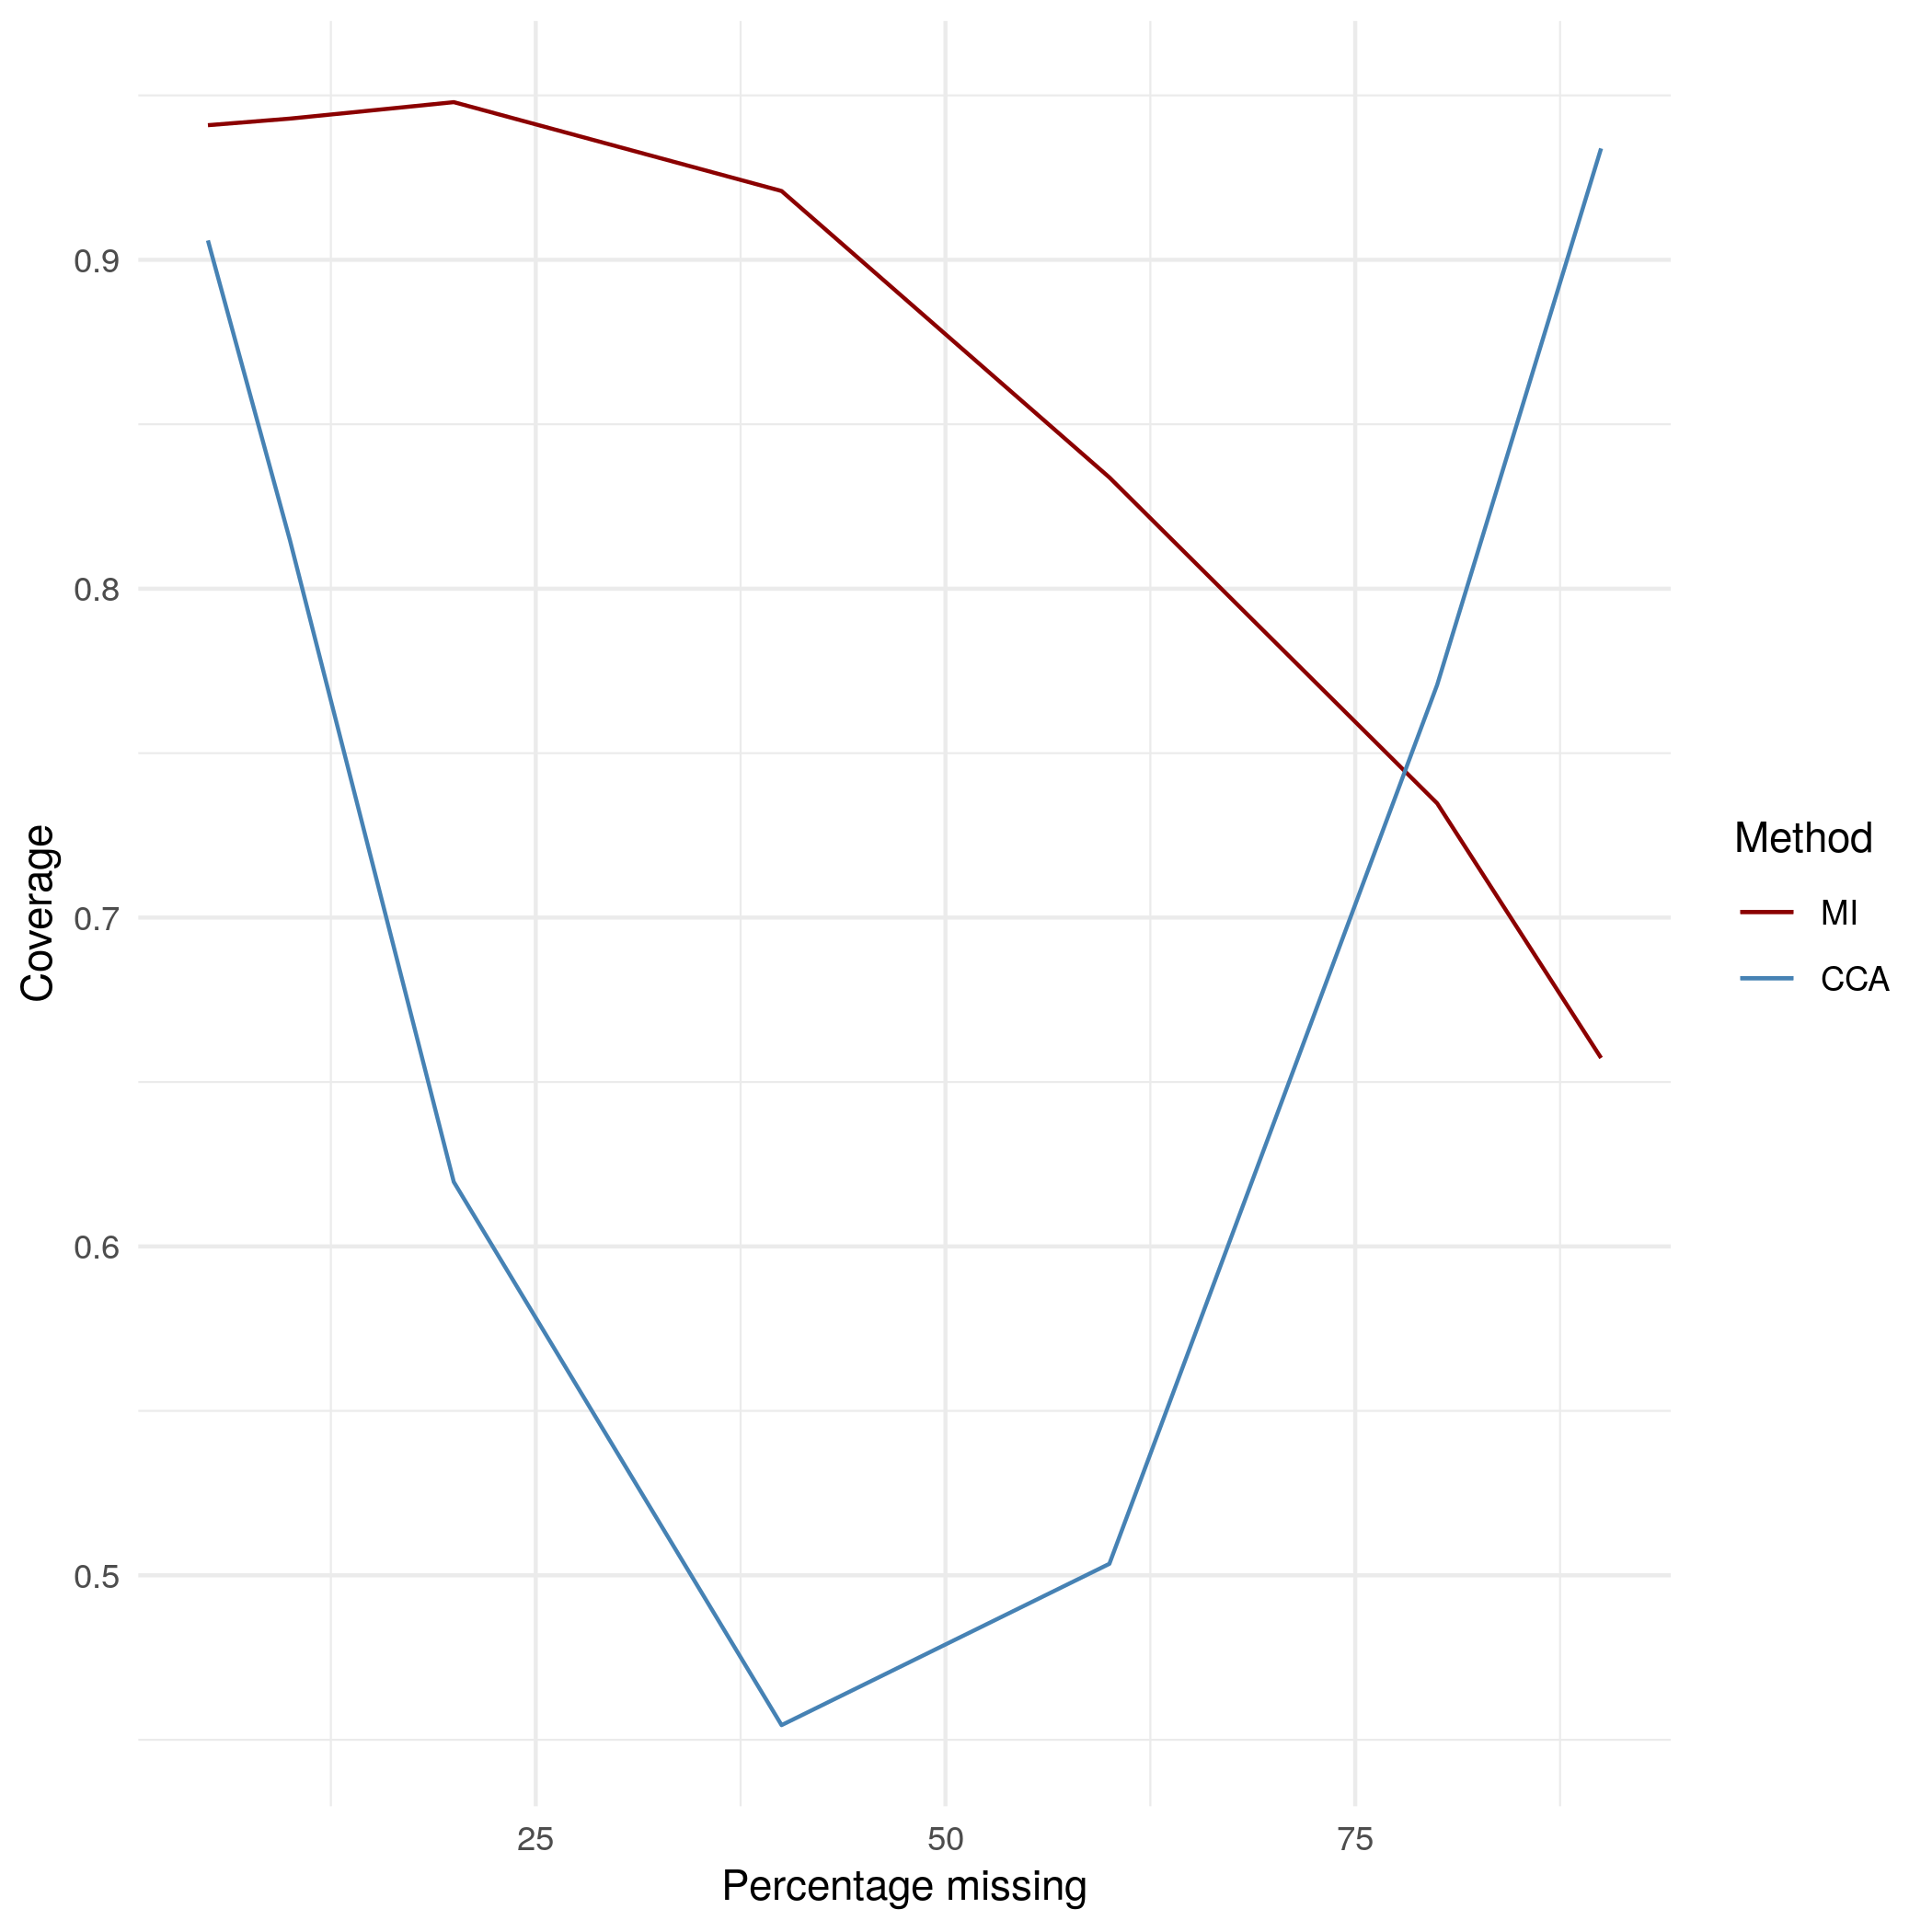
\includegraphics[width=0.3\textwidth]{mar_reg_x_coverage.png}}
		\quad
		\subfloat[Average CI size]{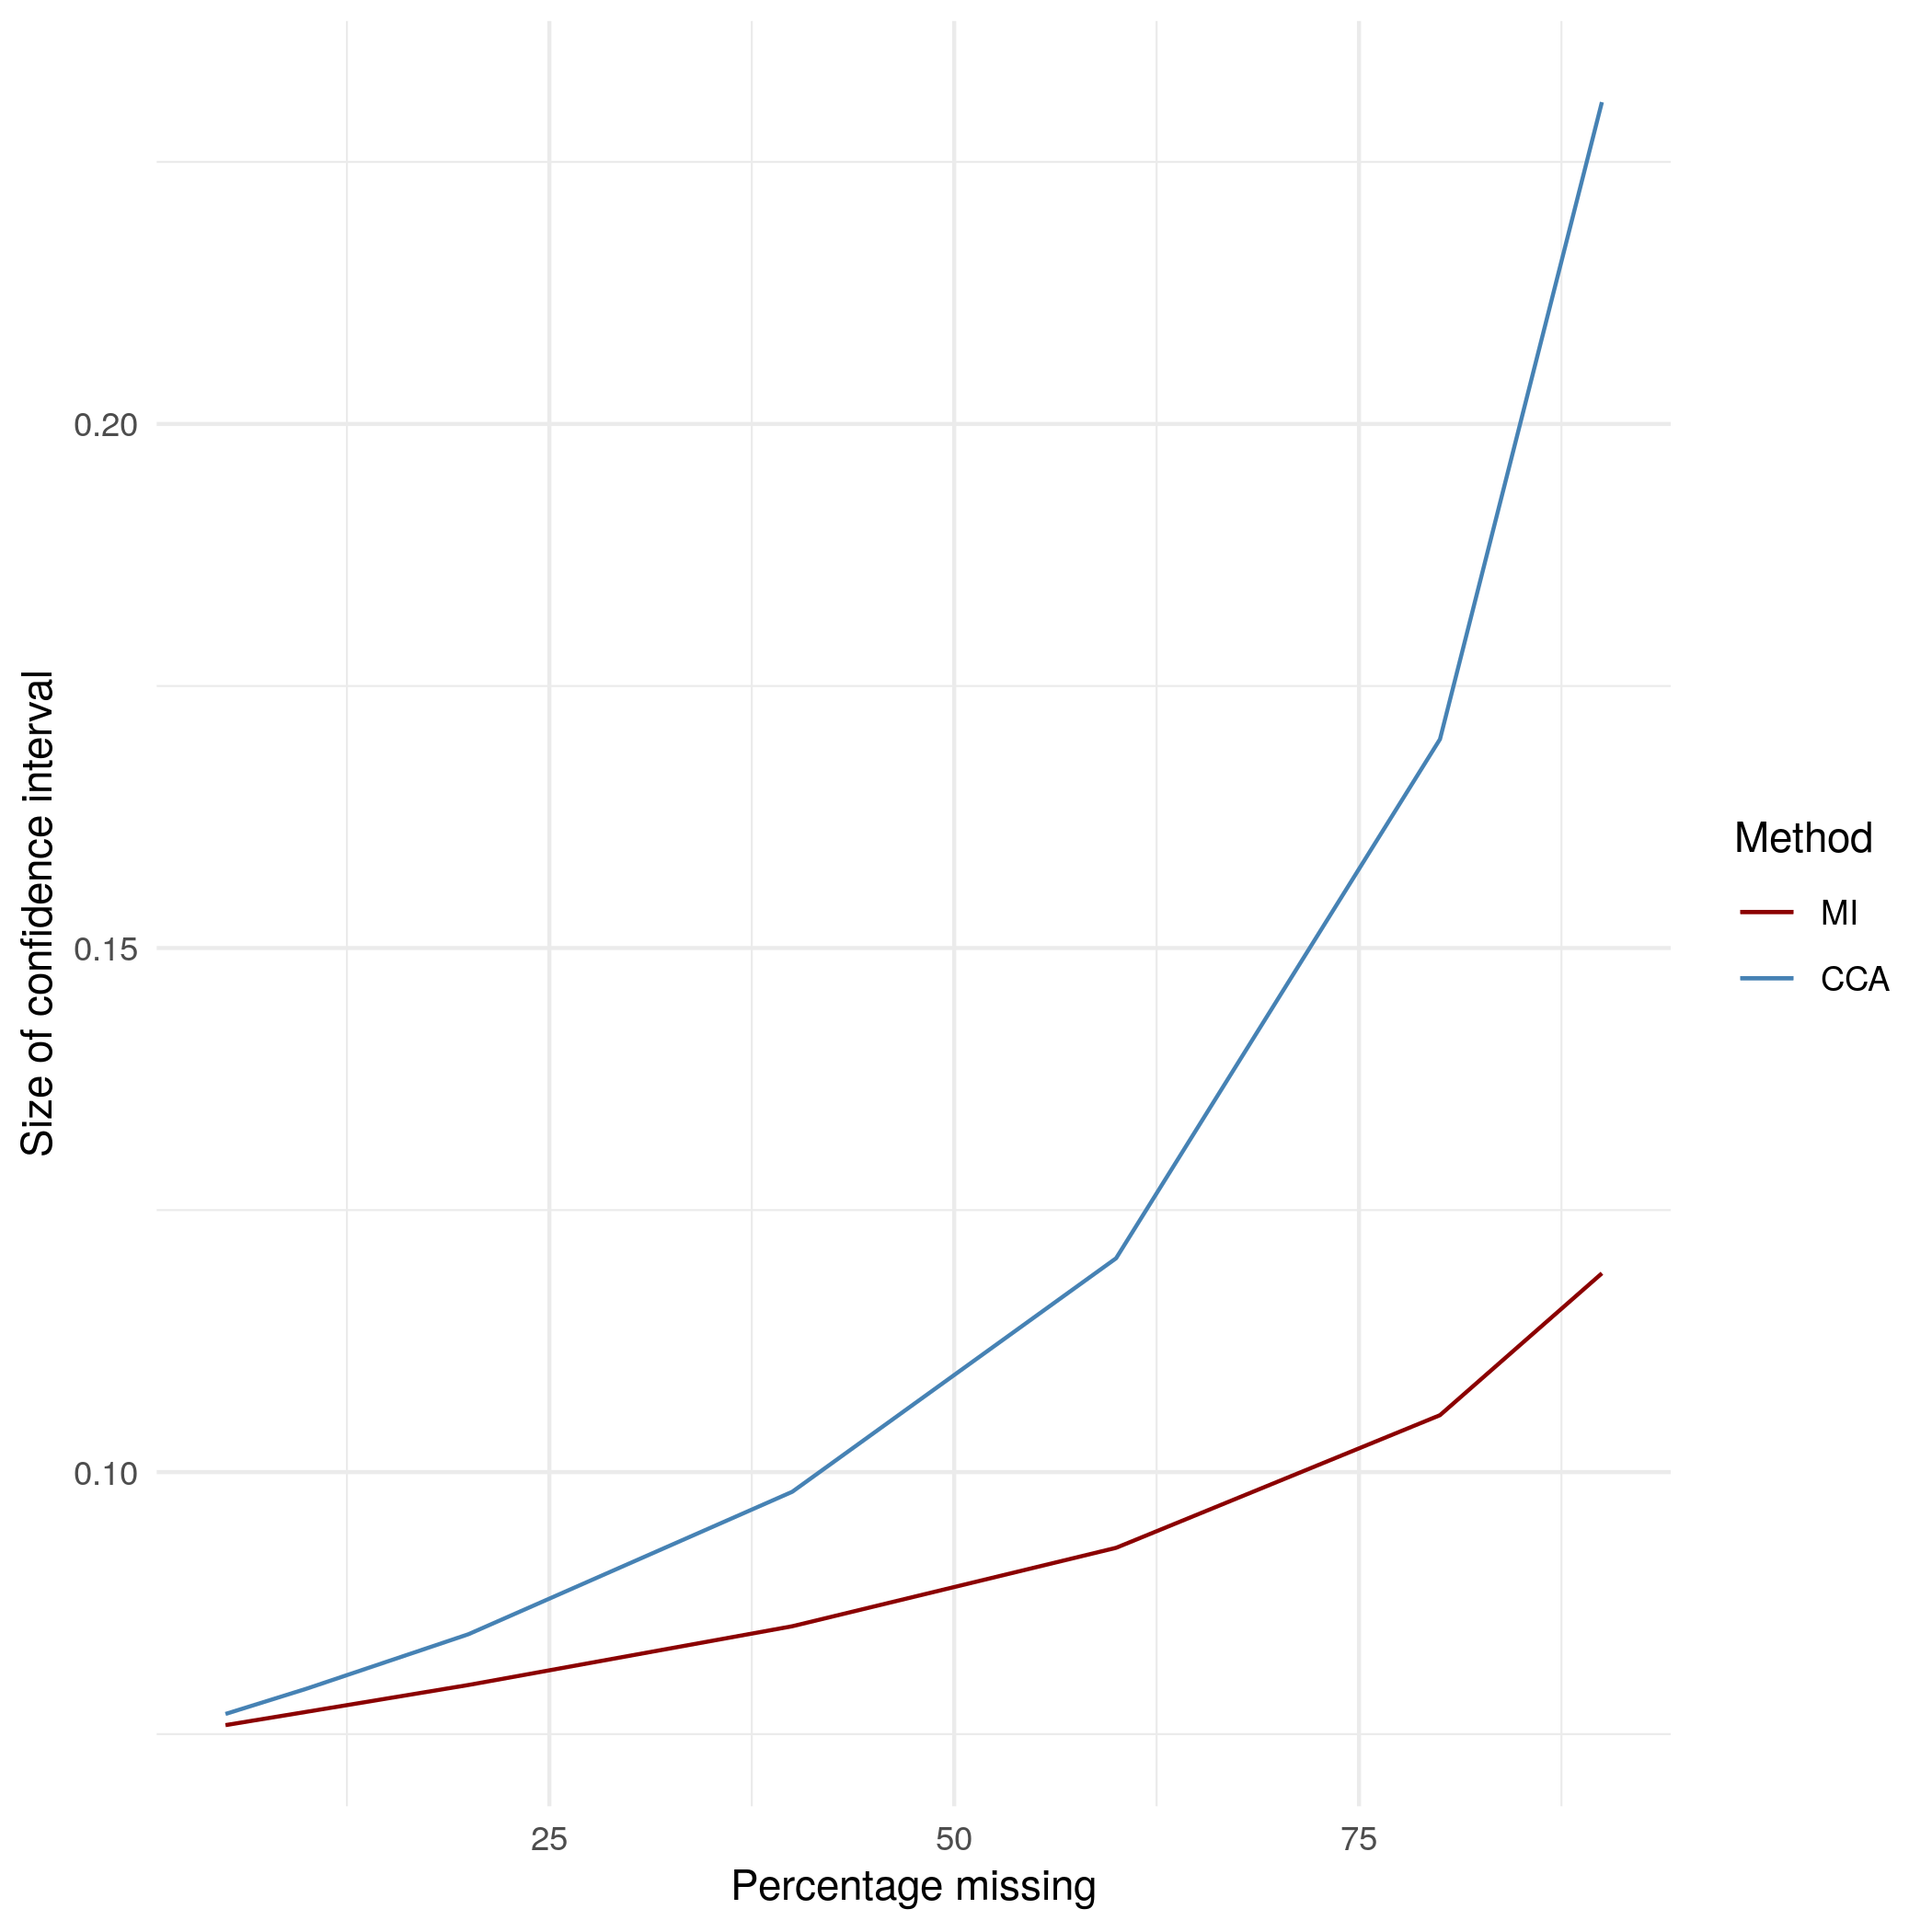
\includegraphics[width=0.3\textwidth]{mar_reg_x_ci.png}}
		\quad
		\subfloat[Average bias]{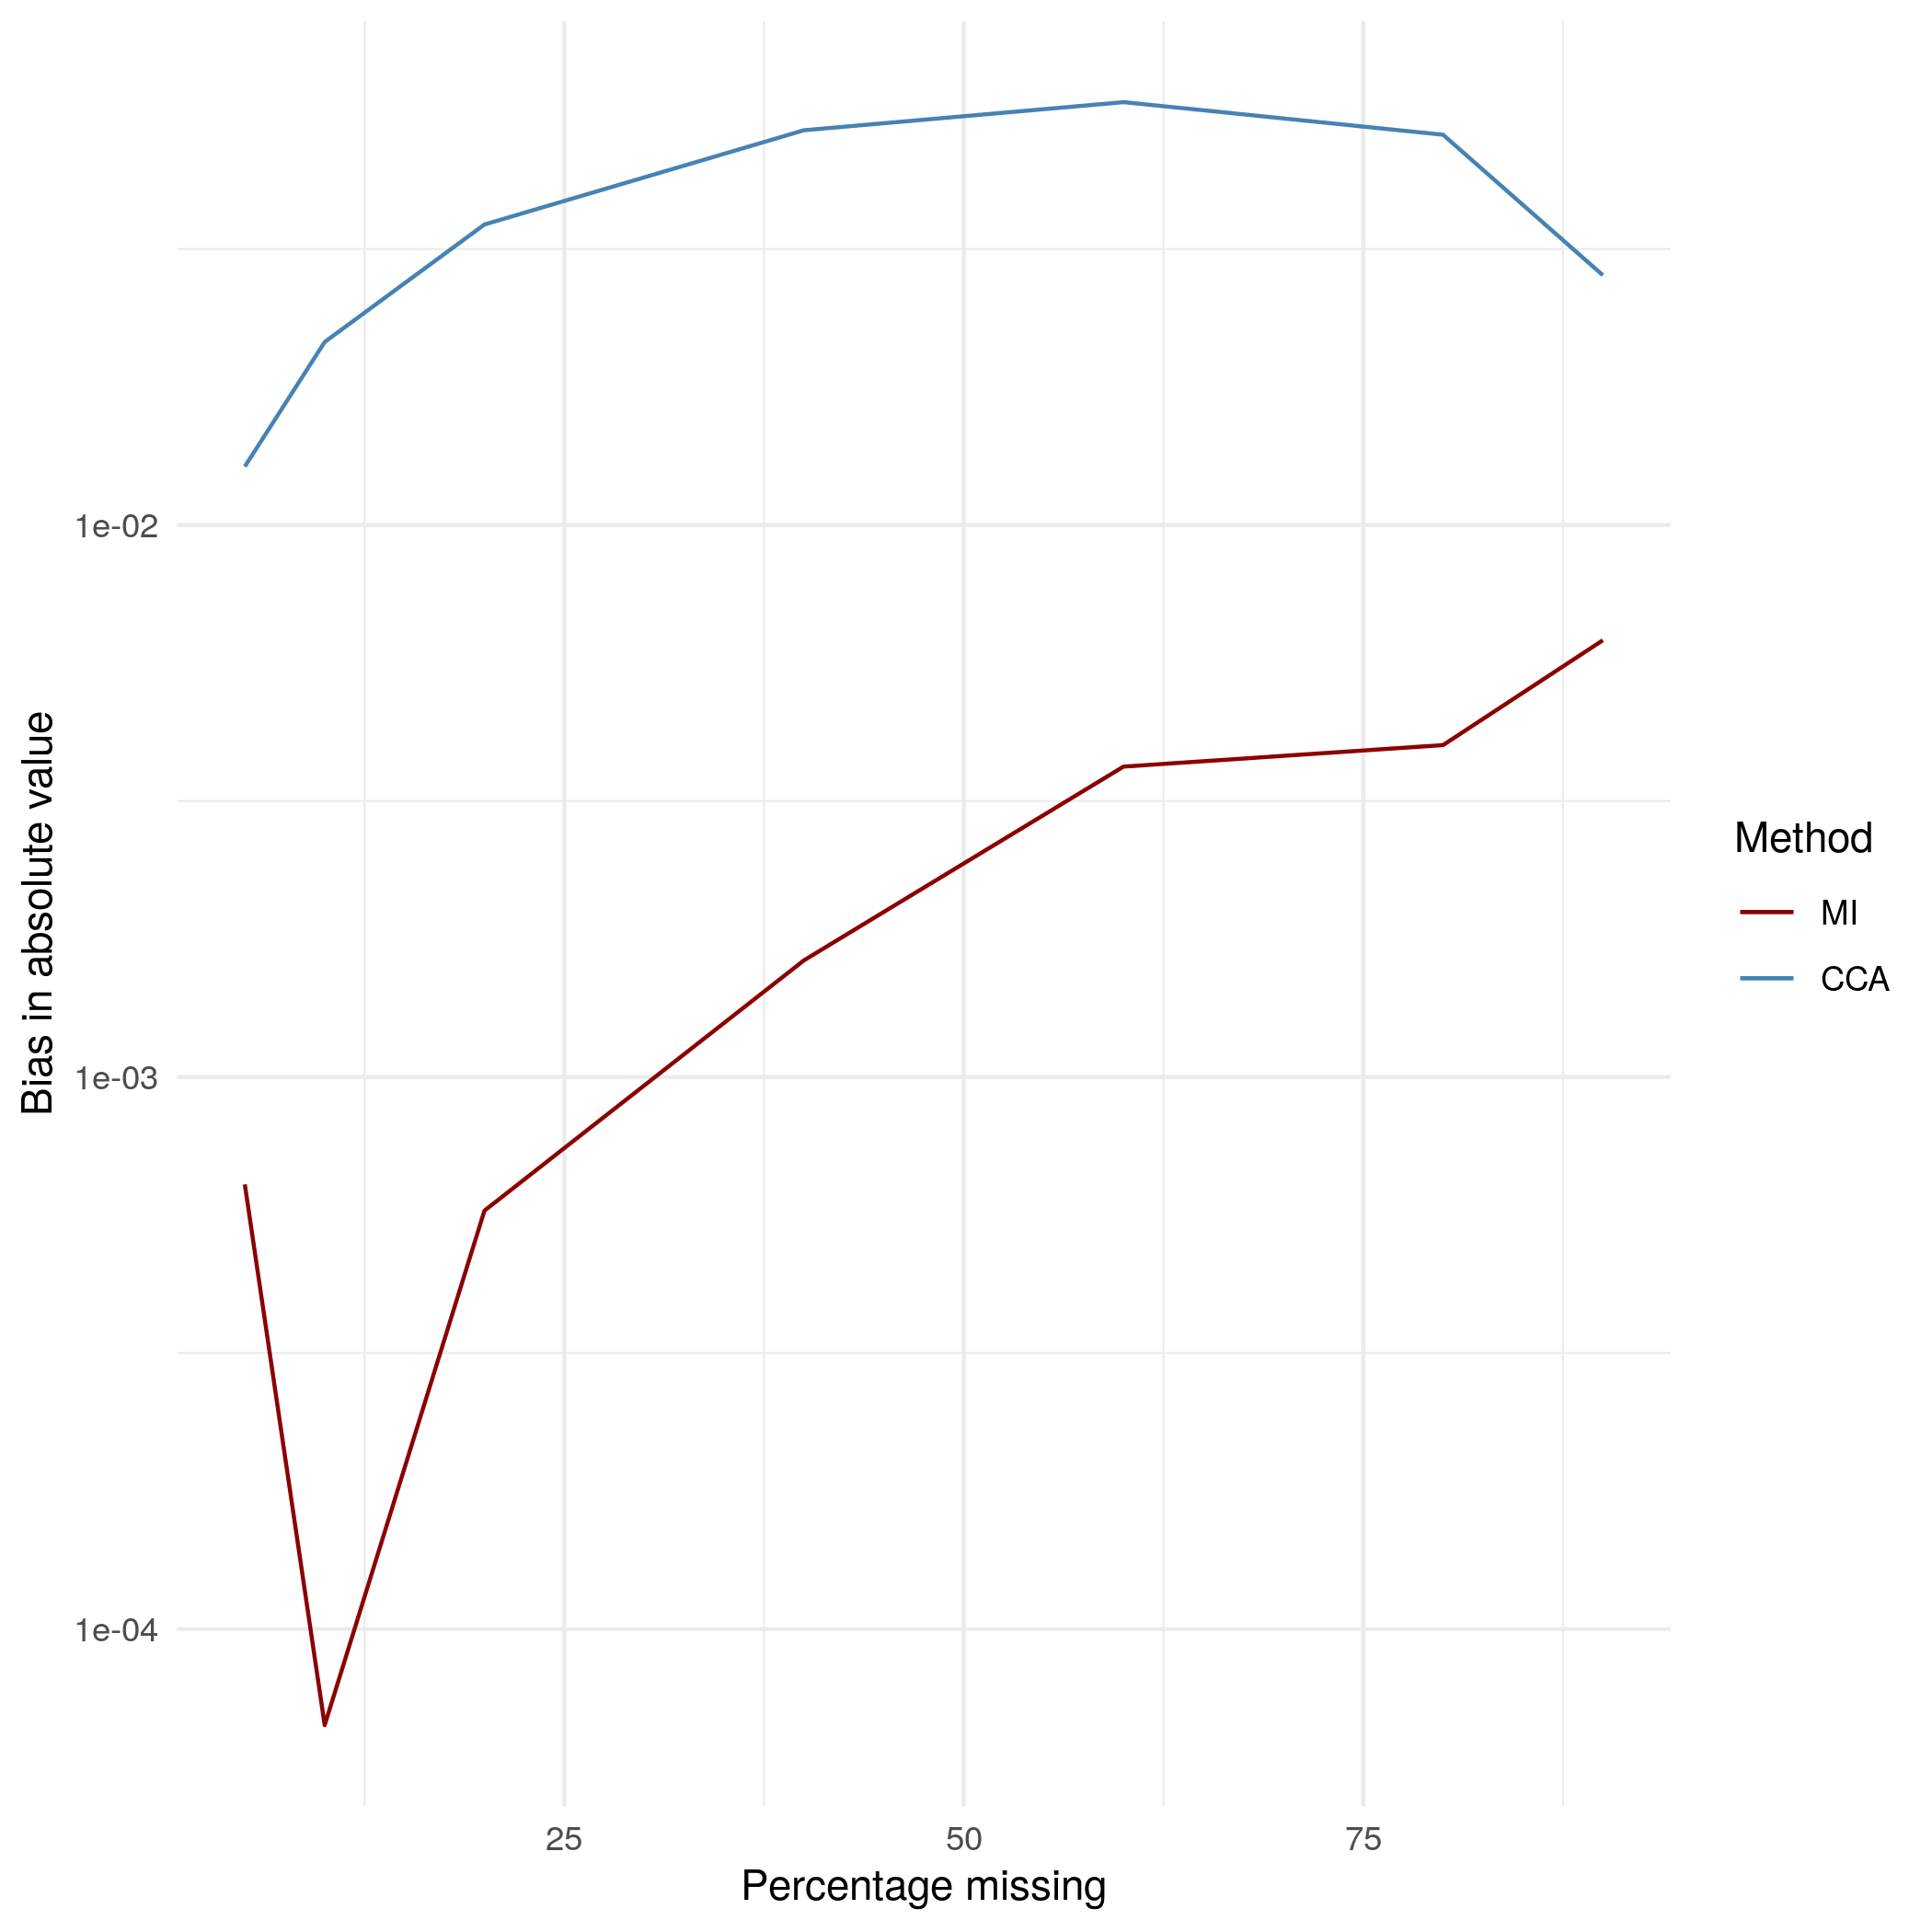
\includegraphics[width=0.3\textwidth]{mar_reg_x_bias.png}}
		\caption{Average results for MAR missingness in $X$ over 1000 repetitions of the analysis procedure described in 6.2.}
	\end{figure}
	For missingness in $X$ we find that MI provides substantial benefits in reducing bias and increasing coverage while at the same time reducing the size of confidence intervals. This is in line with earlier theory and results described in literature.
	
	\begin{figure}[H]
		\centering
		\subfloat[$\beta_{1}$ estimate with CCA]{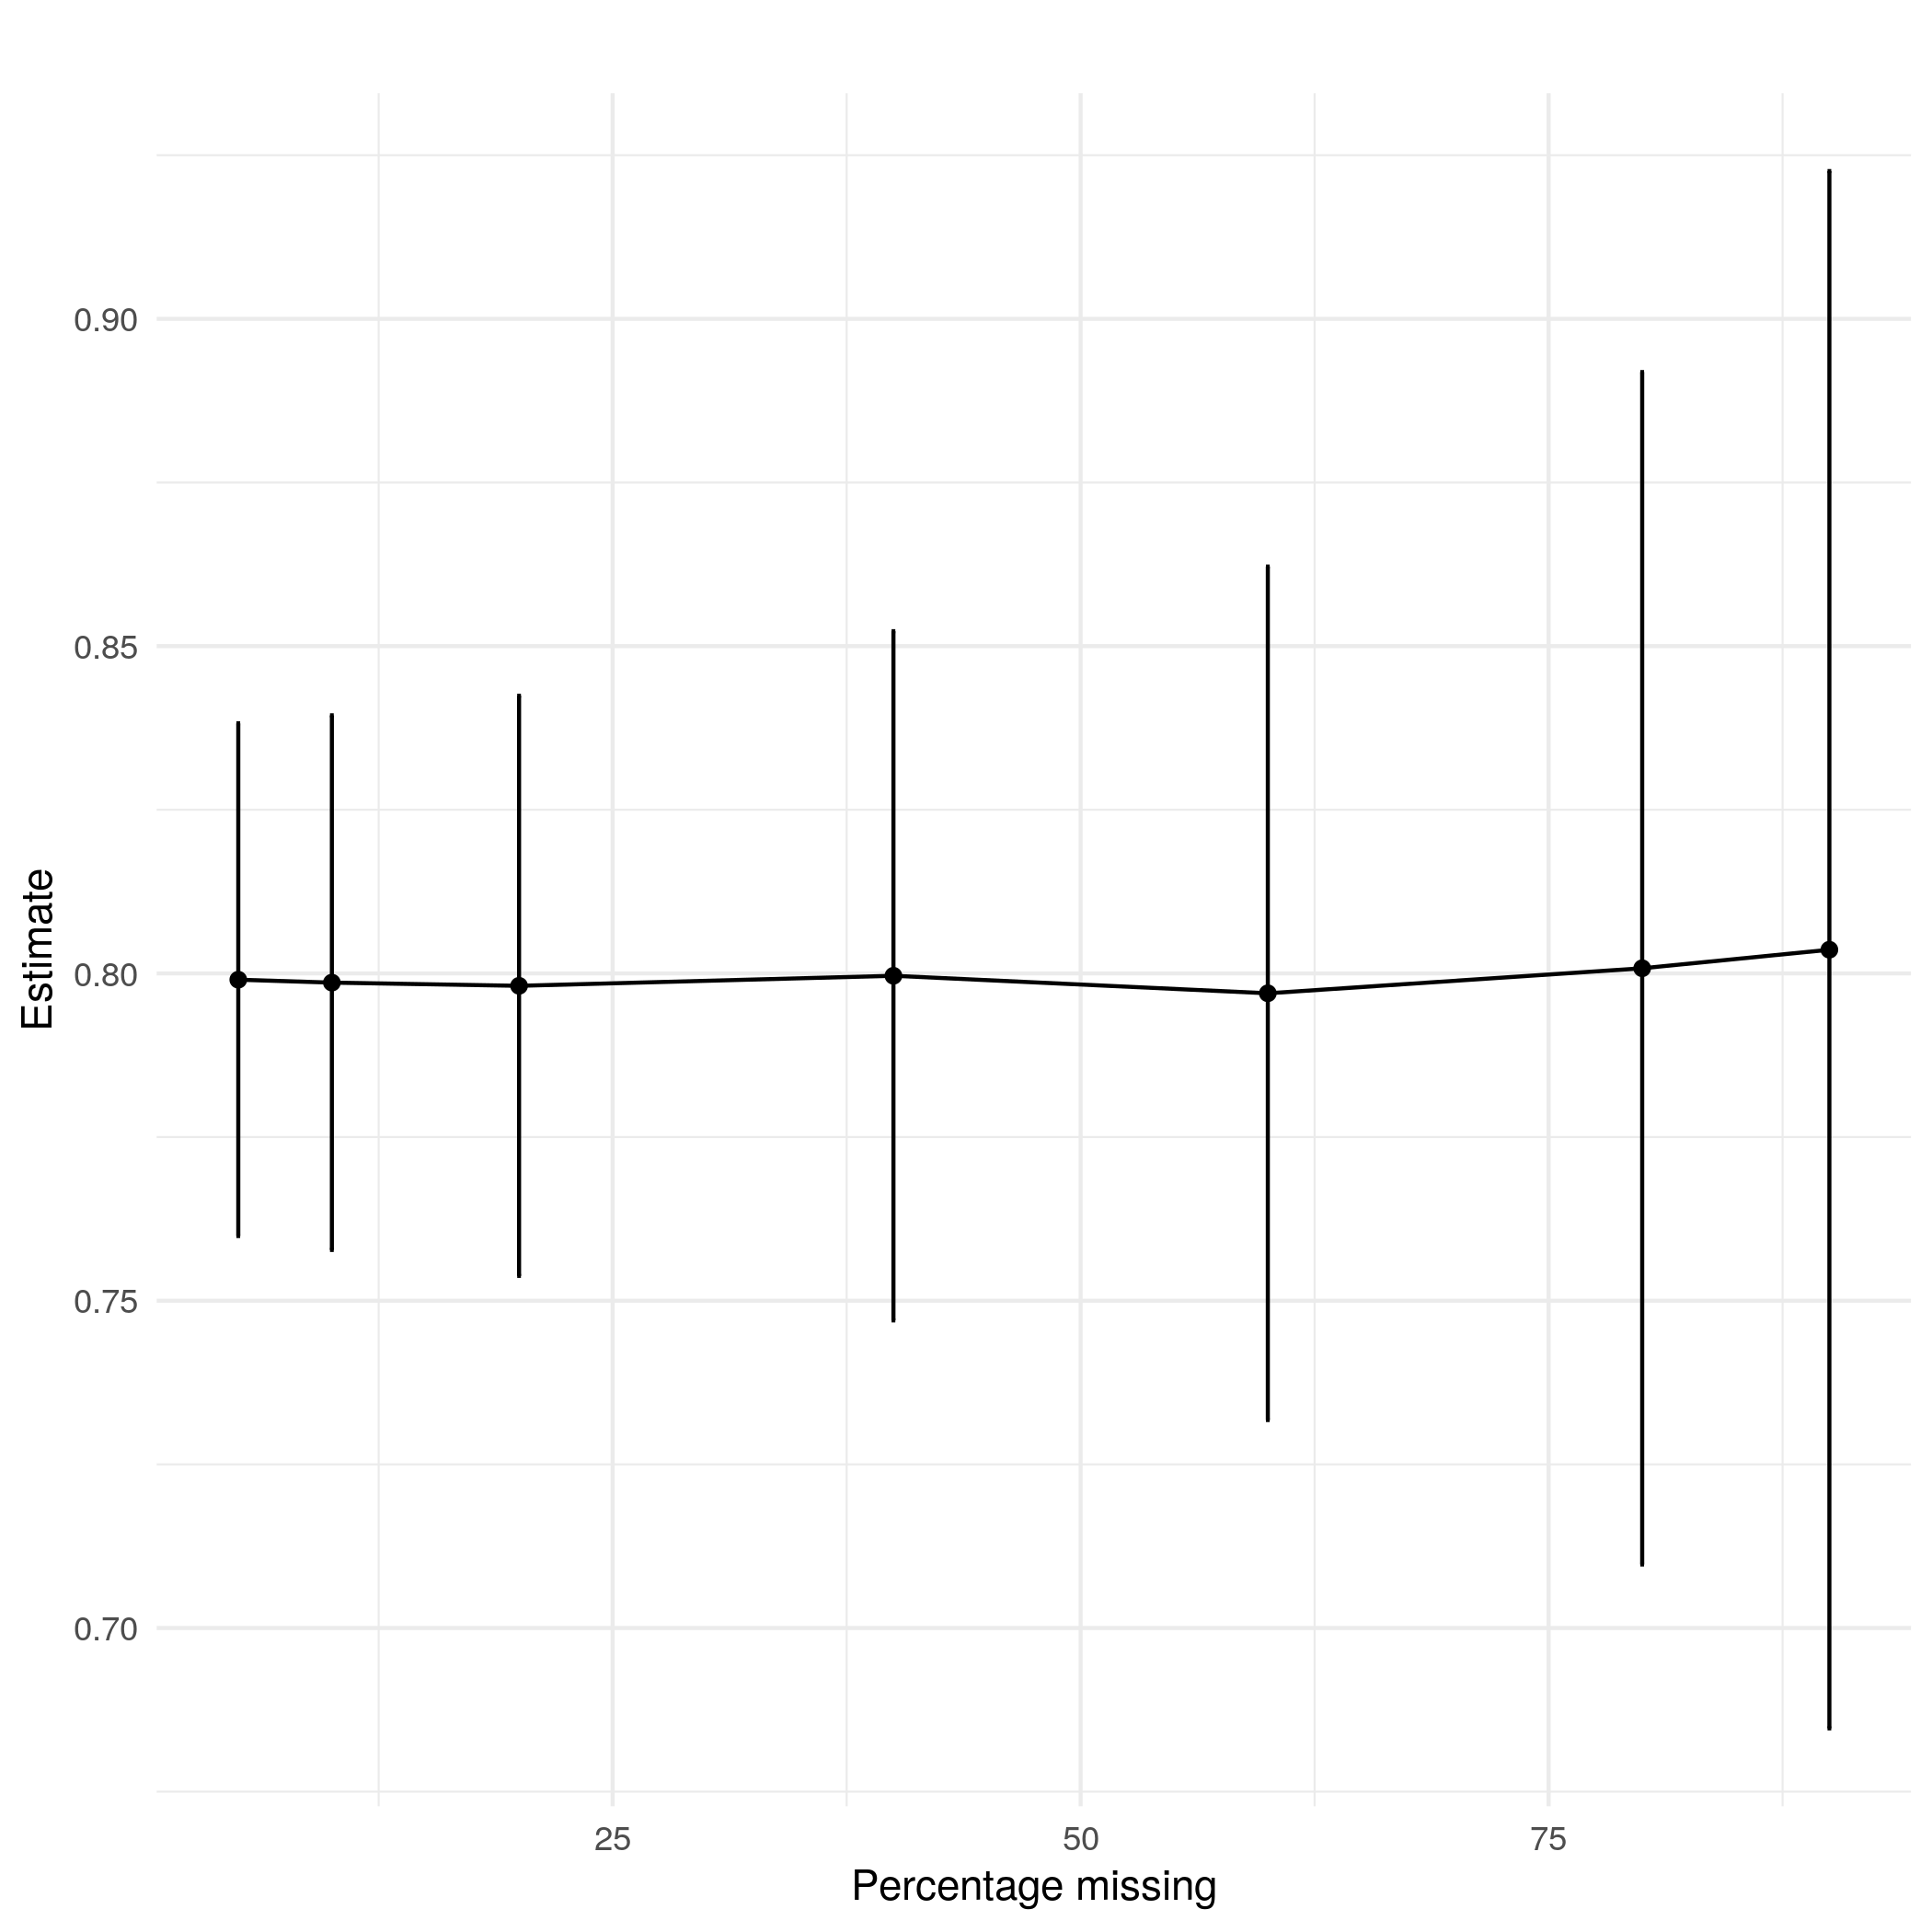
\includegraphics[width=0.4\textwidth]{final_estimate_cca.png}}
		\quad
		\subfloat[$\beta_{1}$ estimate with MI]{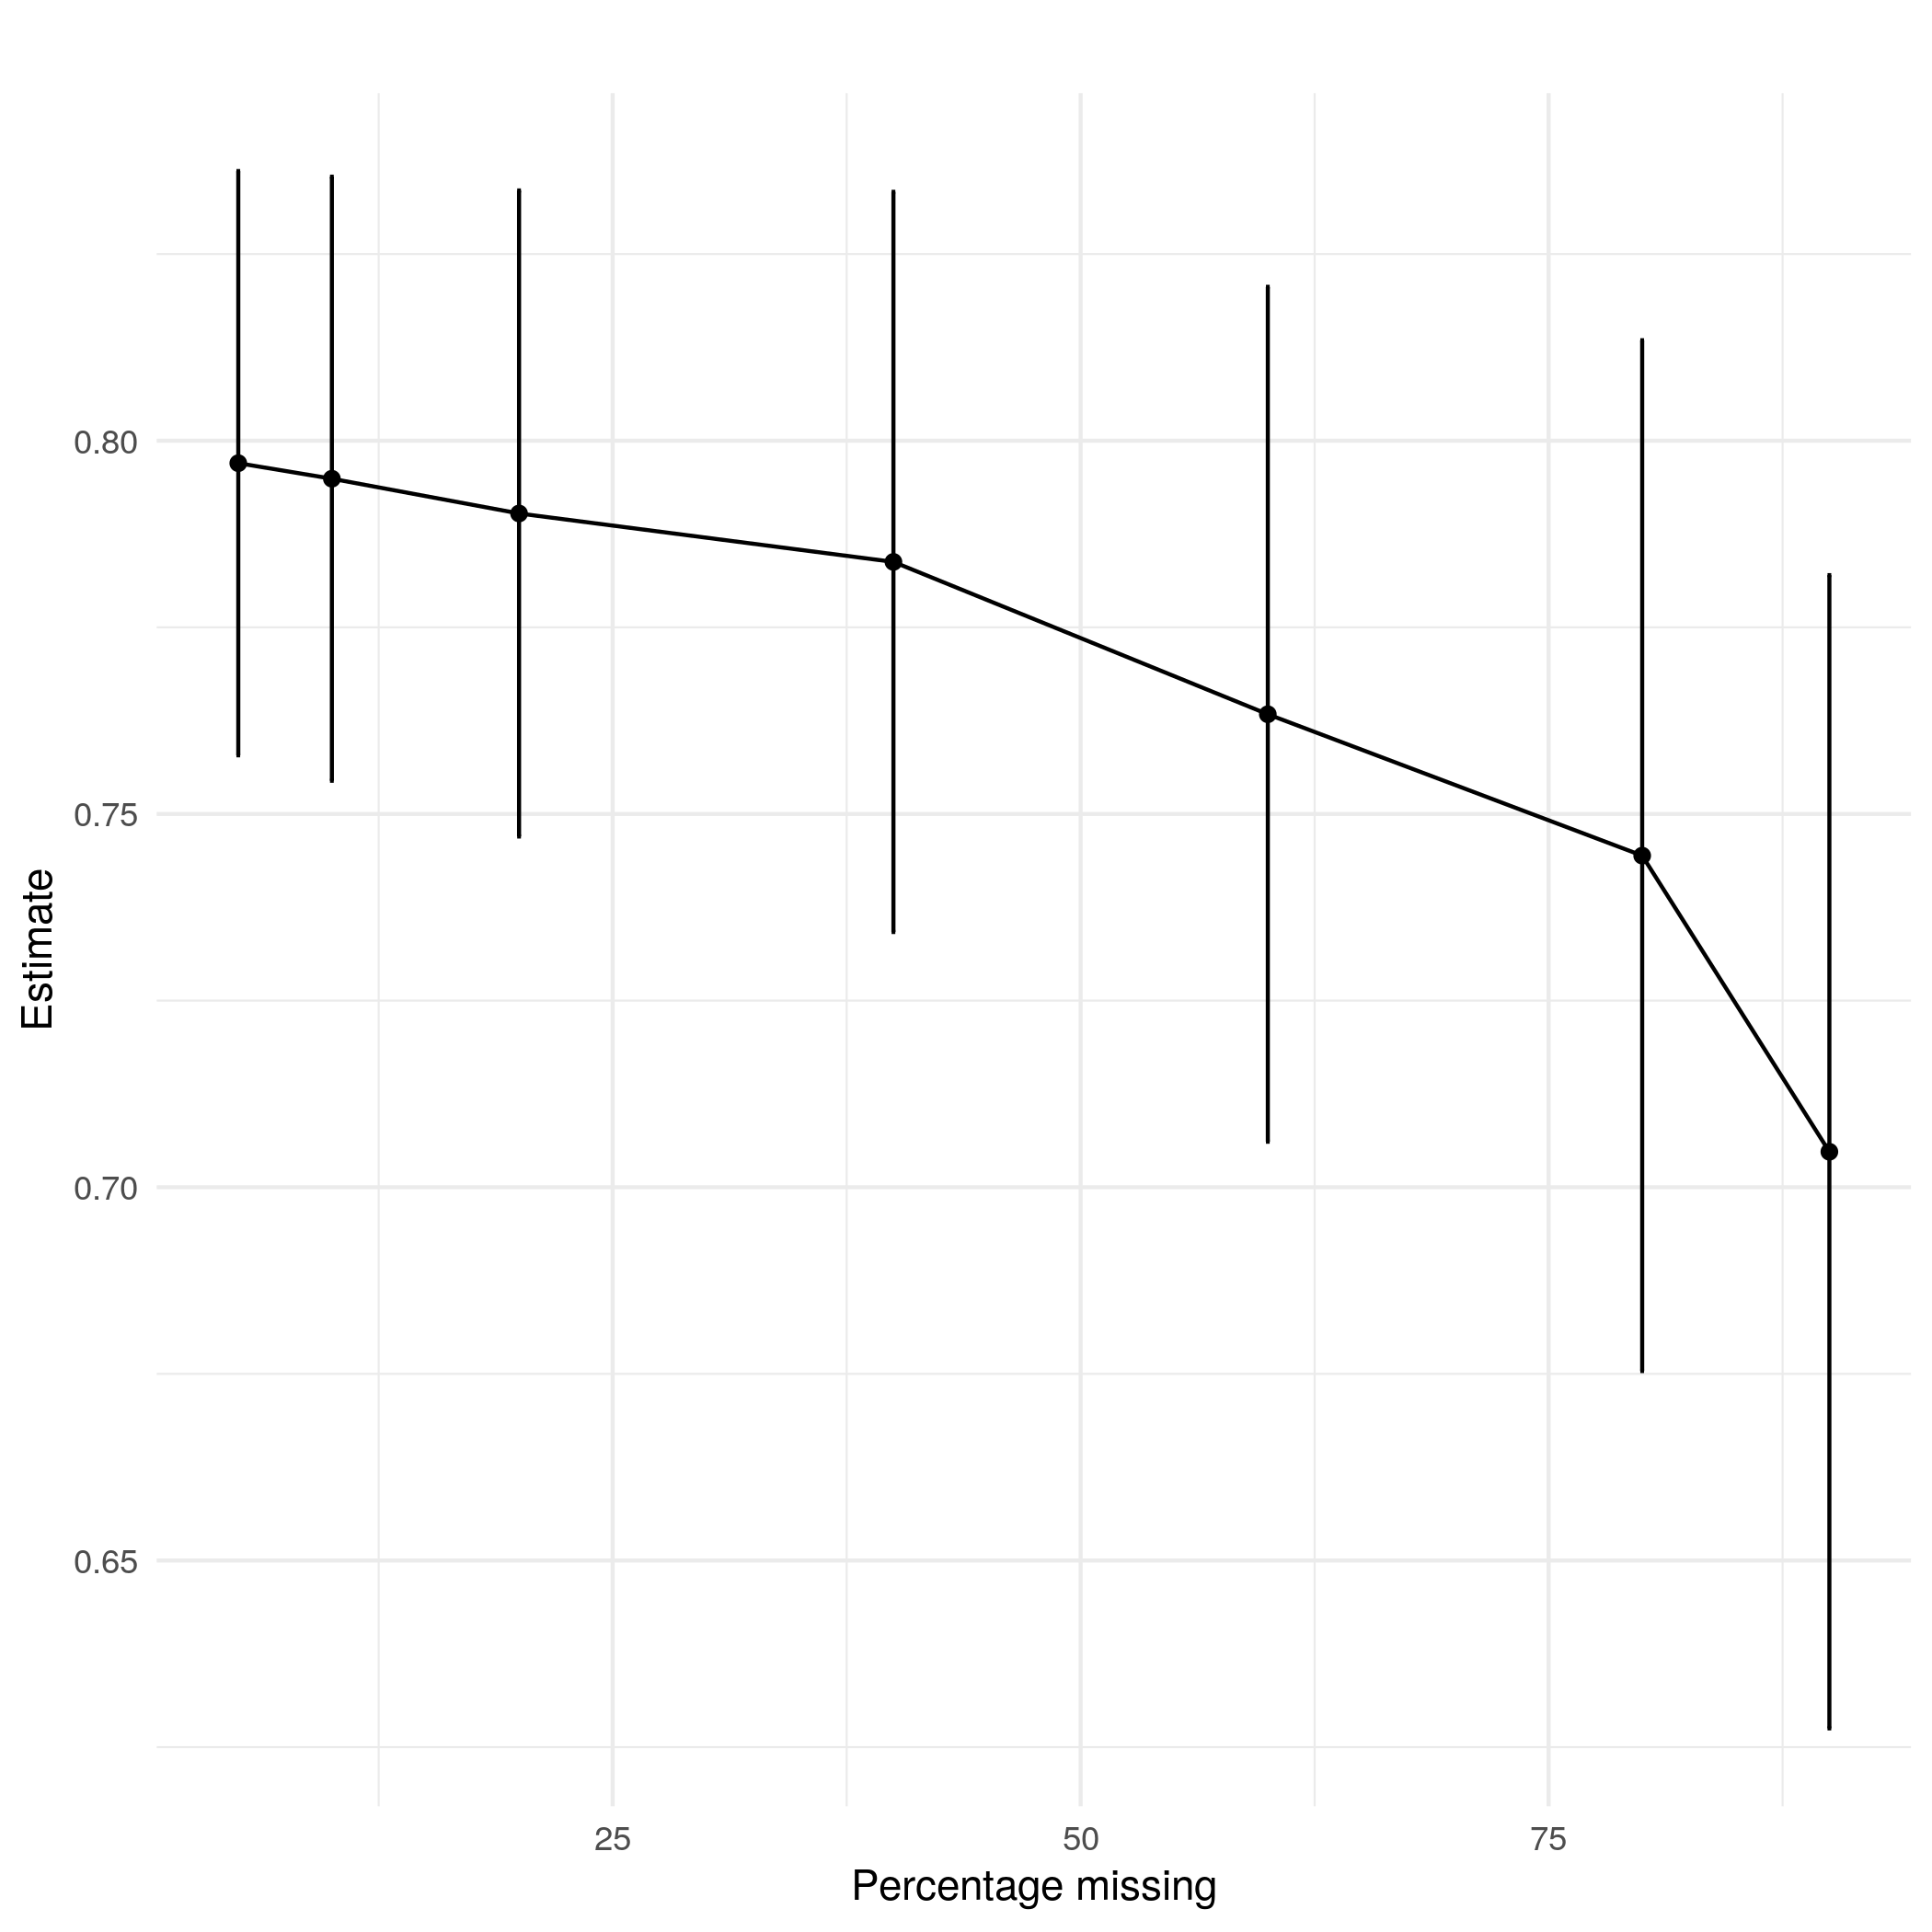
\includegraphics[width=0.4\textwidth]{final_estimate_mi.png}}
		\\
		\subfloat[Coverage]{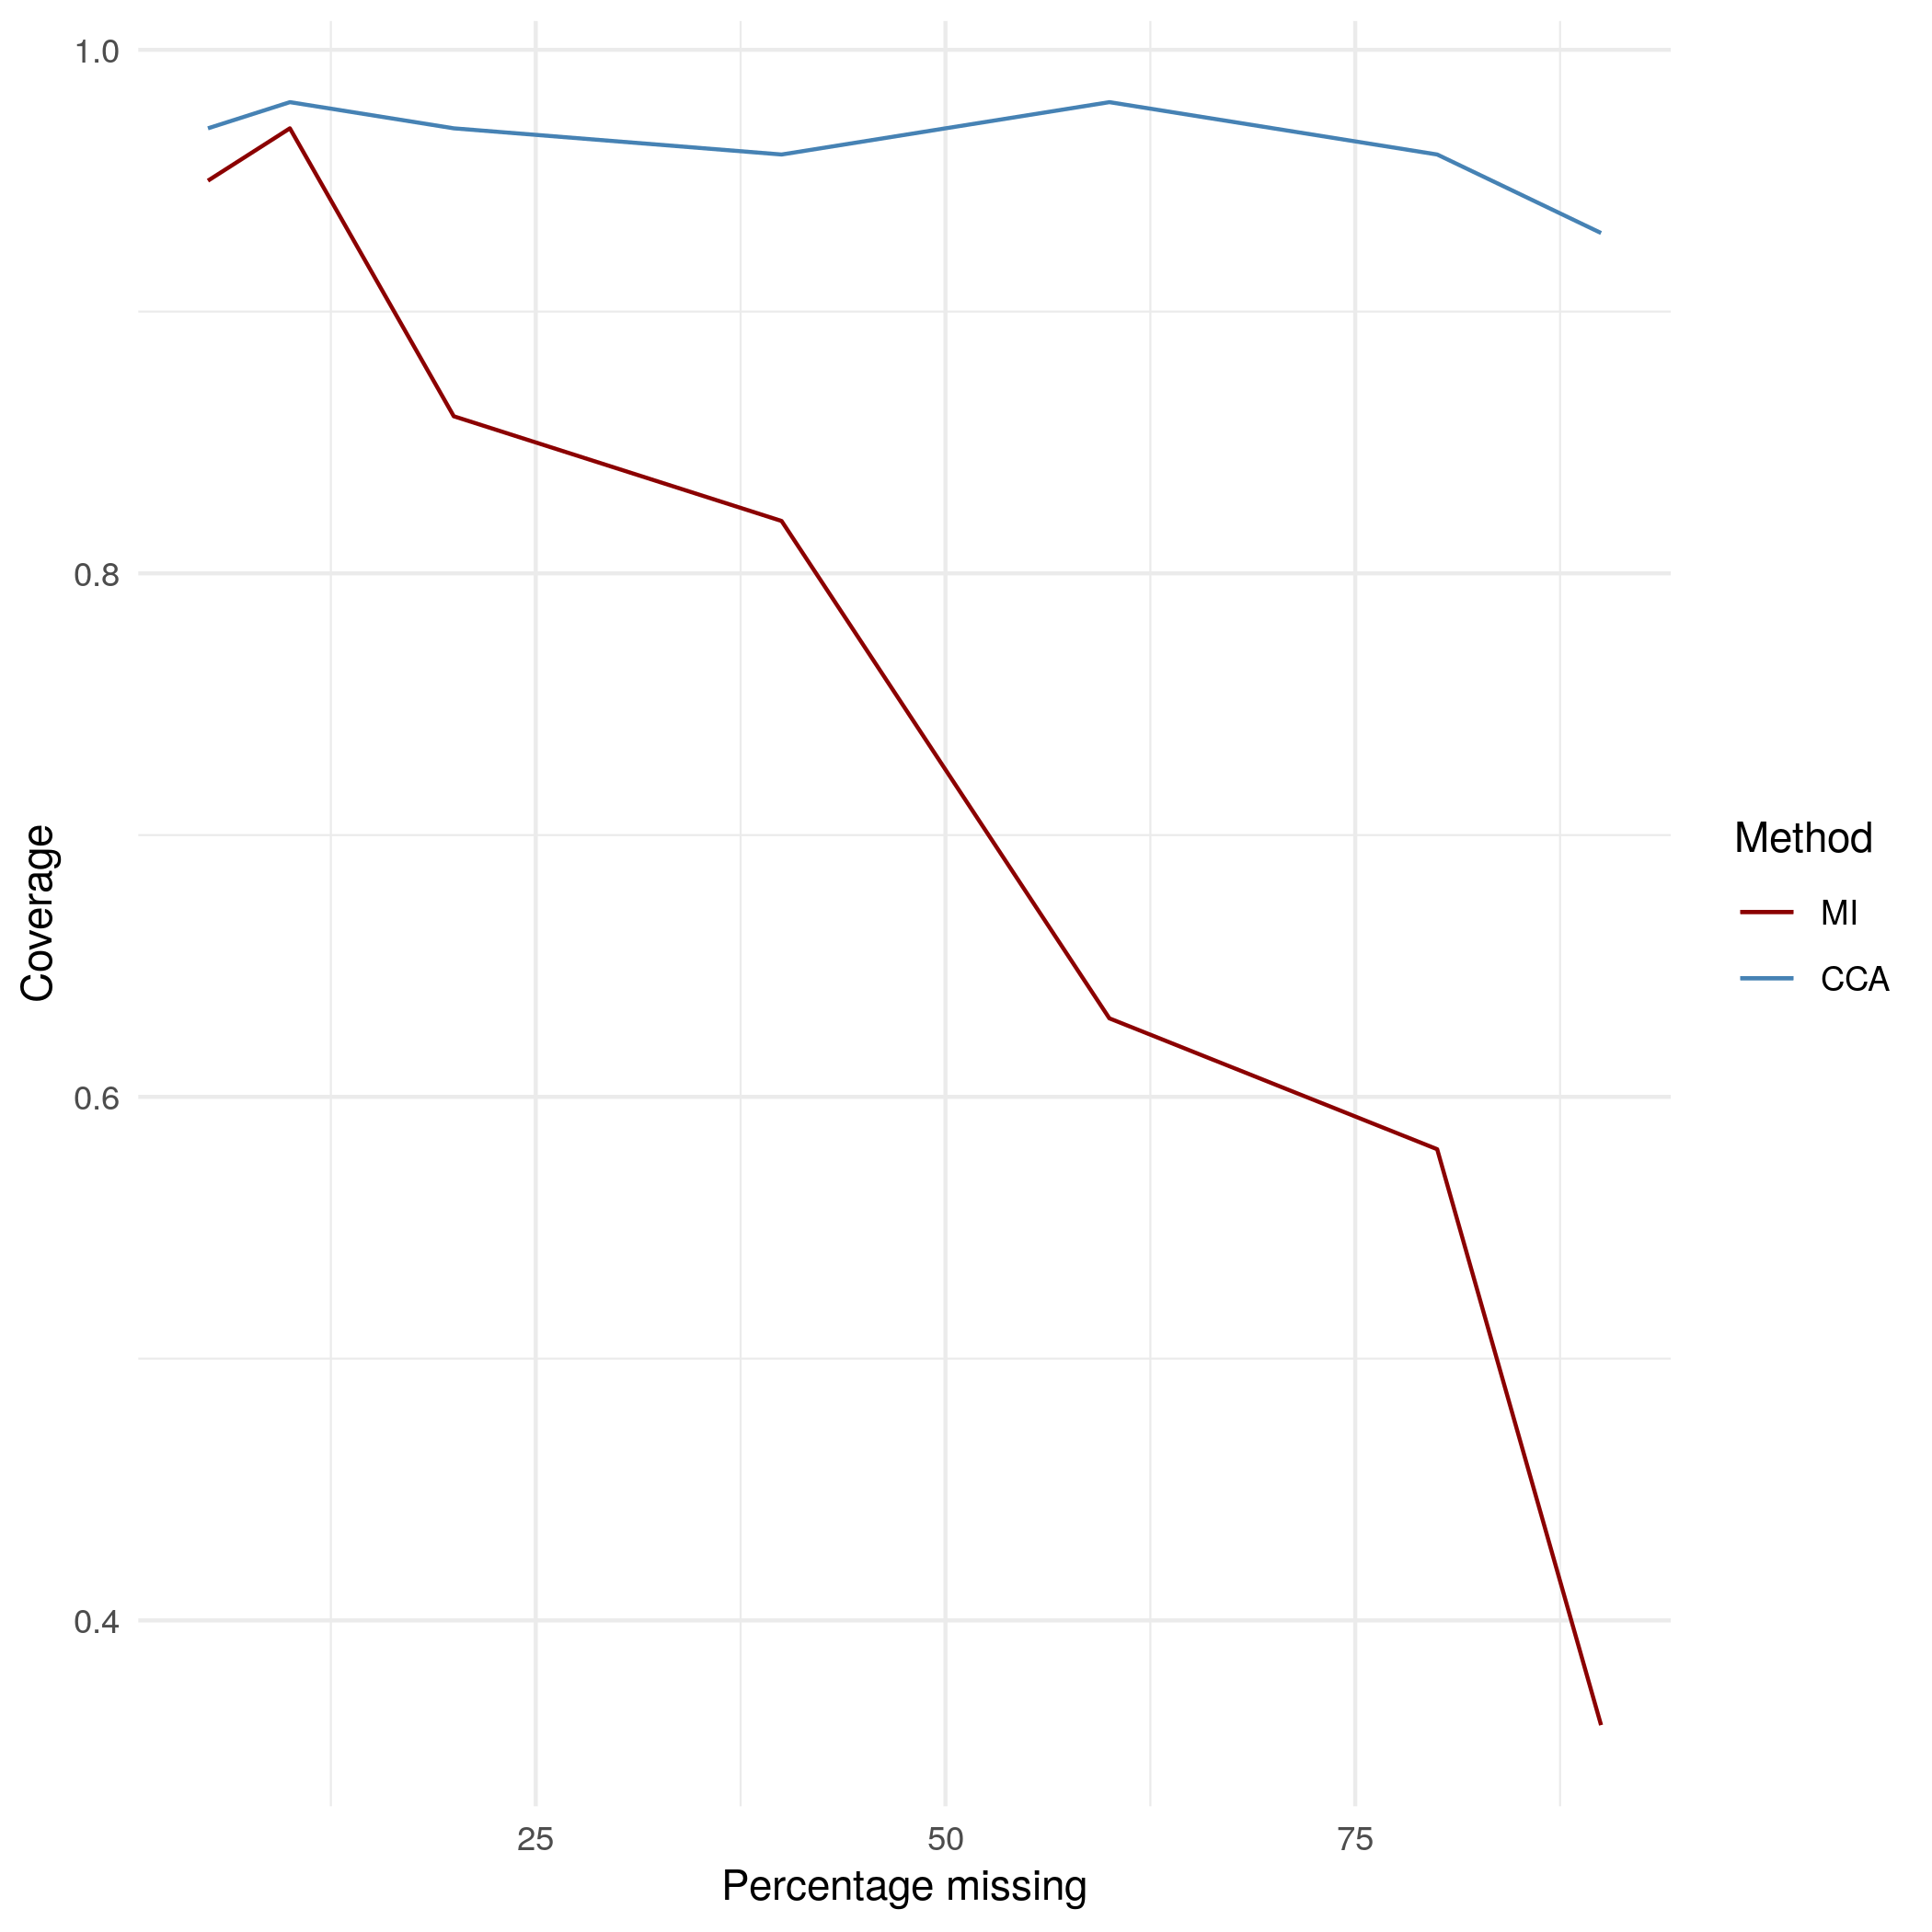
\includegraphics[width=0.3\textwidth]{final_coverage.png}}
		\quad
		\subfloat[Average CI size]{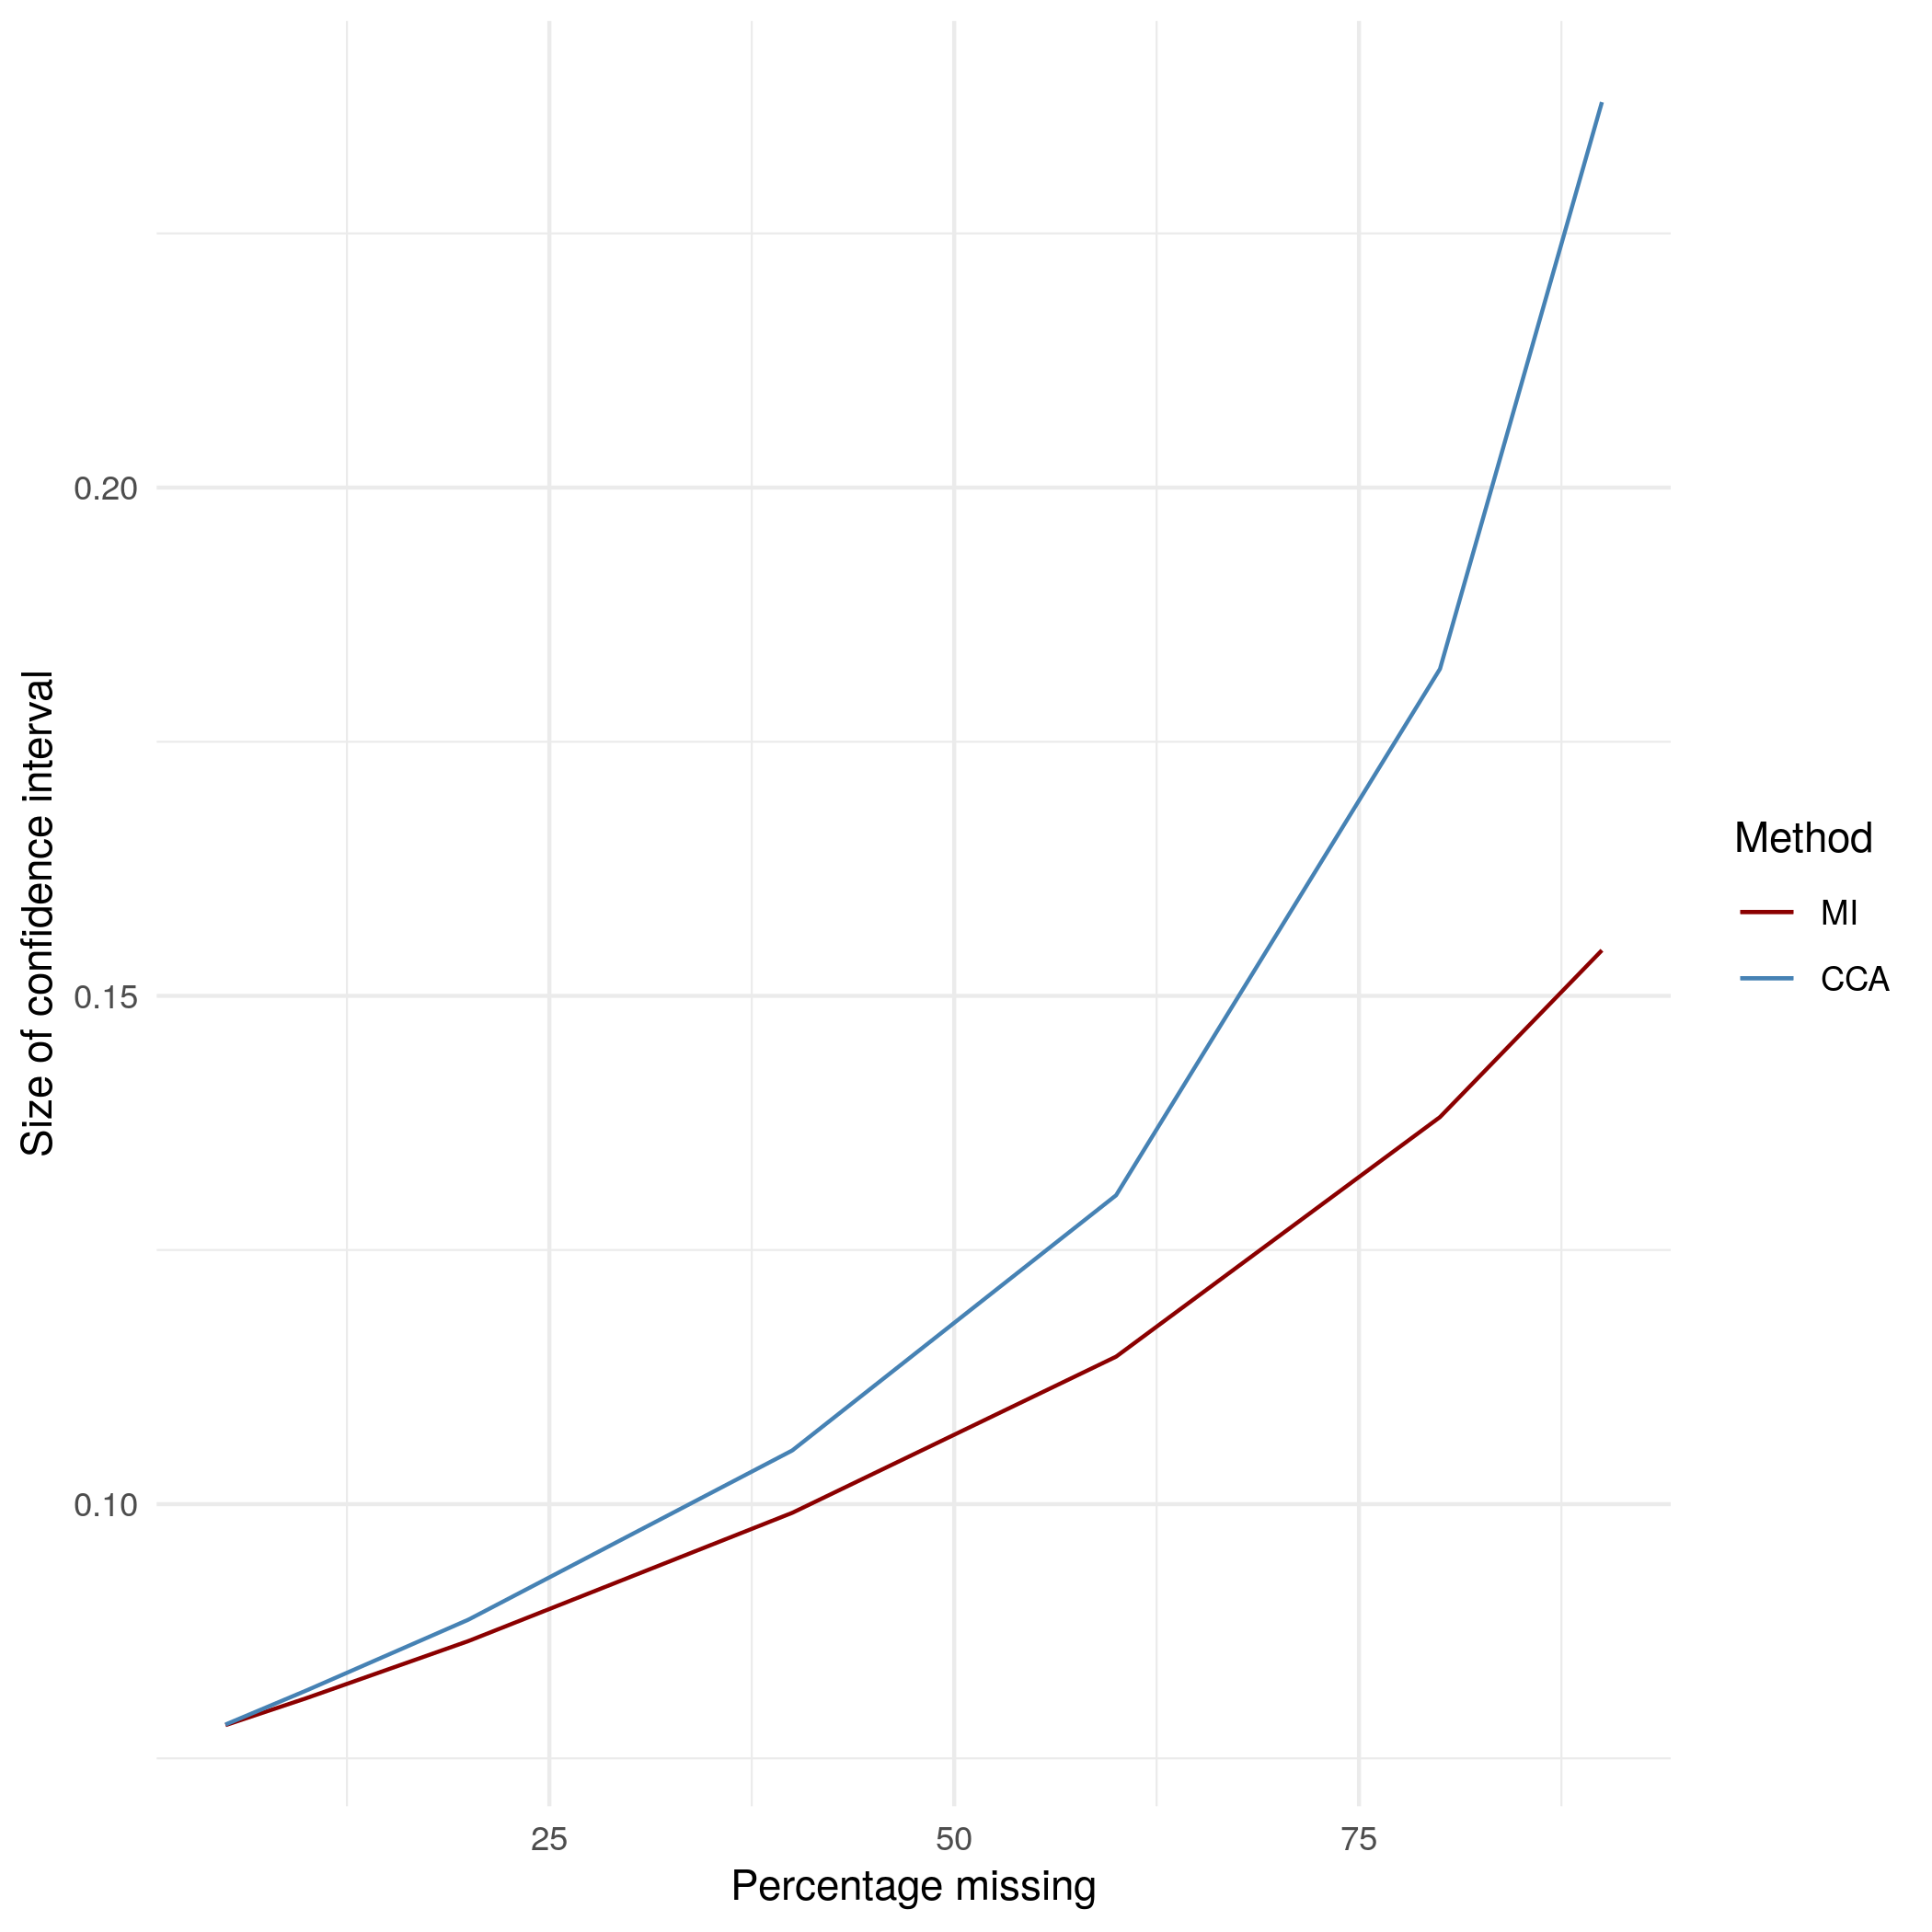
\includegraphics[width=0.3\textwidth]{final_ci.png}}
		\quad
		\subfloat[Average bias]{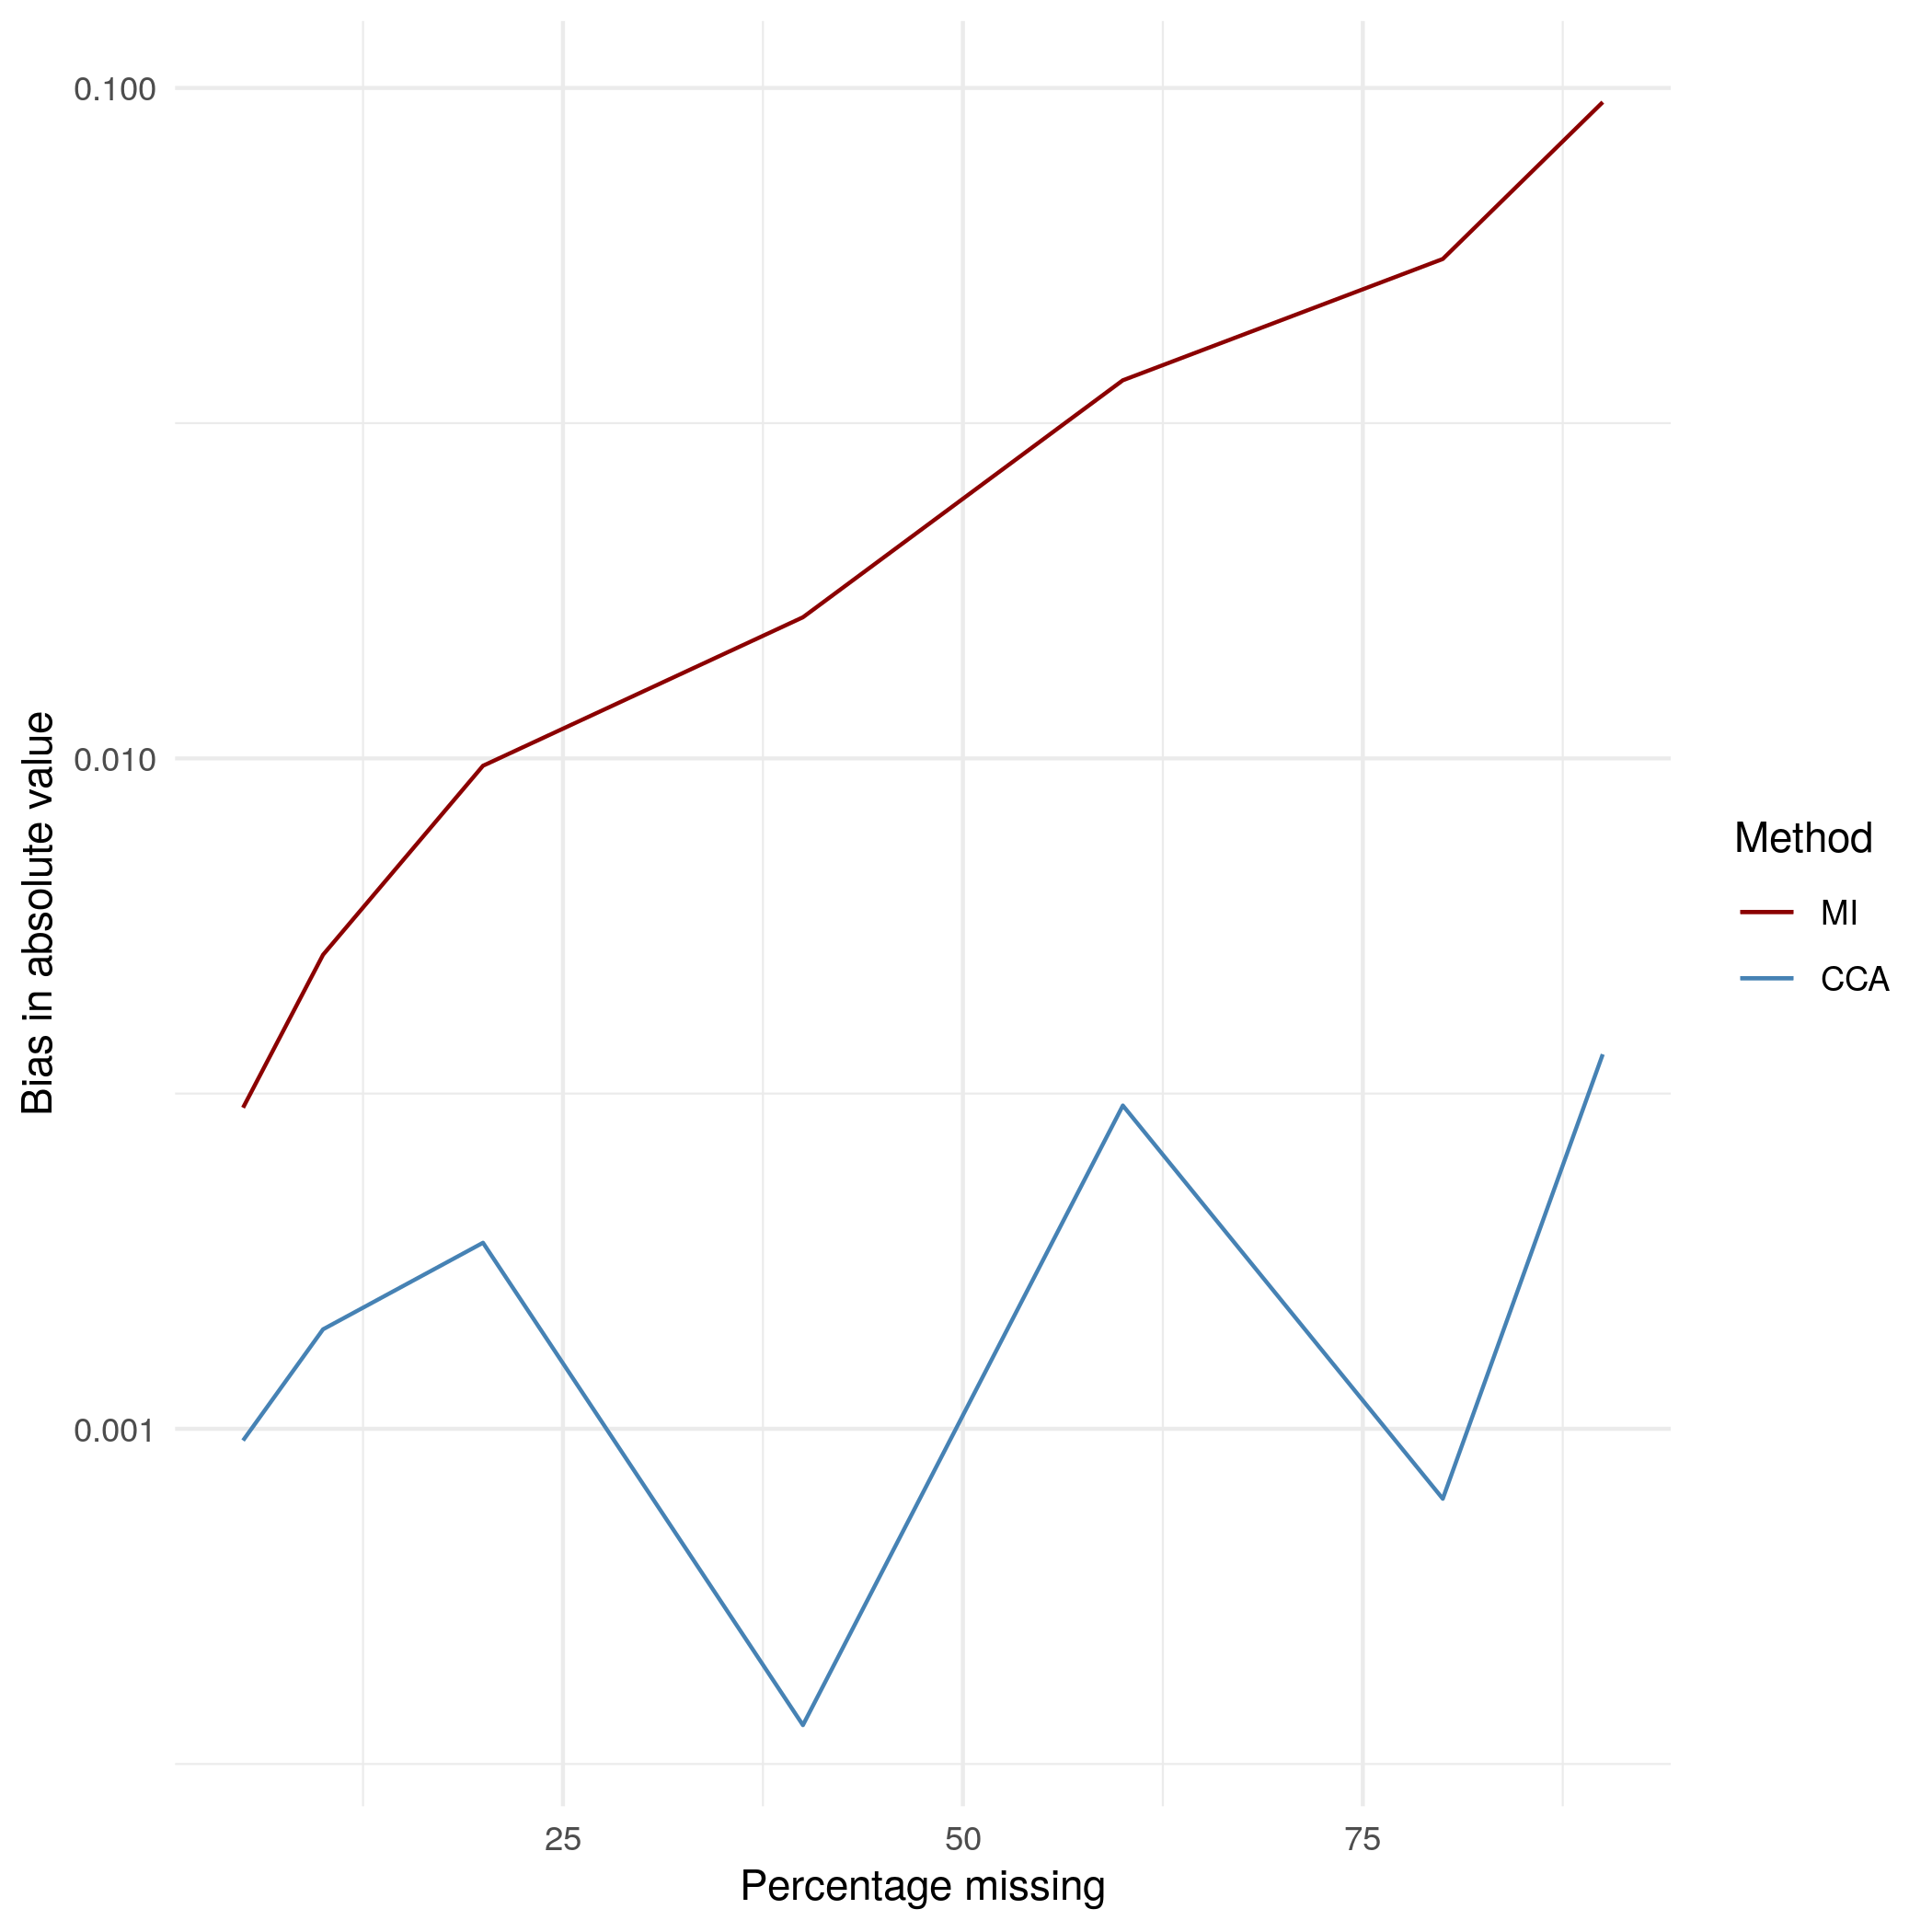
\includegraphics[width=0.3\textwidth]{final_bias.png}}
		\caption{Average results for MAR missingness in $Y$ over 1000 repetitions of the analysis procedure described in 6.2.}
	\end{figure}
	
	In contrast to missingness in $X$, we do not find any benefits from using MI when missingness is in $Y$. In fact, we observe that CCA outperforms MI on all of our metrics. The strong performance of CCA on its own is surprising, and suggests that the data is MCAR rather than MAR despite use of the logit function to remove data.
	
	\subsubsection{MNAR}

	\begin{figure}[H]
		\centering
		\subfloat[$\beta_{1}$ estimate with CCA]{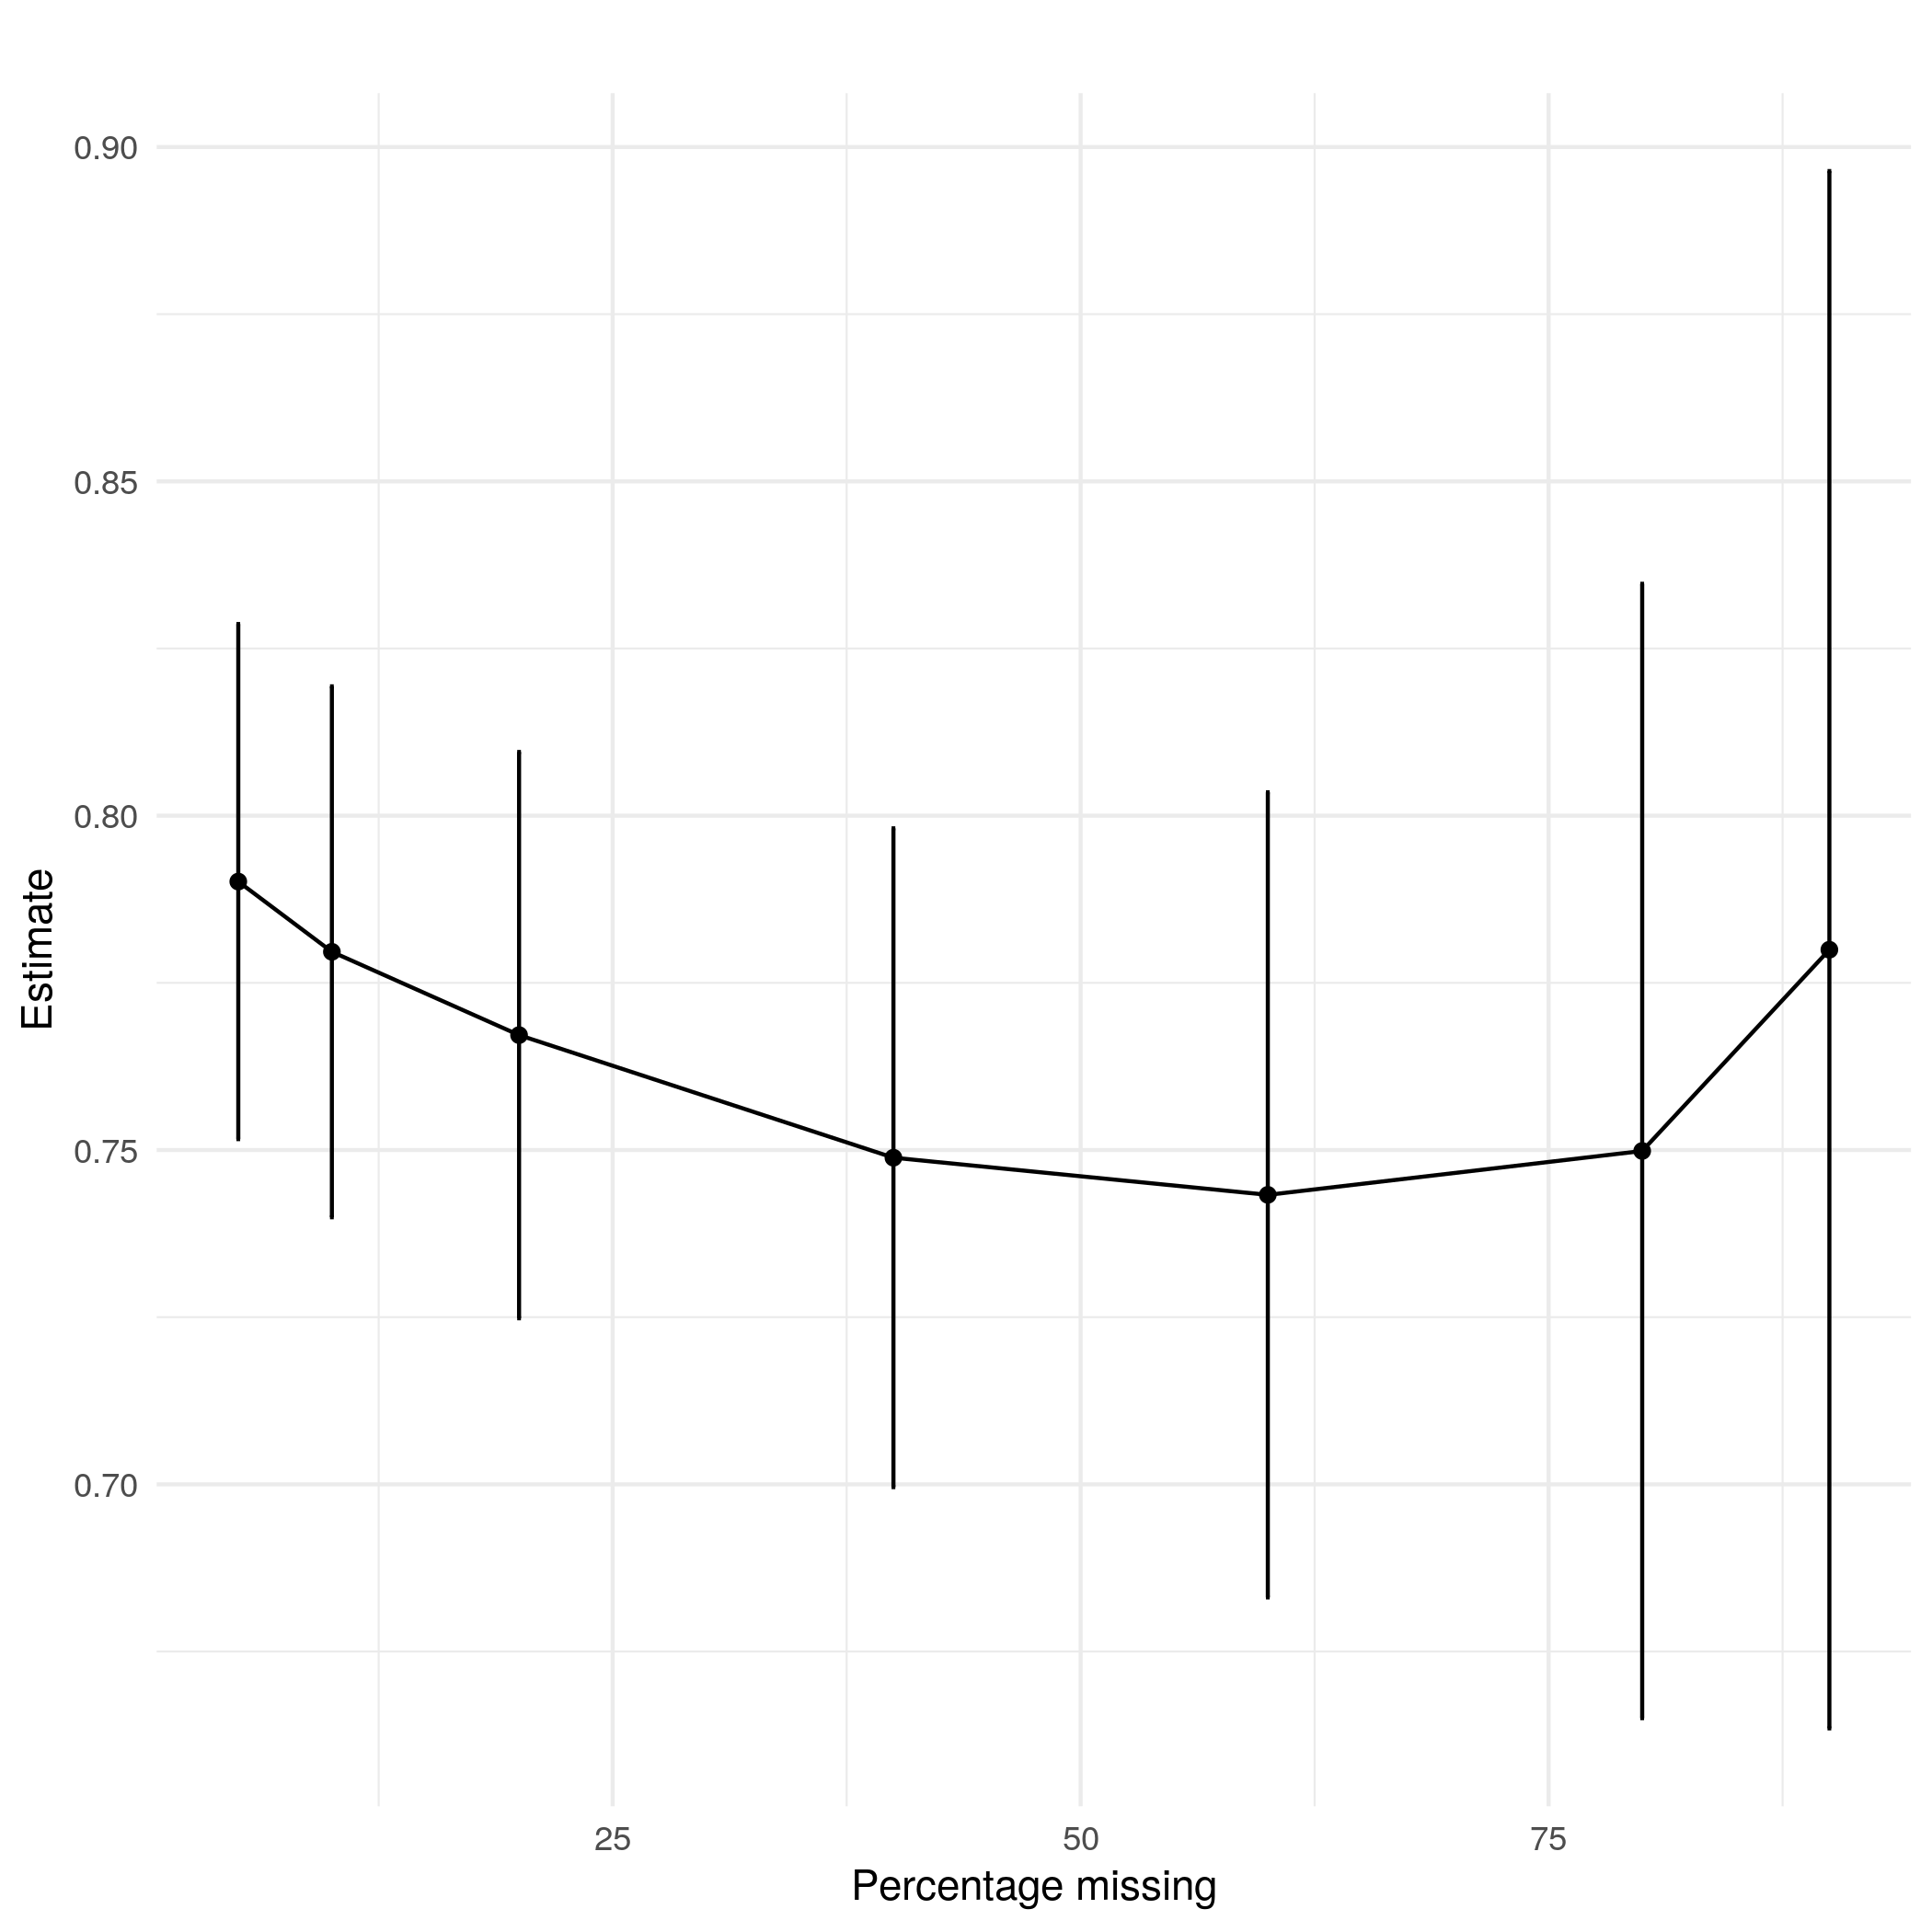
\includegraphics[width=0.4\textwidth]{mnar_final_estimate_cca.png}}
		\quad
		\subfloat[$\beta_{1}$ estimate with MI]{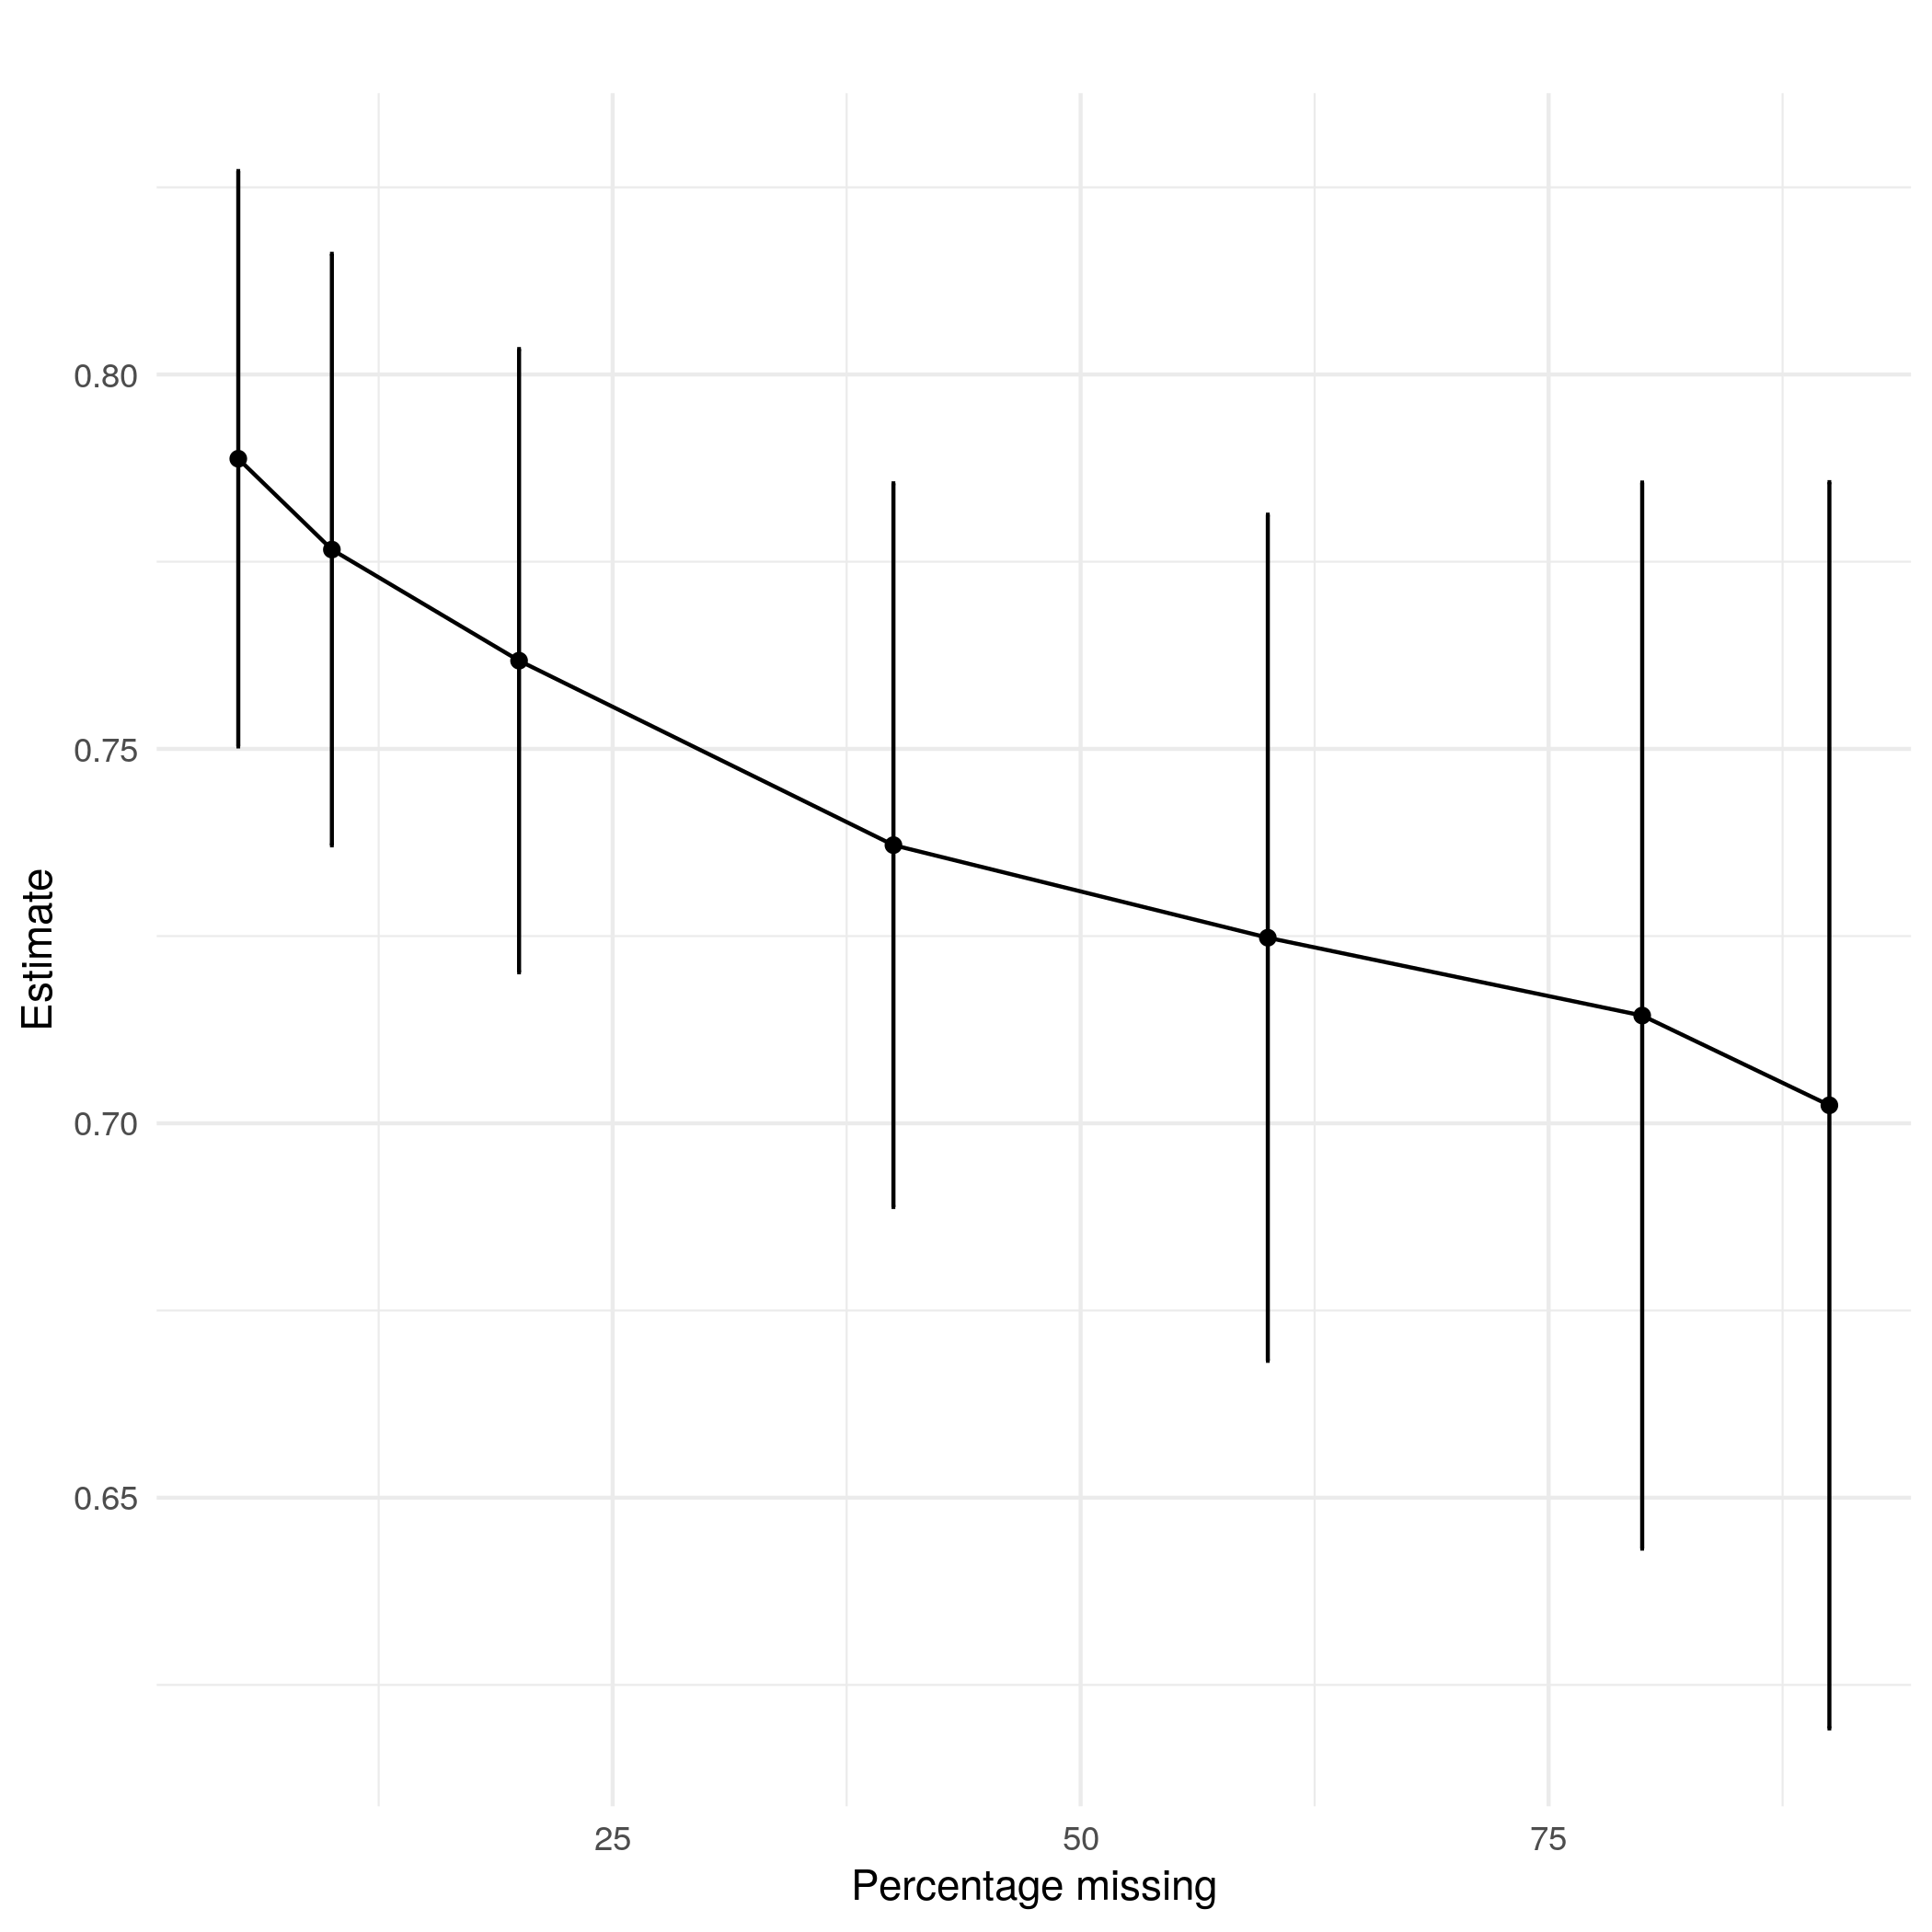
\includegraphics[width=0.4\textwidth]{mnar_final_estimate_mi.png}}
		\\
		\subfloat[Coverage]{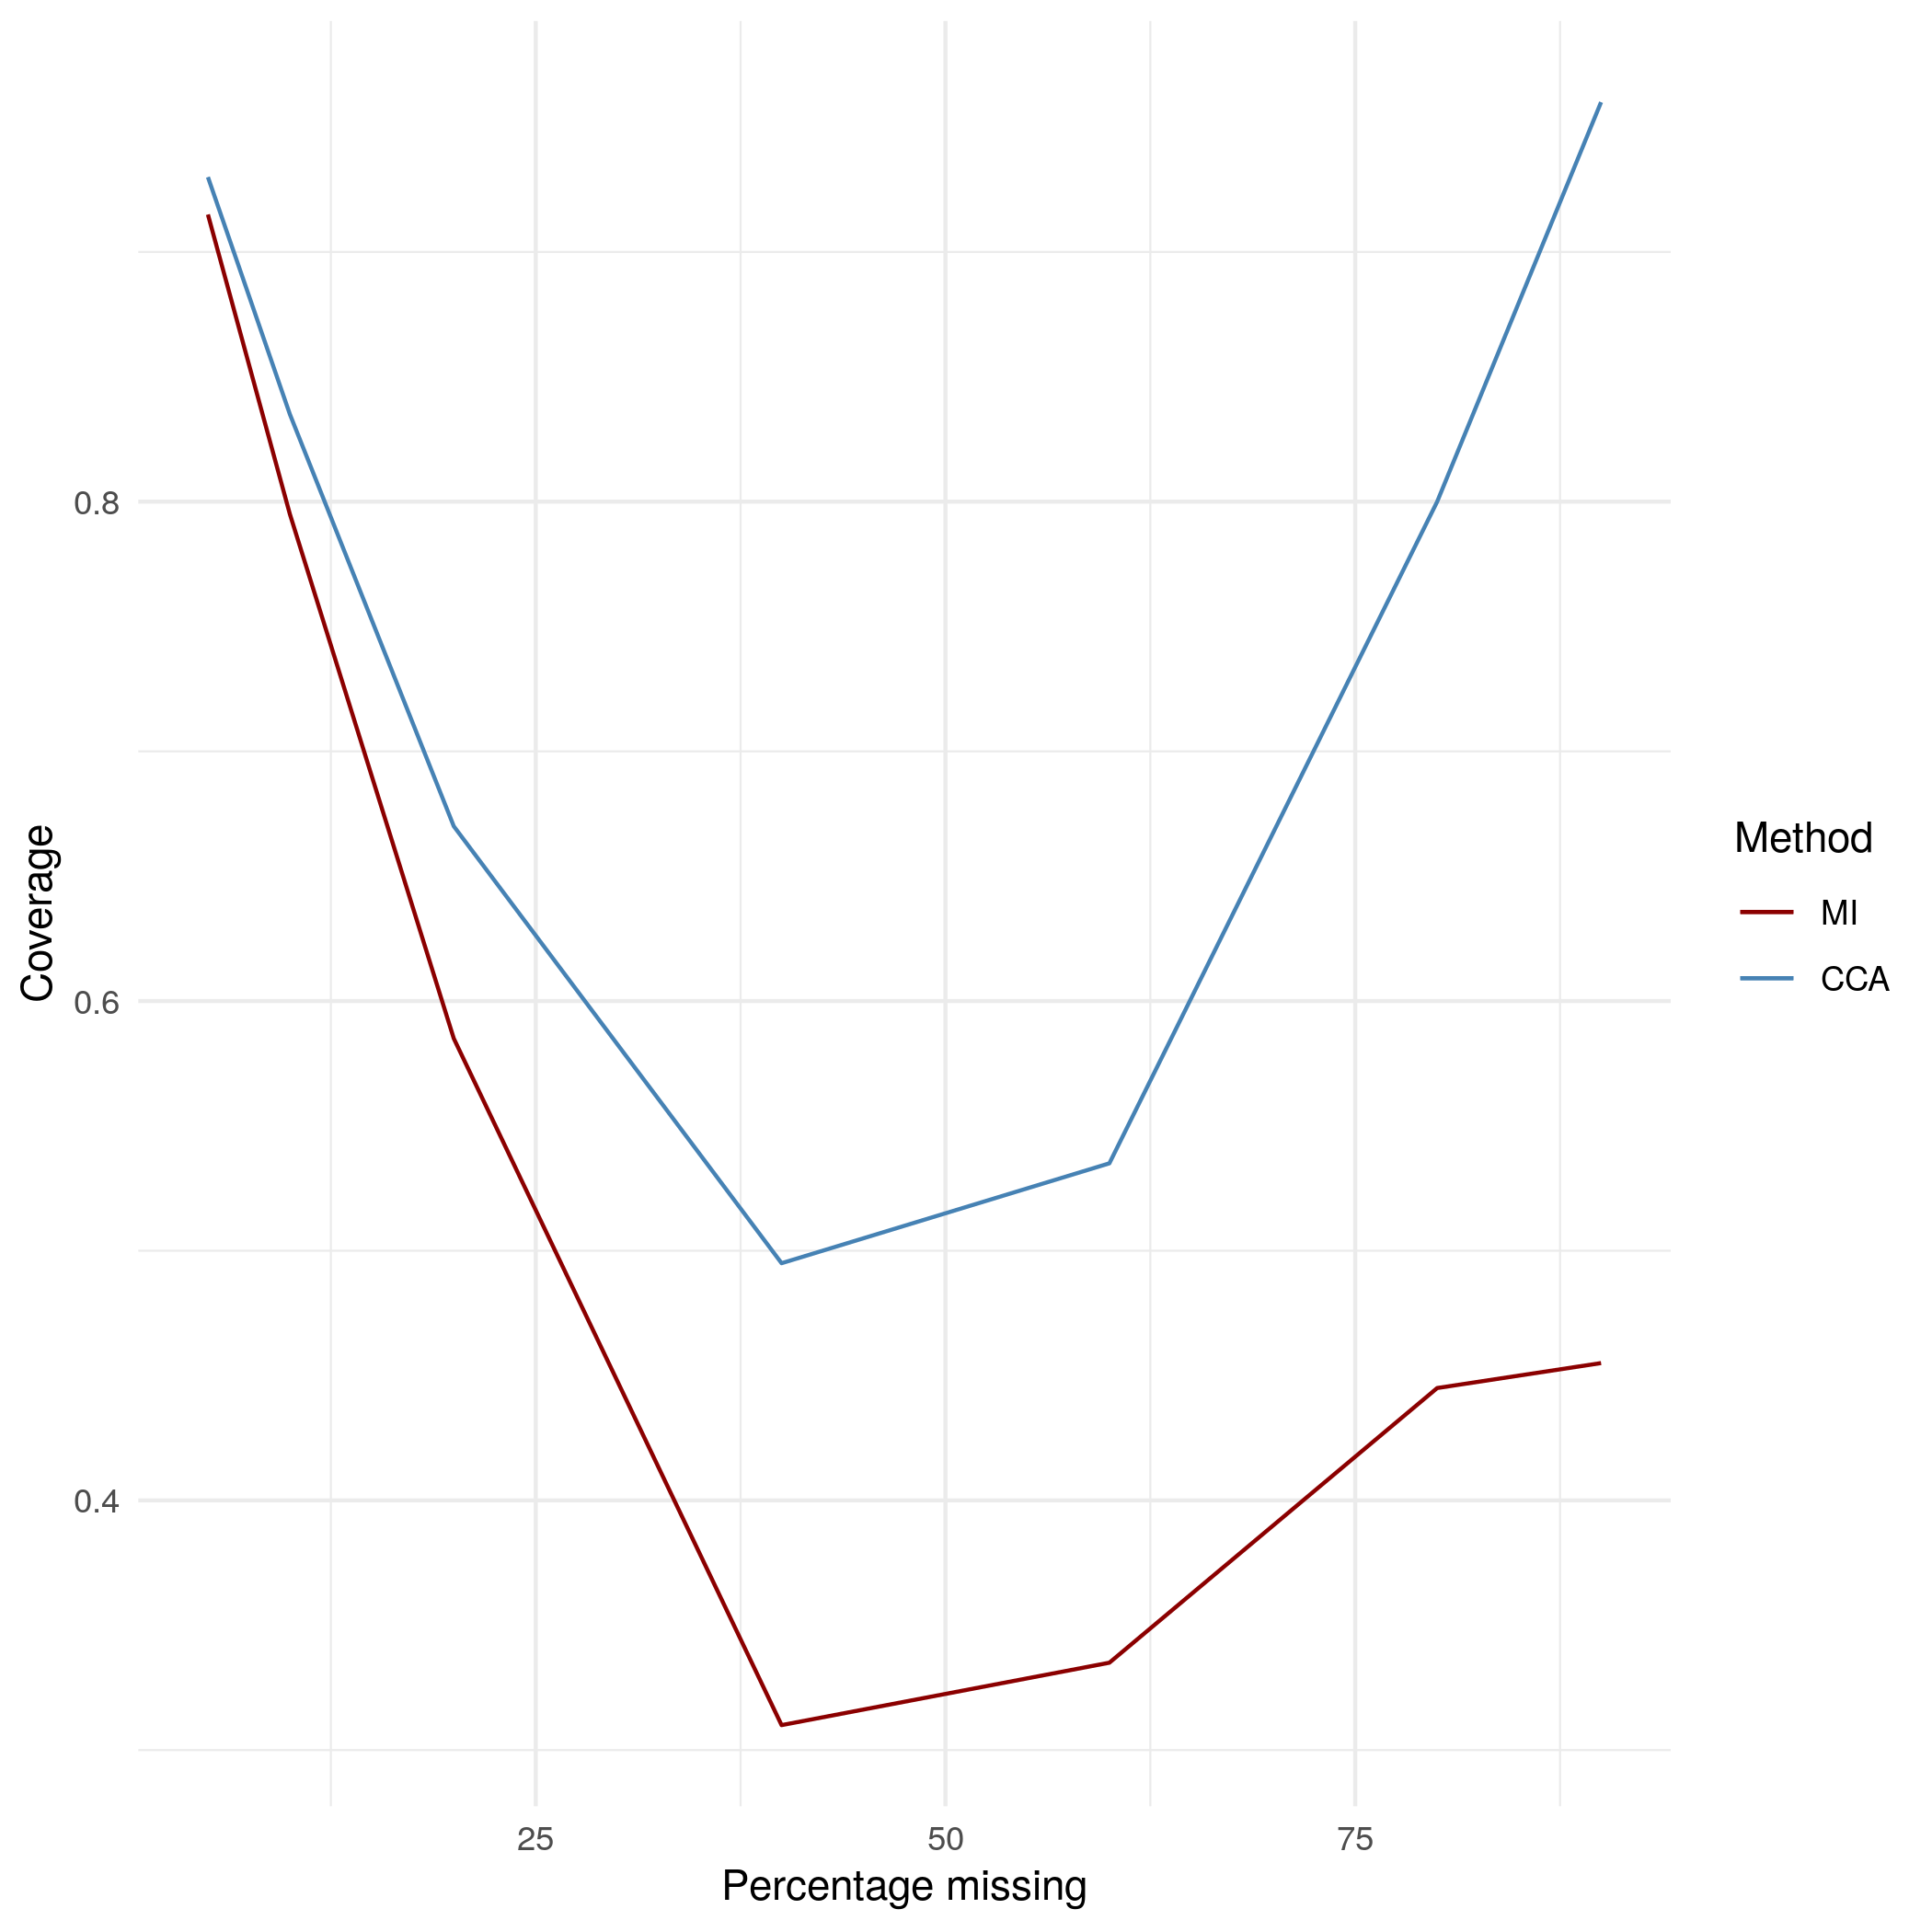
\includegraphics[width=0.3\textwidth]{mnar_final_coverage.png}}
		\quad
		\subfloat[Average CI size]{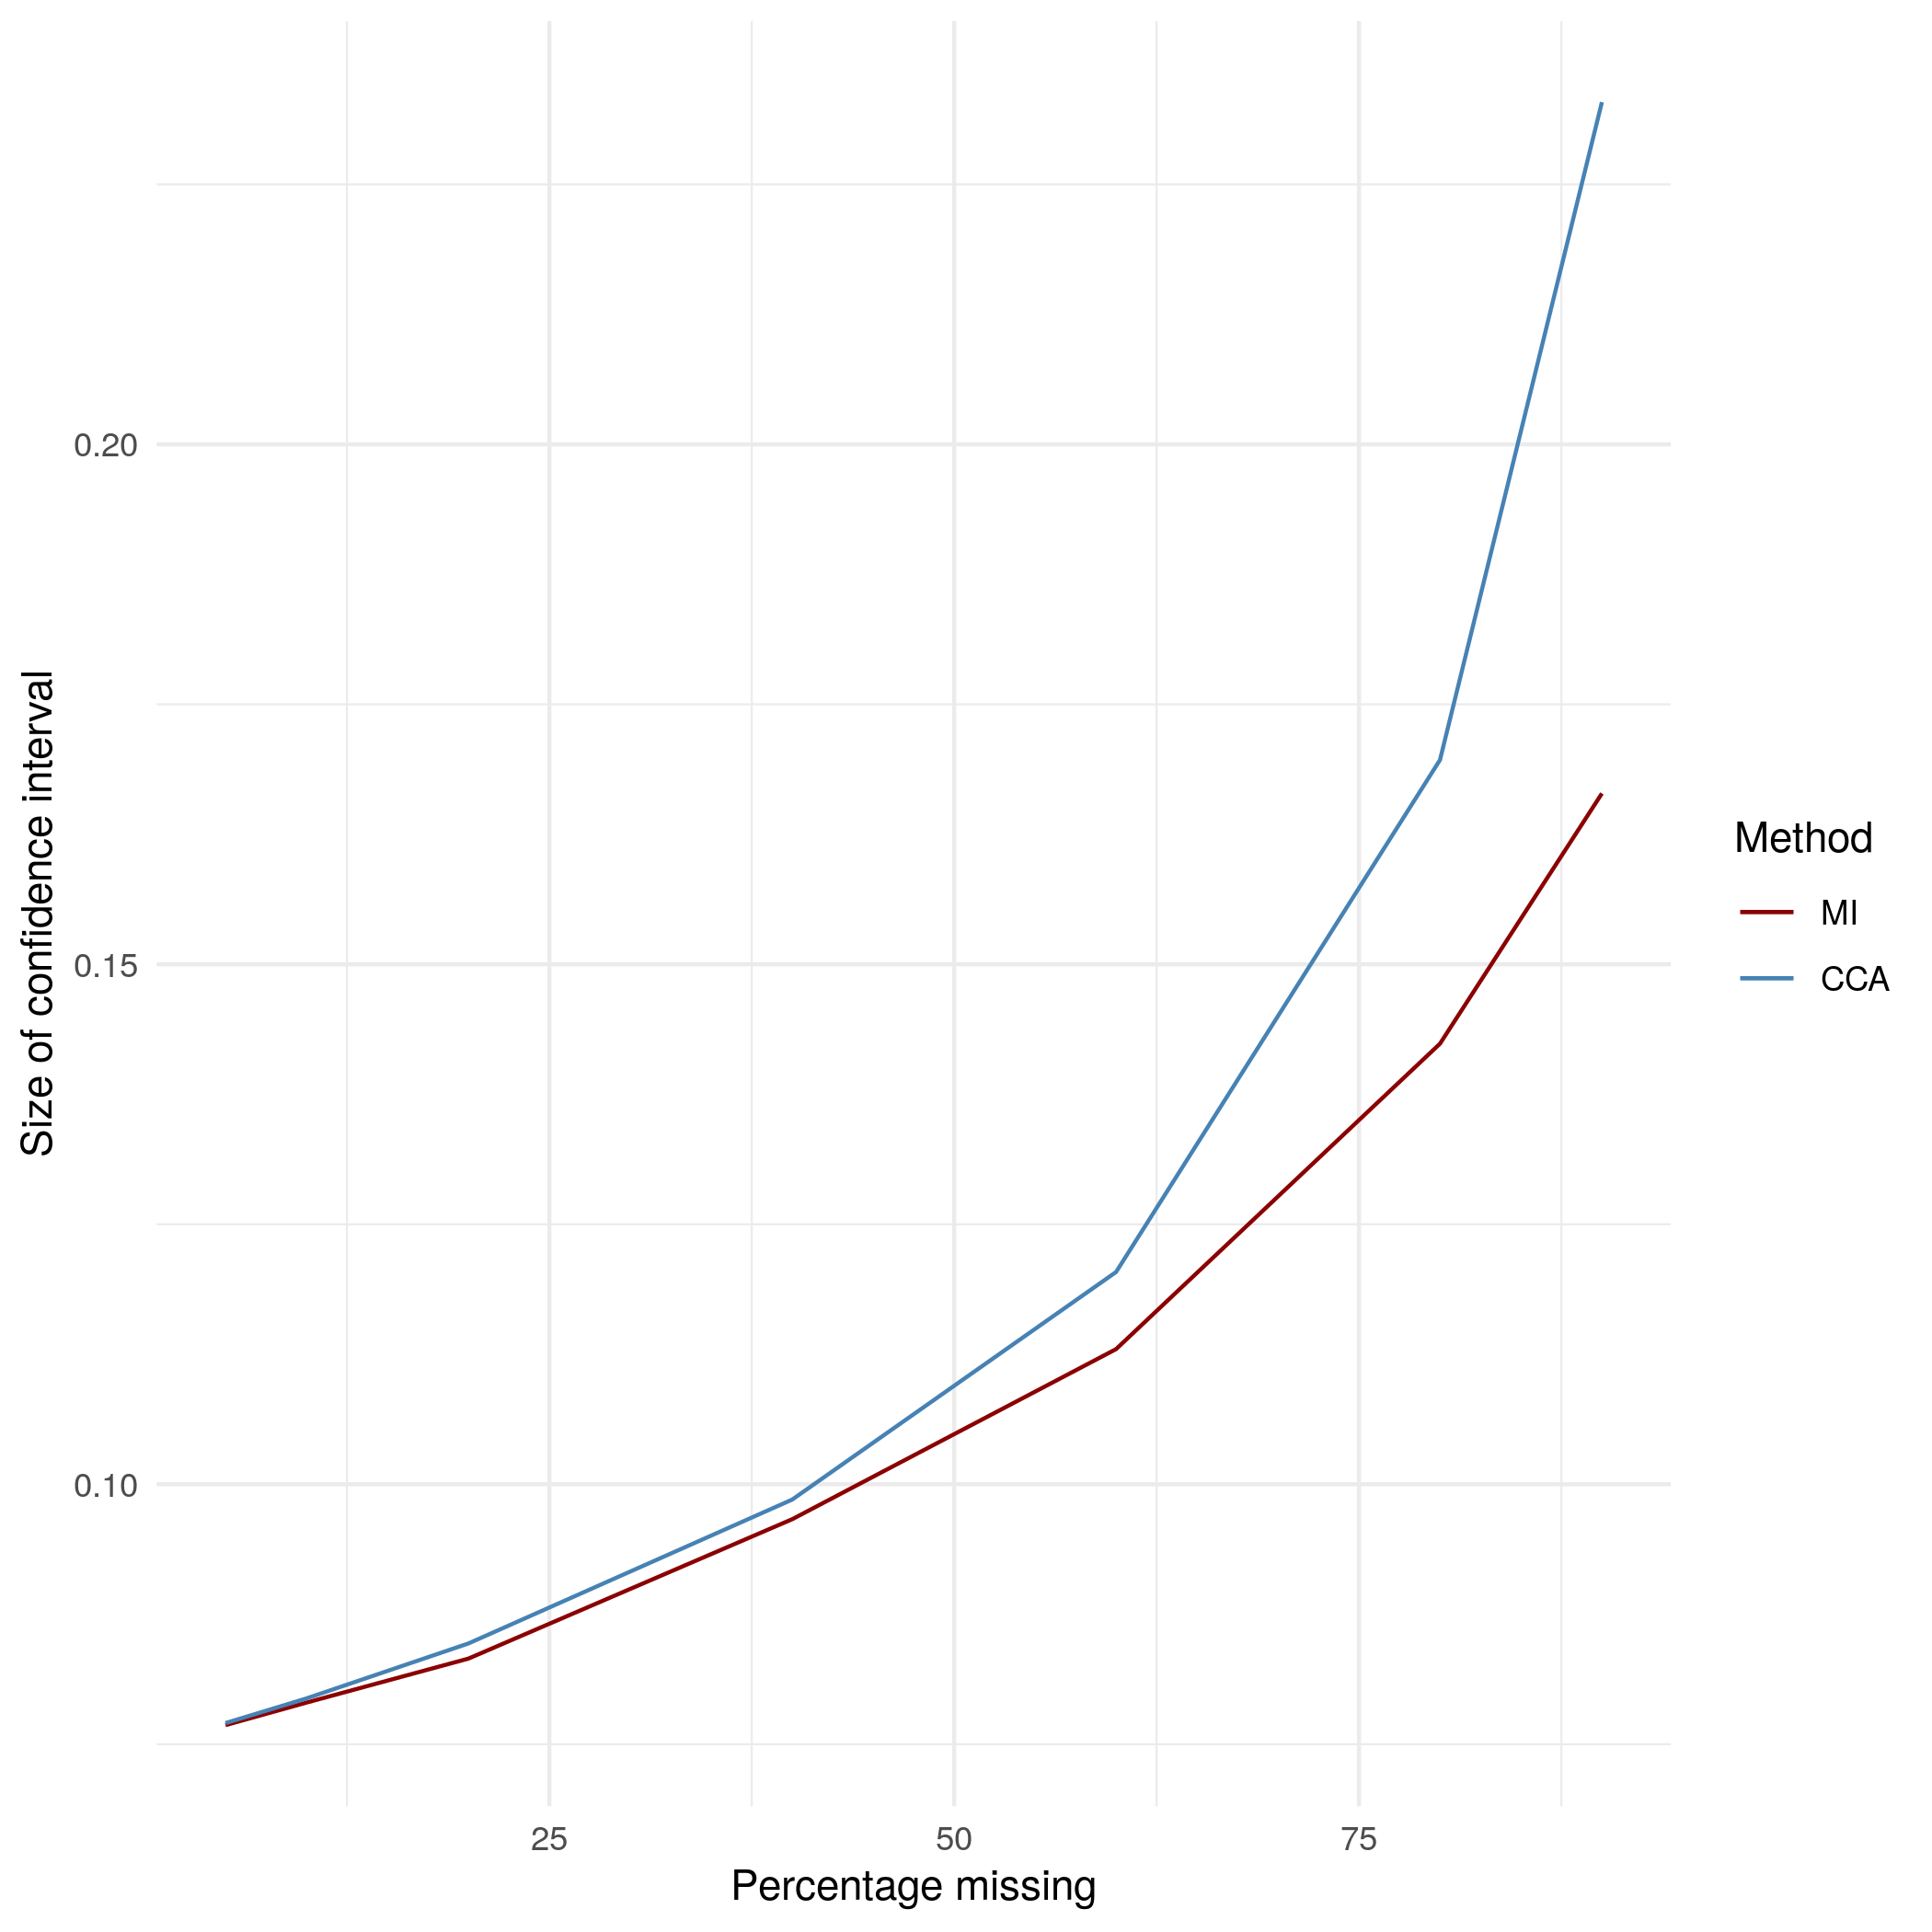
\includegraphics[width=0.3\textwidth]{mnar_final_ci.png}}
		\quad
		\subfloat[Average bias]{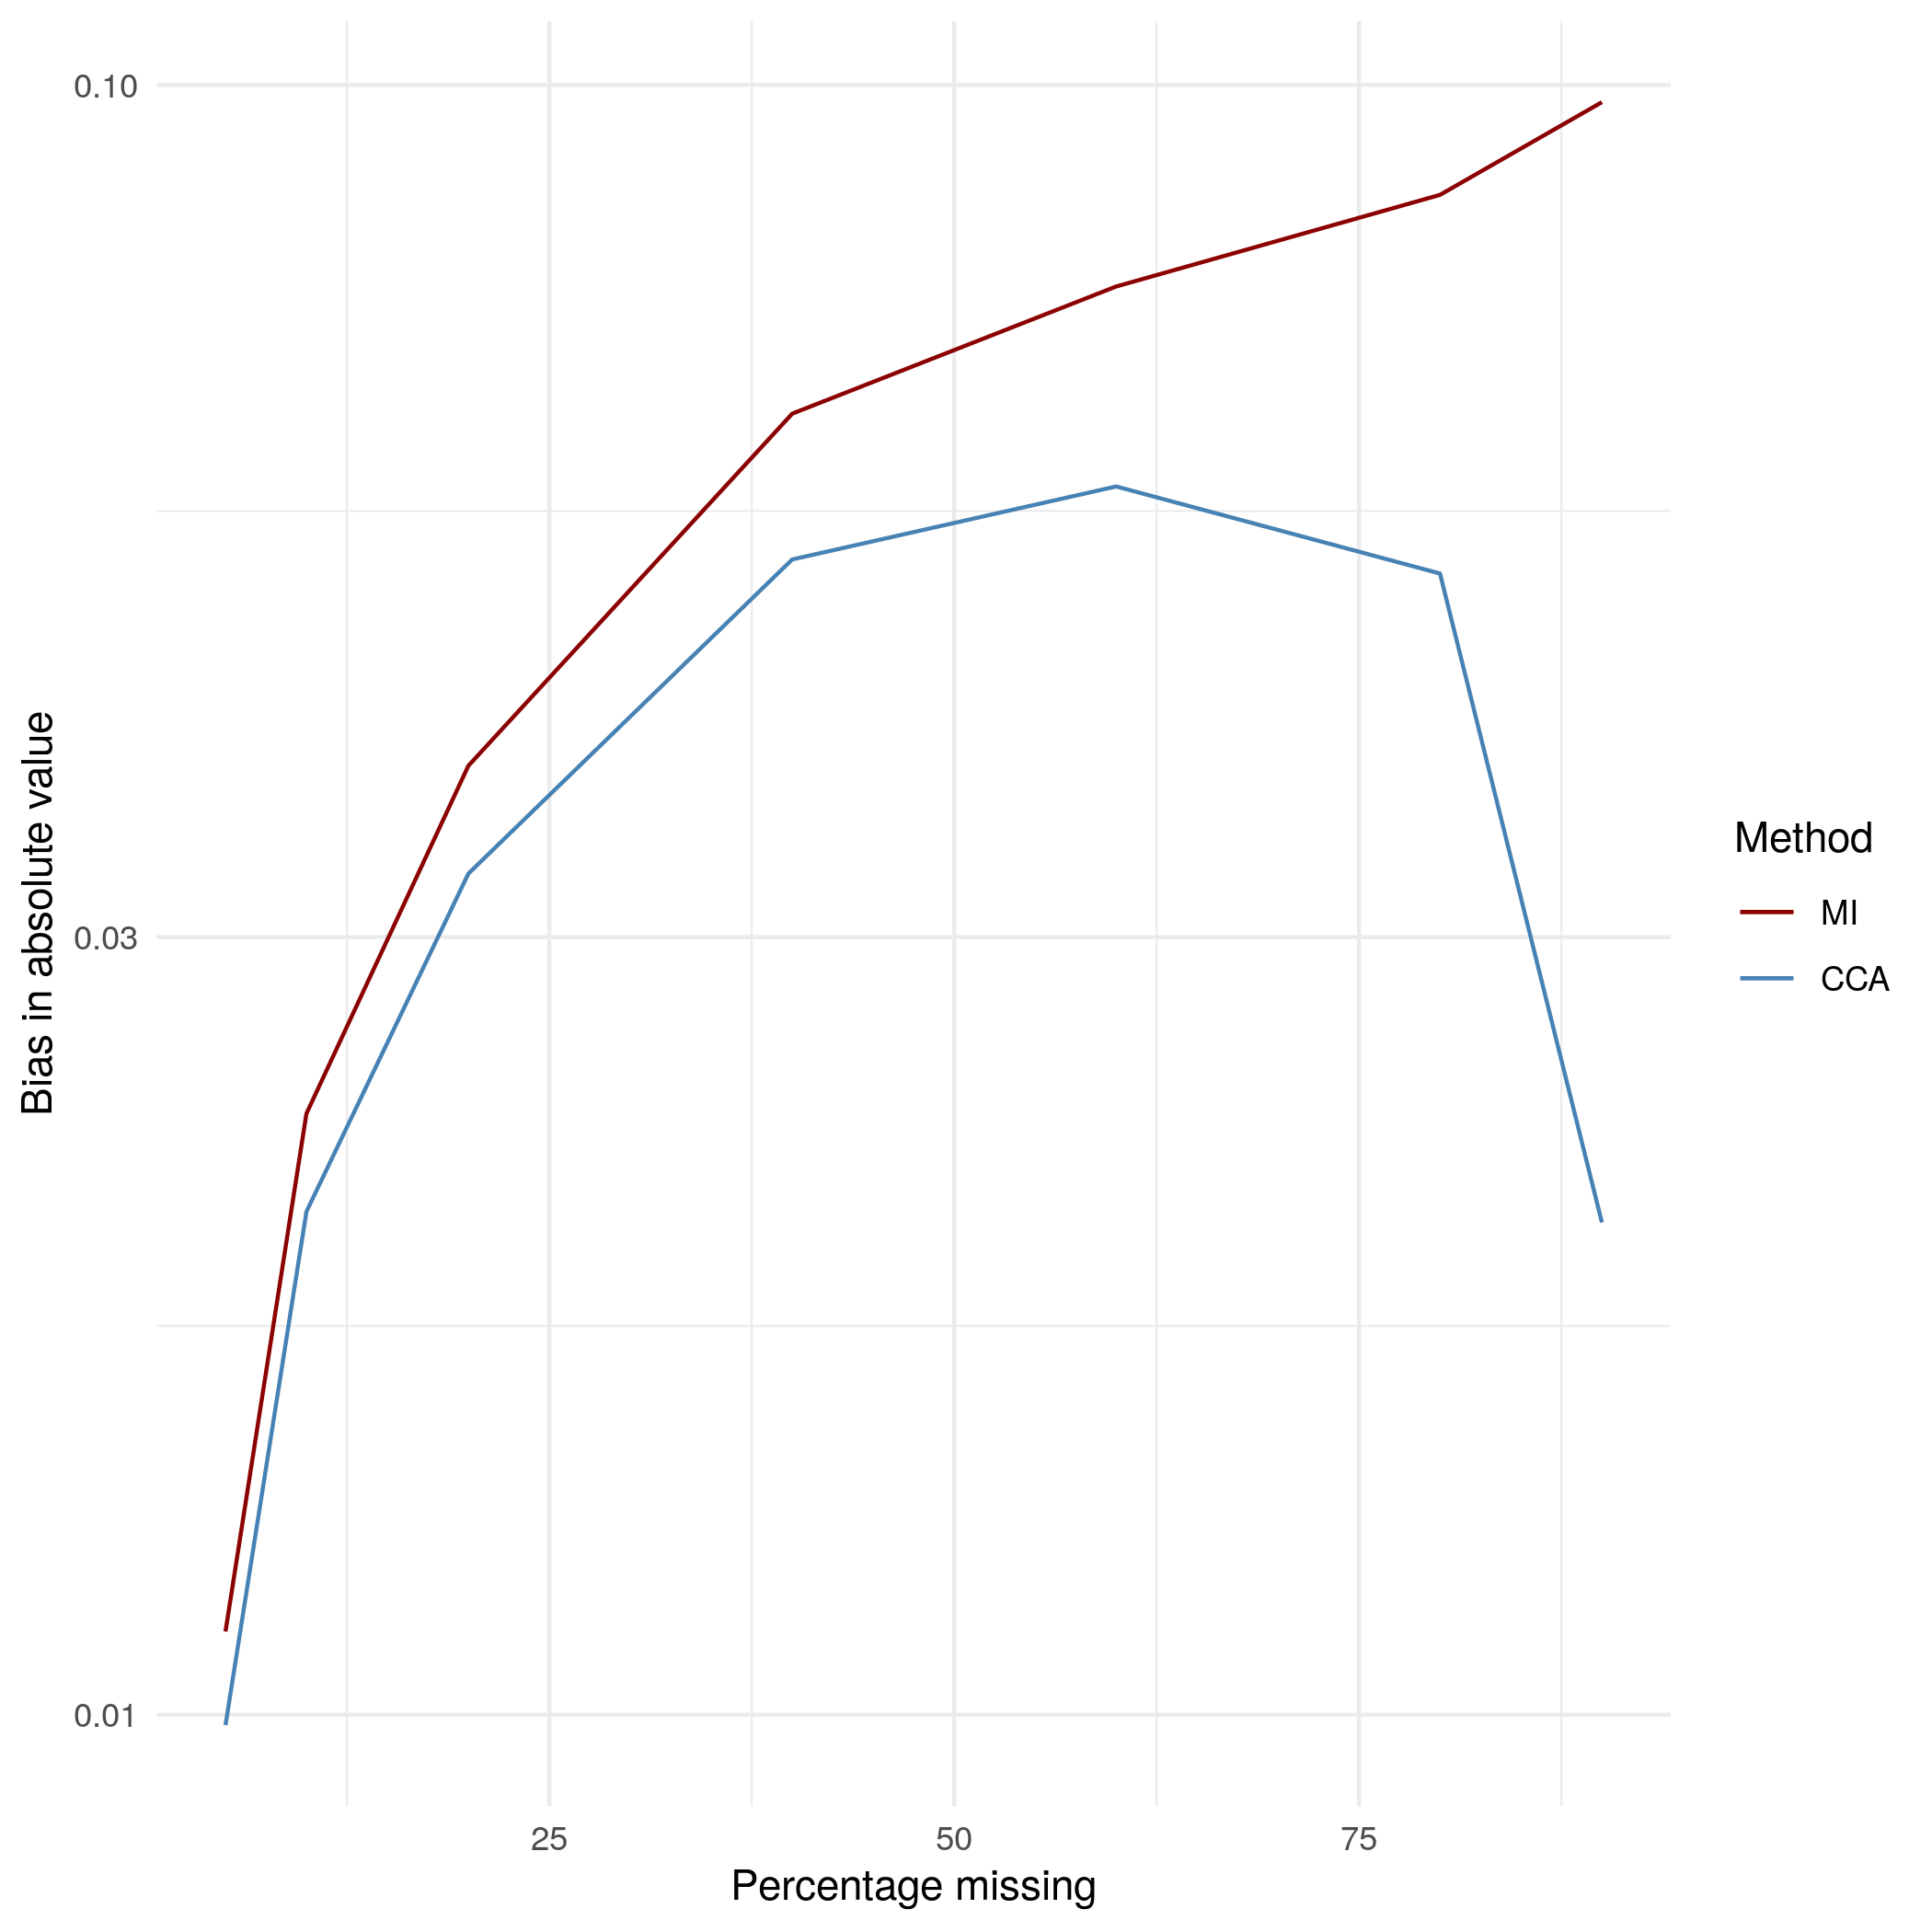
\includegraphics[width=0.3\textwidth]{mnar_final_bias.png}}
		\caption{Average results for MNAR missingness in $Y$ over 1000 repetitions of the analysis procedure described in 6.2.}
	\end{figure}
	We observe that both methods have a similar performance until they reach 60 percent missingness where their performance drastically diverges. Under MNAR, without specifying the missingness mechanism in the imputation model there is a high chance that it will be uncongenial with the analysis model. If this is the case, then this would go some way in explaining the poor performance of MI at hgih missingness.
	
	
	\subsection{Should we use multiple imputation?}
	Overall MI has shown quite poor performance in our experiments. Theory suggests that CCA should at best equal the performance of MI, and only in the MCAR scenario. We see from our experiments that multiple imputation loses some of its efficacy at extremely high levels of missingness. However, the research of Madley-Dowd et. al. [2019] suggest otherwise, showing that MI can yield large benefits for bias and standard error even at high missingness levels.  Madley-Dowd et. al. make use of auxiliary covariates, and so it is plausible that this has an impact on the performance of MI relative to our experiment. Given the vast amount of theory and experimental results on this topic, some of which has been cited in this thesis, the likely scenario is that the implementation has skewed the results.
	 
	
	\section{Conclusion and further work}
	This thesis has shown that missing data is an important consideration in data analysis by the effect it has on inference. The mechanism behind missing data is key to addressing it, and this thesis has characterised three possible such mechanisms. Imputation has been established as a statistically valid technique for addressing missing data. Various common and intuitive imputation methods such as Complete Case Analysis and Mean Imputation have been evaluated, with Multiple Imputation found to be the superior method. Theory and literature suggest strong benefits from using MI, however, this was not fully borne out in our own experiments. Nonetheless, the substantial amount of literature in favour of MI suggests that our experimental results were due to an error in implementation rather than an error with the method. Further study will be needed to verify this.
	
	Possible future investigations could be made into the effect of MI on prediction and classification, especially in the context of machine learning models. Another interesting avenue of exploration is replacing the conditional distributions with other modeling tools such as trees or neural networks. Perhaps the messy nature of much of modern data will make the underlying assumptions of conditional distributions untenable.

	\bibliography{final_5_bib}	
	\bibliographystyle{apalike}
	
\end{document}
